\documentclass[12pt]{report}
\usepackage[utf8]{inputenc}

\usepackage[a4paper,width=150mm,top=35mm,bottom=35mm,bindingoffset=6mm]{geometry}
\usepackage{caption}
\captionsetup[figure]{font=footnotesize}  %fontsize figute caption
%\usepackage{fancyhdr}
%\pagestyle{fancy}
\pagestyle{headings}
\usepackage{cite,mathtools,amsfonts}
\usepackage[dvipsnames]{xcolor}
\usepackage{ graphicx, calligra, amsmath, bm, multicol, braket,verbatim,amssymb,mathtools,standalone,hyperref,caption,subcaption,extarrows}
\usepackage{tikz,tikz-3dplot}
\usepackage{tikzscale}
\usetikzlibrary{decorations.markings}

\tikzstyle{axis} = [draw=black, line width=0.6mm , ->]
\tikzstyle{line} = [draw=black, line width=0.5mm]


\graphicspath{ {images/} }
\hypersetup{
    linktocpage,
    colorlinks=true,
    linkcolor=RoyalBlue, %blue!60!black,
    filecolor=magenta,      
    urlcolor=cyan,
    pdftitle={Lucas' Master project},
    pdfauthor={Lucas Freitas}
    pdfpagemode=FullScreen,
    citecolor=Purple,
}
\def \im{\dot{\imath}}
\def\bra#1{\mathinner{\langle{#1}|}}
\def\ket#1{\mathinner{|{#1}\rangle}}


\renewcommand{\bf}{\mathbf}
\renewcommand{\rm}{\mathrm}
\renewcommand{\cal}{\mathcal}

\usepackage{amsthm}
\usepackage[most]{tcolorbox}
\numberwithin{equation}{section}   
\newtheorem*{remark}{Remark}
\newtheorem*{theorem}{Theorem}
\newtheorem*{proposition}{Proposition}
\newtheorem*{corollary}{Corollary}
\renewcommand\qedsymbol{$\blacksquare$}

%\usepackage{biblatex}
%\addbibresource{references.bib}

\setlength{\parindent}{2em}
\setlength{\parskip}{1em}
%\setlength\columnsep{25pt}
\renewcommand{\baselinestretch}{1.2} % space btw lines

\usepackage{titlesec}    % for change the Chapter title fontsize
\titleformat{\chapter}[display]{\normalfont  \Large \bfseries}{\chaptertitlename\ \thechapter}{20pt}{ \LARGE }

\usepackage{dirtytalk}
\usepackage[xindy]{glossaries}
\renewcommand*{\glstextformat}[1]{\textcolor{black}{#1}} 
%normally the glossary link is related to the linkcolor of hyperlink; to adjust the color independently I need the above code. 
\makeglossaries

\newacronym{rucl}{$\alpha\text{-RuCl}_3$}{ruthenium trichloride}
\newacronym{hbz}{$\frac{1}{2}\text{BZ}$}{half Brillouin zone}
\newacronym{bz}{$\text{BZ}$}{Brillouin zone}
\newacronym{nn}{NN}{nearest-neighbor}
\newacronym{nnn}{NNN}{next-nearest-neighbor}
%\newacronym{nnn}{NNN}{Next Nearest Neighbor}
\newacronym{qsl}{QSL}{quantum spin liquid}
\newacronym{kqsl}{KSL}{Kitaev spin liquid}
\newacronym{nmr}{NMR}{nuclear magnetic resonance}
\newacronym{t1}{T1}{spin-lattice relaxation time}%{It is the time necessary to a material, under a constant magnetic field, to recovery to its equilibrium magnetisation value after a saturating pulse of the applied magnetic field.}
% Table of acronyms : I will try to use the minimal as possible  QSL , KQSL , NMR , 
% notation and definitions : T1 , \chi , \chi^{


% Cubic spin-lattice relaxation rate in Kitaev materials
\title{
{\large Universidade Federal do Rio Grande do Norte \\
Centro de Ciências Exatas e da Terra \\
Programa de Pós-Graduaç\~ao em Física \\ }
{\includegraphics[ width = 0.5 \textwidth]{ufrn_brasao_flat.pdf}} %\vspace{1cm}
{ \\ \textbf{Gapless excitations in Kitaev materials with defects}  } \\ %\vspace{1cm} 
{\small Natal - RN}
}
\author{\small Lucas Rodrigues Delgado de Freitas}
\date{ \small Fevereiro de 2021}



\begin{document}
\maketitle

\chapter*{Abstract}
%A \acrfull{qsl} appears in the notable Kitaev honeycomb spin-half model. The most promising Kitaev material, \acrshort{rucl}, is being tested for revealing gapless excitation. This work provide an explanation for this experimental measure as a result from the contribution from the Majorana modes localized in linear defects.

% explain the controversy: some experiments, such as the \acrfull(nmr), indicates the presence of gapless excitation in the \acrshort{kqsl};
% then explain: in this work I study the contribution of the Majoranas gapless modes to the relaxation rate in this gapped phase using the mean field approximation. 


A \acrlong{qsl} is a magnetic phase of matter that is remarkable for its ground state long-range entanglement and fractional excitations. A \acrlong{qsl}  appears in the well-known Kitaev honeycomb spin-half model. In a magnetic field, there is a phase transition to a topological phase with an energy gap in the bulk and chiral Majorana fermions at the edge. However, recent \acrlong{nmr} experiments suggest excitations without a gap in this phase, signalled by the cubic temperature dependence of the spin-lattice relaxation rate at low temperatures. 

In this work, I propose a mechanism to account for this experimental result. % based on the Kitaev model.
I use the localization of chiral Majorana modes in defects to explain the presence of gapless modes in the bulk. % The interaction between the chiral modes in the defects is treated with mean-field approximation.
Treating the weak interaction between the chiral modes in the defects within a mean-field approximation, I find that these modes remain gapless when the interaction is below a critical value that depends on the magnetic field strength. I used the effective low-energy theory to calculate the spin-lattice relaxation rate and found a behavior that agrees with the experimental result.

\textbf{Keywords}:
    Kitaev model, Quantum spin liquids, Majorana fermions, Mean-field, Nuclear relaxation rate.


% it has 192 words .

\chapter*{Resumo}

Um líquido quântico de spin é uma fase magnética da matéria que é  notável  pelo seu emaranhamento de longo alcance nos estados fundamentais  e excitações fracionalizadas.  Um líquido quântico de spin é realizado no modelo de Kitaev na rede hexagonal.  Sob aplicação de um campo magnético, tem-se uma transição de fase para uma fase topológica com um gap de energia no interior do material e férmions de Majorana quirais na borda. Entretanto, experimentos recentes de ressonância magnética nuclear indicam a existência de  excitações sem gap de energia nessa fase, indicada pela dependência cúbica na temperatura na taxa de relaxação spin-rede em baixas temperaturas.

Nesse trabalho, eu proponho um mecanismo para explicar esse resultado experimental. Eu utilizei a localização de modos de Majorana quiral em defeitos para explicar a presença de modos sem gap no interior do material. Tratando a interação entre os modos quirais nos defeitos por meio de aproximação de campo médio, eu encontrei que esses modos continuam sem gap quando a interação é mais fraca que um valor crítico dependente do campo magnético. Usei a teoria efetiva de baixas energias para calcular a taxa de relaxação spin-rede e encontrei um valor que concorda com o resultado experimental.

\textbf{Palavras-chave}:
    Modelo de Kitaev,
    Líquidos quânticos de spin,
    Férmions de Majorana,
    Campo médio,    
    Taxa de relaxação nuclear.

%\chapter*{Dedication} To ...
% \chapter*{Declaration} I declare that..
%\chapter*{Acknowledgements}
%I want to thank...


\renewcommand{\baselinestretch}{.01} 
\setlength{\parindent}{.01em}
\tableofcontents
\listoffigures 


\clearpage
\printglossary
\setlength{\parindent}{2em}
\renewcommand{\baselinestretch}{1.35} 


\chapter{Introduction}






The interplay of topology and strongly correlated phenomena gives rise to fascinating physics such as the fractionalization of elementary particles.  An important example is the fractional quantum Hall effect, in which the electronic degrees of freedom split into quasiparticles with fractional electron charge. Another prominent example is the central theme of this work: the \acrfull{qsl} \cite{Balents2010, Savary_2016, Knolle_2019, Misguich2011}. In magnetic insulators, these phases of matter exhibit long-range coherence, but fluctuation prevents the formation of magnetic order even at zero temperature.

A remarkable example of \acrshort{qsl} is the \acrfull{kqsl} proposed as a toy model by A. Kitaev in 2006 \cite{Kitaev_2006}. This strongly interacting spin system has as its elementary excitation $\mathbb{Z}_2$-vortices and Majorana fermions. Upon applying a magnetic field, the Majoranas become gapped with a Chern insulator spectrum. The non-trivial topology of this insulator gives rise to chiral Majorana modes at the edge. Unlike the fractional quantum Hall effect, the edge modes with opposite chiralities in \acrshort{kqsl} are electrically neutral. %occur in two fermionic species of opposite chiralities and are electrically neutral. %and Chern number  $\pm 1$. 

In previous work, \cite{Kitaev_2003}, Kitaev had proposed that non-Abelian anyons could be used to realize a physical error-correction quantum code. The anyonic system provides a realization of a quantum memory that is protected from decoherence. This remarkable property raised attention for theoretical models with this type of particle since the current major limitation to construct a useful quantum computer is the frequent errors caused by decoherence. The quantum computers (theoretically) made using these models are named topological quantum computers \cite{Nayak2008, Stern1179}.  The Kitaev model was constructed with the purpose of creating a two-dimensional spin model whose elementary were non-Abelian anyons.

The Kitaev model was not created with a physical realization in mind. Nevertheless, a few years later Jackeli and Khaliullin \cite{Jackeli_2009} proposed a mechanism for a Mott insulator with dominant Kitaev interaction. The first studied materials were the iridates, $\text{A}_2\text{IrO}_3$ (A = Na,Li), which realize the Kitaev model plus additional small non-Kitaev interaction. The model that include those non-Kitaev interactions is called \textit{extended Kitaev model} or $J\text{-}K\text{-}\Gamma$, $J$ for the Heisenberg interaction, $K$ for the Kitaev interaction, and $\Gamma$ for the off-diagonal interactions.  % isotropic exchange (J) and anisotropic  The material \acrshort{rucl} became more popular as was discovered that 

Even though the non-Kitaev interactions are small in the iridate materials, they are sufficient to drive a zigzag order for weak magnetic fields \cite{Choi-2012,Ye-2012}. Therefore, the iridates do not  have a \acrshort{qsl} ground state. Furthermore, for strong fields, the material goes through a phase transition to a paramagnetic phase, a trivial partially polarized state. %(forced ferromagnetic order). 
There is a small window of magnetic fields in which a \acrshort{qsl} may exist. %A similar, but slightly better, situation happens for \acrfull{rucl}. The similar limitation happens in the magnetic field domain, however the Néel temperature ($T_N$) is much smaller for this ruthenium material than for iridate ones. % This behaviour is probably due d
A similar situation happens for \acrfull{rucl}. However, it is slightly better since the Néel temperature ($T_N$) is much smaller for this ruthenium material than for iridate ones.

%%%%%%%%%%%%%%%%%%%%%%%%%%%%%%%%%%
%%%%%%%%%%%%%%%% Rewrite this paragraph
One experimental group tested the spin-orbit Mott insulator \acrshort{rucl} and found evidence for a thermal quantum Hall effect \cite{Kasahara_2018,yokoi2020halfinteger}. % Unlike the Integer or Fractional Hall Effects, the Kitaev Spin Liquid excitation are neutral. 
While the elementary excitation of \acrshort{kqsl} are neutral, they can carry energy and therefore contribute to  heat transport. The experiment was done using a temperature gradient %introduce a current of phonons in the edge to interact thermally with the Majorana. 
The theory for \acrshort{kqsl} predicts that the \acrshort{rucl} exhibits a  quantization of the transverse thermal conductivity $\kappa_{xy}$. The experimental results are not sharp and clear, but the authors of \cite{Kasahara_2018} believe they found the thermal Hall effect in a region of moderate magnetic fields 7--9T.
% see the articles  \cite{Ye_2018,Aviv_2018}
The value measured for $\kappa_{xy}$ is not equal to the ideal conductivity of an isolated edge mode. There are proposals to explain this difference because of the coupling between the phonons and the Majorana edge modes \cite{Ye_2018,Aviv_2018}.



%\textcolor{red!40!black}{One candidate material for the \acrfull{kqsl} is \acrshort{rucl}. It is believed to behave as a \textbf{gapped} \acrshort{qsl} in a region of intermediate field $(8\sim10\text{ Tesla}$). In this introduction I want to give a short review about the recent experiments that rises the doubts about the \acrshort{rucl} to be a gapped or a gapless phase inthis region.\begin{itemize}    \item Introduction to Kitaev material (which \textbf{articles ?}   );    \begin{itemize}        \item Articles about \acrlong{qsl} : ;        \item Quantum computation (application) : \cite{Nayak2008};        \item About the theory of the \acrlong{kqsl}: \cite{Kitaev_2006, Jackeli_2009}    \end{itemize}    \item Review of experiments about the gap in  \acrshort{rucl} ( e.g. \cite{Zheng-gapless2017, Baek2017, Nagai_2020, tanaka2020} );    \item Interaction between chiral Majorana edges modes : \cite{Aasen_2020} .\end{itemize}}

%A fractional excitation is non-local in the spin operator. In fact, for a spin-half system the ladder operator for spin $S_{i}^{+}$ and $S_{i}^{-}$ can change the total magnetisation $S^{z}_{\text{total}}$ in integer values (units of $\hbar = 1$).


A recent \acrfull{nmr} experiment found unexpected results \cite{Zheng-gapless2017}. From the theory of Kitaev materials,  \acrshort{rucl} should behave as a gapped \acrshort{qsl} under not too strong magnetic fields. This behavior was experimentally verified in  thermal Hall measurements in \cite{Kasahara_2018,yokoi2020halfinteger} and specific heat measurements \cite{tanaka2020}. However,  this \acrshort{nmr} experiment found a spin-lattice relaxation rate of $T_1^{-1} \propto T^3$, which is rather expected for a gapless fermionic system. In the words of the authors of \cite{Zheng-gapless2017}: \say{\textit{our NMR results show unequivocally that the spin excitations themselves are gapless, and thus such proximate Kitaev physics appears to be excluded. [...] This result cannot be reconciled with the behavior of conventional quantum magnets or of the pure or generic Kitaev QSL}}.  

Another \acrshort{nmr} experiment \cite{ Baek2017} claimed to observe a behavior $T_1^{-1} \propto e^{-\Delta/T}$, but only in the regime of large magnetic fields where the gap must be associated with magnons in the trivial paramagnetic phase. In \cite{Nagai_2020}, the temperature dependence of $1/T_1$ was fitted to a double exponential in an attempt to extract two different energy scales associated with Majorana fermions and vortices.
%On the other hand, was experimentally found others $T_1$ behaviours, e.g. $T_1^{-1} \propto e^{-\Delta/T}$ \cite{ Baek2017} or more complicated \cite{Nagai_2020}, that agree with the gapped nature of the excitation in \acrshort{rucl}.
A very recent thermal transport experiment,\cite{Hentrich_2020}, founded evidence for defect-induced low-energy excitations in the longitudinal heat conductivity for \acrshort{rucl}.

On theoretical grounds, Kitaev materials under moderate magnetic fields should exhibit gapless Majorana fermions at the edge, but the \acrshort{nmr} experiments on an ideal material would probe the bulk excitation which is gapped. In this work, I explore the possibility that the observed gapless mode in the bulk is due to Majorana fermions localized along with linear defects in the material. % A reasonable explanation to found gapless excitation in the bulk is due to the presence of localised Majorana fermions in linear defects of the material. 
It is known that stacking faults in layered materials may induce the formation of linear defects such as partial dislocations \cite{solyom-solids}.
Indeed, \acrshort{rucl} is a quasi-two-dimensional material with weakly interacting layers that can easily slip on one another producing stacking faults \cite{Kim_Kee_2016,Cao_2016,Ran2017,Zheng-SM2017}.

This work is a study of linear defects in the pure Kitaev model. As a first theoretical model, I focus on a particular type of linear defects in which the structure resembles a zigzag edge. The toy model for this defect consists of seaming two semi-infinite \acrshort{kqsl}. At my starting point, both subsystems contain chiral edge modes, which I then couple by an exchange interaction that is weaker along with the defect than in the bulk. My model is inspired by Ref.\cite{Aasen_2020}, which noted that there is a critical value of the exchange interaction between edges below which the chiral modes remain decoupled. From the point of view of the  low-energy  effective theory, the reason is that the weak interaction between emergent Majorana fermions is irrelevant in the renormalization group sense. %The interaction between the edges is irrelevant, and for weak interaction the model is a effective a free Majorana system. Some of the idea of proximate two Kitaev materials was inspired by \cite{Aasen_2020}, which uses this mechanism for a different purpose.

In contrast to the field theoretical arguments of Ref.\cite{Aasen_2020}, here I first study the critical condition for seaming the one-dimensional Majorana modes directly in the lattice model. First, I calculate the spectrum using a self-consistent mean-field approximation for the exchange interaction along with the defect. Having identified the regime of decoupled gapless modes, I proceed by explicitly deriving the representation of the spin operator in the low-energy sector as a Majorana fermion bilinear. Following, I then use the effective field theory to compute the dynamical spin-spin correlation function which determines the spin-lattice relaxation rate at low temperatures. I find the power-law dependence $T_1^{-1} \propto T^3$, in agreement with the experimental results of Ref.  \cite{Zheng-gapless2017}.

This dissertation is organized as follows. In chapter \ref{ch:2}, I will set the notation and review the important aspects of the Kitaev model. Complementary, the description of the model in a more convenient geometry with zigzag edges is presented in chapter \ref{ch:3}. The defects are described %The description of the defects is made
in chapter \ref{ch:4} in which mean-field approximation  is used to deal with the interaction across the \say{edges} of the defect. The approximation gives ground to describe the low-energetic excitation localized in the defect as Majorana fermions, the passage from the microscopic theory to this effective theory is described in chapter \ref{ch:5}. The spin-lattice relaxation rate, $1/T_1$, is calculated in chapter \ref{ch:6}.

















\chapter{The Kitaev honeycomb model}
\label{ch:2}
The Kitaev and related models attracted much interest in both theoretical and experimental communities in the last decade. Remarkably, they exhibit an exact \acrshort{qsl} ground state and potentially can be experimentally realized in Mott insulating magnets with strong spin-orbit coupling \cite{Jackeli_2009, trebst2017kitaev, takagi2019}. These reasons show how peculiar and fascinating the Kitaev model is.

Another remarkable property of the model is its elementary excitations. The low energy spin excitations about the ground state fractionalize into Majorana fermions and $\mathbb{Z}_2$-vortices. Depending on the anisotropy of the interaction between the spins, at zero magnetic fields, the ground state can happen in two classes of phases. There are three similar but algebraically distinct gapped phases: $A^x,A^y,A^z$. This phase includes the strong anisotropic limit in which the Majoranas and the vortices have Abelian anyonic statistics. On the flip side, there is a fourth phase, named $B$, in which the Majoranas are gapless. This work will to most of its extent be center on the isotropic limit, which happens inside this phase.

Importantly, the $B$ phase becomes gapped in the presence of a magnetic field, which gives topological non-trivial properties such as non-Abelian anyonic statistics and non-zero Chern number for the Majorana fermions living in this phase.

This chapter has the fundamental purpose of introducing the reader to the well-known theory \cite{Kitaev_2006} of the Kitaev honeycomb model assuming a system with periodic boundary conditions. 

\begin{comment}
\textcolor{red!40!black}{
 The chapter will be divided as follow:
\begin{itemize}
    \item shortly describing the model without magnetic field   (basically chapters $1$,$2$ and $4$ of the article ): describe the lattice, the Hamiltonian, the transformation to Majorana, bond variable, flux sectors, a solution with Fourier transform, the phase diagram and the \textbf{dispersion}; 
    \item with magnetic field in perturbation theory (chapter $6$ of the article );
    \item about the elementary excitation (chapters $7$ and $8$).
\end{itemize}
The purpose of the chapter is to tell the relevant aspects of the model. I will not prove anything.
}
(HERE DESCRIBE THE LATTICE: HONEYCOMB, EVEN-ODD, PICTURE)
\end{comment}




\section{The model}


The Kitaev model consists of spins-1/2 in a lattice of coordination three with Ising-like interactions between \acrfull{nn} spin depending upon the bond type. In addition, I can consider the effects of time-reversal symmetry breaking term due to a magnetic field. In this work, I will work with the two-dimensional Kitaev model, which has a honeycomb type lattice. 

The honeycomb lattice is bipartite. This means that it can be subdivided in two triangular sub-lattices which are denoted by \say{even} sublattice $\mathcal{L}_{\text{E}} $ (white circle) and the  \say{odd} $ \mathcal{L}_{\text{O}}$ (black circles) which are shown in figure \ref{fig:lattice_zigzag}. 




%The literature do not have a consensus in the notation for the Kitaev operator and the letter for the interaction.
There is no consensus in the literature regarding the notation for the Kitaev model. I will follow Kitaev's notation and use $J^{\gamma}$ for the interaction and write the spin operators in terms of the Pauli operators
\begin{equation}
    S^{\gamma}_j \; = \; \frac{1}{2} \sigma^{\gamma}_{j} \;, \quad  \text{for } \gamma = x,y,z.
\end{equation}
Where the spin operators obey the $\textrm{SU}(2)$ algebra, e.g.
\begin{equation}
    [ \, S^{x}_j , S^{y}_k \, ] \; = \; \im \delta_{jk}  \, S^{z}_j \; .
\end{equation}
\begin{figure}[h]
    \centering
    \scalebox{1.5}{\documentclass{standalone}  
\usepackage{tikz,comment}
\usepackage[active,tightpage]{preview}
\PreviewEnvironment{tikzpicture}
\setlength\PreviewBorder{1pt}
%%%
\usetikzlibrary{arrows} 





\begin{document}
% Define the layers to draw the diagram
\pgfdeclarelayer{background}
\pgfdeclarelayer{foreground}
\pgfsetlayers{background,main,foreground}


\def \h { 0.57735026918}  % 1/sqrt(3) comprimento  y  de uma celula                                     even (White, 2y) to odd (black ,2y+1) 
\def \d { 0.28867513459}  % 1/ 2 sqrt(3)  distancia  y  entre celulas                                   odd (black , 2y-1) to even (white , 2y)
\def \c { 0.5}           % 1/2 distancia  x  entre celulas  
\def \v { 0.86602540378 }  % sqrt(3)/ 2   distancia  y  de duas celulas                                   odd-odd or even-even 


\def \mar {0.2}  % margin for the clip

\def \l {7}         %horizontal length

\begin{tikzpicture}[>=latex]






\clip (-\mar+1,  \v -2*\d -2*\d-2*\v -\mar ) rectangle (\l+\mar+1,\v+\mar);


\foreach \a in {0,...,\l}{
        \draw[draw=blue!80!black, line width=0.40mm] ( \c +\a, \v  )-- ( \c+\a, \v + \c);
        \draw[draw=blue!80!black, line width=0.40mm] ( \c+\a, -\d )-- ( \c+\a, -\d -\v+\d);
        \draw[draw=blue!80!black, line width=0.40mm] ( \c +\a, \v -\c-2*\d-2*\v )-- ( \c+\a, \v -\c -\c-2*\d-2*\v);
}

\node at ( \c+4-.05, -\d - .25) [right] { \scriptsize \textcolor{blue!75!black}{$J_z$}   };
\node at ( \c+4.2, -\v-.12) [below] { \scriptsize \textcolor{green!75!black}{$J_y$}   };
\node at ( \c+4-.065
, -\d - .55) [left] { \scriptsize \textcolor{red!75!black}{$J_x$}   };

\foreach \b in {-1,0}{    
    \foreach \a in {1,3,...,\l} {
        \draw[draw=green!80!black, line width=0.40mm] ( \a , -\d +\v+ 2*\v*\b    ) -- ( \a -\c, -\d +\v+ 2*\v*\b   +\d );
        \draw[draw=red!80!black, line width=0.40mm] (\a , -\d +\v+ 2*\v*\b - \v+\d )-- ( \a -\c,  -\d +\v+ 2*\v*\b - \v);
            }   
}


\foreach \b in {-1,0}{    
    \foreach \a in {1,3,...,\l} {        
        \node[circle, fill=white, draw=black, line width=0.40mm, inner sep=2pt, minimum size=2pt] (W1\b\a) at ( \a , -\d +\v+ 2*\v*\b    ) {};
    	\node[circle, fill=black, draw=black, line width=0.40mm, inner sep=2pt, minimum size=2pt] (B2\b\a) at ( \a + \c, \v + 2*\v*\b   ) {};
        \node[circle, fill=white, draw=black, line width=0.40mm, inner sep=2pt, minimum size=2pt] (W3\b\a) at ( \a +1, -\d +\v+ 2*\v*\b    ) {};
    	\node[circle, fill=black, draw=black, line width=0.40mm, inner sep=2pt, minimum size=2pt] (B4\b\a) at ( \a +1, -\d +\v+ 2*\v*\b - \v+\d)  {};
    	\node[circle, fill=white, draw=black, line width=0.40mm, inner sep=2pt, minimum size=2pt] (W5\b\a) at ( \a -\c + 1, -\d +\v+ 2*\v*\b - \v) {};  	
    	\node[circle, fill=black, draw=black, line width=0.40mm, inner sep=2pt, minimum size=2pt] (B6\b\a) at  ( \a , -\d +\v+ 2*\v*\b - \v+\d ) {};

    	\node[circle, fill=black, draw=black, line width=0.40mm, inner sep=2pt, minimum size=2pt] (B2r\b\a) at ( \a + \c+1, -\d +\v+ 2*\v*\b+\d   ) {}; 
    	\node[circle, fill=white, draw=black, line width=0.40mm, inner sep=2pt, minimum size=2pt] (W5r\b\a) at ( \a -\c + 2, -\d +\v+ 2*\v*\b - \v) {};    	
    	
    }   
}

\foreach \b in {-1,0}{    
    \foreach \a in {1,3,...,\l} { 
        \draw[draw=red!80!black, line width=0.40mm] (B2\b\a)-- (W1\b\a);
        \draw[draw=green!80!black, line width=0.40mm] (B2\b\a)--(W3\b\a);
        \draw[draw=blue!80!black, line width=0.40mm] (W1\b\a)--(B6\b\a);
 %       \draw[draw=green!80!black, line width=0.40mm] (W1\b\a)-- ( \a -\c, -\d +\v+ 2*\v*\b   +\d );
        \draw[draw=red!80!black, line width=0.40mm] (B2r\b\a)-- (W3\b\a);        
        \draw[draw=blue!80!black, line width=0.40mm] (W3\b\a)--(B4\b\a);       
        \draw[draw=green!80!black, line width=0.40mm] (W5\b\a)--(B6\b\a);        
        \draw[draw=red!80!black, line width=0.40mm] (B4\b\a)-- (W5\b\a);
        \draw[draw=green!80!black, line width=0.40mm] (W5r\b\a)--(B4\b\a); 
%        \draw[draw=red!80!black, line width=0.40mm] (B6\b\a)-- ( \a -\c, 2*\v*\b   - \d);
            }   
}


\draw[->,draw=cyan!80!black, line width=0.3mm] (0.01+3,-\d-\v - 0.01 + \v + \d)--( -1+\c - 0.08+3, -\d +0.125 + \v +\d ) node[below = 6pt] { \textcolor{cyan!80!black}{$n_{2}\, $} };
\draw[->,draw=cyan!80!black, line width=0.3mm] ( -0.01+3,-\d -\v - 0.01 + \v + \d)--(\c + 0.08+3, -\d + 0.125 + \d+ \v ) node[below = 6pt] {\textcolor{cyan!80!black}{$\, n_{1}$}};

\draw[->,draw=orange!70!gray, line width=0.3mm] (-2+8,0)--( -2+\c+0.085+8, -\d-0.05 ) node[midway,below] { \textcolor{orange!70!gray}{$e_{2} \, $} };
\draw[->,draw=orange!70!gray, line width=0.3mm] (-2+8,0)--( -3+\c -0.085+8, -\d- 0.05 ) node[midway,below] { \textcolor{orange!70!gray}{$\,e_{3}$} };
\draw[->,draw=orange!70!gray, line width=0.3mm] (-2+8,0)--( -2+8, -\d+\v+0.11 ) node[midway,right] { \textcolor{orange!70!gray}{$e_{1}$} };

\end{tikzpicture}
\end{document}}
    \caption{Honeycomb lattice with unit cell along the vertical direction. The unit vectors $n_1=(\frac{1}{2},\frac{\sqrt{3}}{2})$ and $n_2=(-\frac{1}{2},\frac{\sqrt{3}}{2})$ are the basis vector that span a triangular Bravais lattice, and $e_1$, $e_2$ and $e_3$ are the \acrshort{nn} vectors (with length $1/\sqrt{3}$). Colors red, green and blue along the bonds represent a Ising-like interactions $J_x \sigma^{x}_{j}\sigma^{x}_{j+e_3}$, $J_y\sigma^{y}_{j}\sigma^{y}_{j+e_2}$ and $J_z \sigma^{z}_{j}\sigma^{z}_{j+e_1}$ respectively.
    }
    \label{fig:lattice_zigzag}
\end{figure}


The Kitaev model is described by a sum of local bilinears in the spin, which depend upon the direction of the bond. The Hamiltonian is
\begin{equation}
    H \; = \; -   \, \sum_{\, \langle i,j \rangle_{\gamma} }  \, J_{\gamma} \sigma_{i}^{\gamma} \sigma_{j}^{\gamma} \; , %    \; - \; \kappa  \sum_{ \,  \langle i,j,k \rangle_{\gamma} }   \sigma_{i}^{x} \sigma_{j}^{y} \sigma_{k}^{z} \; ,
\end{equation}
where $ \sigma_{i}^{\gamma}$ is the Pauli operator in the $\gamma \in \{ x , y , z \} $ direction at the position $i$ on the honeycomb lattice. The sum on the first term runs over \acrshort{nn} sites. %The second term is the contribution of the magnetic field in third order in the perturbation theory and the sum is over .



\begin{figure}[t]
    \centering
    \begin{subfigure}{.45\textwidth}
        \centering
        \scalebox{1.5}{\input{Tikz/CH2/T:2-plaq-notation} } 
        \caption{Notation for the sites in a plaquette.}
        \label{fig:2-plaquette-notation}
    \end{subfigure} \hspace{5mm}%
    \begin{subfigure}{.45\textwidth}
        \centering
        \scalebox{1.5}{\documentclass{standalone}  
\usepackage{tikz,comment}
\usepackage[active,tightpage]{preview}
\PreviewEnvironment{tikzpicture}
\setlength\PreviewBorder{1pt}
%%%
\usetikzlibrary{arrows} 





\begin{document}
% Define the layers to draw the diagram
\pgfdeclarelayer{background}
\pgfdeclarelayer{foreground}
\pgfsetlayers{background,main,foreground}


\def \h { 0.57735026918}  % 1/sqrt(3) comprimento  y  de uma celula                                     even (White, 2y) to odd (black ,2y+1) 
\def \d { 0.28867513459}  % 1/ 2 sqrt(3)  distancia  y  entre celulas                                   odd (black , 2y-1) to even (white , 2y)
\def \c { 0.5}           % 1/2 distancia  x  entre celulas  
\def \v { 0.86602540378 }  % sqrt(3)/ 2   distancia  y  de duas celulas                                   odd-odd or even-even 


\def \mar {0.44}  % margin for the clip

\def \l {7}         %horizontal length

\begin{tikzpicture}[>=latex]






\clip (-\mar+1,  \v -\d-\v -\mar ) rectangle (1+\mar+1+.05,\v+\mar);


\foreach \a in {0,1}{
        \draw[draw=blue!80!black, line width=0.40mm] ( \c +\a, \v  )-- ( \c+\a, \v + \c);
        \draw[draw=blue!80!black, line width=0.40mm] ( \c+\a, -\d )-- ( \c+\a, -\d -\v+\d);
        \draw[draw=blue!80!black, line width=0.40mm] ( \c +\a, \v -\c-2*\d-2*\v )-- ( \c+\a, \v -\c -\c-2*\d-2*\v);
}

\node at ( \c+4-.05, -\d - .25) [right] { \scriptsize \textcolor{blue!75!black}{$J_z$}   };
\node at ( \c+4.2, -\v-.12) [below] { \scriptsize \textcolor{green!75!black}{$J_y$}   };
\node at ( \c+4-.065
, -\d - .55) [left] { \scriptsize \textcolor{red!75!black}{$J_x$}   };

\foreach \b in {-1,0}{    
    \foreach \a in {1,3} {
        \draw[draw=green!80!black, line width=0.40mm] ( \a , -\d +\v+ 2*\v*\b    ) -- ( \a + \c-1, \v + 2*\v*\b   );
        \draw[draw=red!80!black, line width=0.40mm] (\a , -\d +\v+ 2*\v*\b - \v+\d )-- ( \a -\c, -\d +\v+ 2*\v*\b - \v);
            }   
}


\foreach \b in {-1,0}{    
    \foreach \a in {1,3} {        
        \node[circle, fill=white, draw=black, line width=0.40mm, inner sep=2pt, minimum size=2pt] (W1\b\a) at ( \a , -\d +\v+ 2*\v*\b    ) {};
    	\node[circle, fill=black, draw=black, line width=0.40mm, inner sep=2pt, minimum size=2pt] (B2\b\a) at ( \a + \c, \v + 2*\v*\b   ) {};
        \node[circle, fill=white, draw=black, line width=0.40mm, inner sep=2pt, minimum size=2pt] (W3\b\a) at ( \a +1, -\d +\v+ 2*\v*\b    ) {};
    	\node[circle, fill=black, draw=black, line width=0.40mm, inner sep=2pt, minimum size=2pt] (B4\b\a) at ( \a +1, -\d +\v+ 2*\v*\b - \v+\d)  {};
    	\node[circle, fill=white, draw=black, line width=0.40mm, inner sep=2pt, minimum size=2pt] (W5\b\a) at ( \a -\c + 1, -\d +\v+ 2*\v*\b - \v) {};  	
    	\node[circle, fill=black, draw=black, line width=0.40mm, inner sep=2pt, minimum size=2pt] (B6\b\a) at  ( \a , -\d +\v+ 2*\v*\b - \v+\d ) {};

    	\node (B2r\b\a) at ( \a + \c+1, -\d +\v+ 2*\v*\b+\d   ) {}; 
    	\node (W5r\b\a) at ( \a -\c + 2, -\d +\v+ 2*\v*\b - \v) {};    	
    	
    }   
}

\foreach \b in {-1,0}{    
    \foreach \a in {1,3} { 
        \draw[draw=red!80!black, line width=0.40mm] (B2\b\a)-- (W1\b\a);
        \draw[draw=green!80!black, line width=0.40mm] (B2\b\a)--(W3\b\a);
        \draw[draw=blue!80!black, line width=0.40mm] (W1\b\a)--(B6\b\a);
 %       \draw[draw=green!80!black, line width=0.40mm] (W1\b\a)-- ( \a -\c, -\d +\v+ 2*\v*\b   +\d );
        \draw[draw=red!80!black, line width=0.40mm] (B2r\b\a)-- (W3\b\a);        
        \draw[draw=blue!80!black, line width=0.40mm] (W3\b\a)--(B4\b\a);       
        \draw[draw=green!80!black, line width=0.40mm] (W5\b\a)--(B6\b\a);        
        \draw[draw=red!80!black, line width=0.40mm] (B4\b\a)-- (W5\b\a);
        \draw[draw=green!80!black, line width=0.40mm] (W5r\b\a)--(B4\b\a); 
%        \draw[draw=red!80!black, line width=0.40mm] (B6\b\a)-- ( \a -\c, 2*\v*\b   - \d);
            }   
}

\node (p) at (1.5,\v*.5-\d*.5) { \small $W_p$ };
\foreach \b in {0}{    
    \foreach \a in {1} { 
\node[below=3pt] (p1) at ( \a , -\d +\v+ 2*\v*\b - \v+\d ) { \tiny \textcolor{red!80!black}{$\sigma_{p_1}^{x}$} };
\node[below left =.01pt] (p2) at ( \a+.1 , -\d +\v+ 2*\v*\b    ) { \tiny \textcolor{green!80!black}{$\sigma_{p_2}^{y}$} };
\node[left =2pt] (p3) at ( \a + \c, \v + 2*\v*\b +.1  ) { \tiny \textcolor{blue!80!black}{$\sigma_{p_3}^{z}$} };
\node[above=3pt] (p4) at ( \a +1, -\d +\v+ 2*\v*\b    ) { \tiny \textcolor{red!80!black}{$\sigma_{p_4}^{x}$} };
\node[above right =.01pt] (p5) at ( \a +1-.04, -\d +\v+ 2*\v*\b - \v+\d) { \tiny \textcolor{green!80!black}{$\sigma_{p_5}^{y}$} };
\node[below right = 0.1pt] (p6) at ( \a -\c + 1, -\d +\v+ 2*\v*\b - \v + .1) { \tiny \textcolor{blue!80!black}{$\sigma_{p_6}^{z}$} };
} }

%          \sigma_{p_1}^{x}\sigma_{p_2}^{y}\sigma_{p_3}^{z}\sigma_{p_4}^{x}\sigma_{p_5}^{y}\sigma_{p_6}^{z}


\end{tikzpicture}
\end{document} }
        \caption{Wilson operator and the spins point outwards.% Similar to magnetic flux.
        }
        \label{fig:2-plaquette-spin}
    \end{subfigure}
\caption{Each plaquette $p$ in the honeycomb lattice contain six sites $j=p_1,...,p_6$. The notation used follows Kitaev. Note that black circles have even subindex and white circle have odd subindex in agreement to the sublattice names. A Wilson loop operator $W_p$ is defined for each plaquette $p$ by the equation.}
\end{figure}
%\begin{figure}[h!]  \begin{minipage}{.2\textwidth}    \centering    \scalebox{1.5}{\input{Tikz/CH2/T:2-plaq-notation} }   \end{minipage}%  \begin{minipage}{.8\textwidth}    \centering    \scalebox{1.5}{\documentclass{standalone}  
\usepackage{tikz,comment}
\usepackage[active,tightpage]{preview}
\PreviewEnvironment{tikzpicture}
\setlength\PreviewBorder{1pt}
%%%
\usetikzlibrary{arrows} 





\begin{document}
% Define the layers to draw the diagram
\pgfdeclarelayer{background}
\pgfdeclarelayer{foreground}
\pgfsetlayers{background,main,foreground}


\def \h { 0.57735026918}  % 1/sqrt(3) comprimento  y  de uma celula                                     even (White, 2y) to odd (black ,2y+1) 
\def \d { 0.28867513459}  % 1/ 2 sqrt(3)  distancia  y  entre celulas                                   odd (black , 2y-1) to even (white , 2y)
\def \c { 0.5}           % 1/2 distancia  x  entre celulas  
\def \v { 0.86602540378 }  % sqrt(3)/ 2   distancia  y  de duas celulas                                   odd-odd or even-even 


\def \mar {0.44}  % margin for the clip

\def \l {7}         %horizontal length

\begin{tikzpicture}[>=latex]






\clip (-\mar+1,  \v -\d-\v -\mar ) rectangle (1+\mar+1+.05,\v+\mar);


\foreach \a in {0,1}{
        \draw[draw=blue!80!black, line width=0.40mm] ( \c +\a, \v  )-- ( \c+\a, \v + \c);
        \draw[draw=blue!80!black, line width=0.40mm] ( \c+\a, -\d )-- ( \c+\a, -\d -\v+\d);
        \draw[draw=blue!80!black, line width=0.40mm] ( \c +\a, \v -\c-2*\d-2*\v )-- ( \c+\a, \v -\c -\c-2*\d-2*\v);
}

\node at ( \c+4-.05, -\d - .25) [right] { \scriptsize \textcolor{blue!75!black}{$J_z$}   };
\node at ( \c+4.2, -\v-.12) [below] { \scriptsize \textcolor{green!75!black}{$J_y$}   };
\node at ( \c+4-.065
, -\d - .55) [left] { \scriptsize \textcolor{red!75!black}{$J_x$}   };

\foreach \b in {-1,0}{    
    \foreach \a in {1,3} {
        \draw[draw=green!80!black, line width=0.40mm] ( \a , -\d +\v+ 2*\v*\b    ) -- ( \a + \c-1, \v + 2*\v*\b   );
        \draw[draw=red!80!black, line width=0.40mm] (\a , -\d +\v+ 2*\v*\b - \v+\d )-- ( \a -\c, -\d +\v+ 2*\v*\b - \v);
            }   
}


\foreach \b in {-1,0}{    
    \foreach \a in {1,3} {        
        \node[circle, fill=white, draw=black, line width=0.40mm, inner sep=2pt, minimum size=2pt] (W1\b\a) at ( \a , -\d +\v+ 2*\v*\b    ) {};
    	\node[circle, fill=black, draw=black, line width=0.40mm, inner sep=2pt, minimum size=2pt] (B2\b\a) at ( \a + \c, \v + 2*\v*\b   ) {};
        \node[circle, fill=white, draw=black, line width=0.40mm, inner sep=2pt, minimum size=2pt] (W3\b\a) at ( \a +1, -\d +\v+ 2*\v*\b    ) {};
    	\node[circle, fill=black, draw=black, line width=0.40mm, inner sep=2pt, minimum size=2pt] (B4\b\a) at ( \a +1, -\d +\v+ 2*\v*\b - \v+\d)  {};
    	\node[circle, fill=white, draw=black, line width=0.40mm, inner sep=2pt, minimum size=2pt] (W5\b\a) at ( \a -\c + 1, -\d +\v+ 2*\v*\b - \v) {};  	
    	\node[circle, fill=black, draw=black, line width=0.40mm, inner sep=2pt, minimum size=2pt] (B6\b\a) at  ( \a , -\d +\v+ 2*\v*\b - \v+\d ) {};

    	\node (B2r\b\a) at ( \a + \c+1, -\d +\v+ 2*\v*\b+\d   ) {}; 
    	\node (W5r\b\a) at ( \a -\c + 2, -\d +\v+ 2*\v*\b - \v) {};    	
    	
    }   
}

\foreach \b in {-1,0}{    
    \foreach \a in {1,3} { 
        \draw[draw=red!80!black, line width=0.40mm] (B2\b\a)-- (W1\b\a);
        \draw[draw=green!80!black, line width=0.40mm] (B2\b\a)--(W3\b\a);
        \draw[draw=blue!80!black, line width=0.40mm] (W1\b\a)--(B6\b\a);
 %       \draw[draw=green!80!black, line width=0.40mm] (W1\b\a)-- ( \a -\c, -\d +\v+ 2*\v*\b   +\d );
        \draw[draw=red!80!black, line width=0.40mm] (B2r\b\a)-- (W3\b\a);        
        \draw[draw=blue!80!black, line width=0.40mm] (W3\b\a)--(B4\b\a);       
        \draw[draw=green!80!black, line width=0.40mm] (W5\b\a)--(B6\b\a);        
        \draw[draw=red!80!black, line width=0.40mm] (B4\b\a)-- (W5\b\a);
        \draw[draw=green!80!black, line width=0.40mm] (W5r\b\a)--(B4\b\a); 
%        \draw[draw=red!80!black, line width=0.40mm] (B6\b\a)-- ( \a -\c, 2*\v*\b   - \d);
            }   
}

\node (p) at (1.5,\v*.5-\d*.5) { \small $W_p$ };
\foreach \b in {0}{    
    \foreach \a in {1} { 
\node[below=3pt] (p1) at ( \a , -\d +\v+ 2*\v*\b - \v+\d ) { \tiny \textcolor{red!80!black}{$\sigma_{p_1}^{x}$} };
\node[below left =.01pt] (p2) at ( \a+.1 , -\d +\v+ 2*\v*\b    ) { \tiny \textcolor{green!80!black}{$\sigma_{p_2}^{y}$} };
\node[left =2pt] (p3) at ( \a + \c, \v + 2*\v*\b +.1  ) { \tiny \textcolor{blue!80!black}{$\sigma_{p_3}^{z}$} };
\node[above=3pt] (p4) at ( \a +1, -\d +\v+ 2*\v*\b    ) { \tiny \textcolor{red!80!black}{$\sigma_{p_4}^{x}$} };
\node[above right =.01pt] (p5) at ( \a +1-.04, -\d +\v+ 2*\v*\b - \v+\d) { \tiny \textcolor{green!80!black}{$\sigma_{p_5}^{y}$} };
\node[below right = 0.1pt] (p6) at ( \a -\c + 1, -\d +\v+ 2*\v*\b - \v + .1) { \tiny \textcolor{blue!80!black}{$\sigma_{p_6}^{z}$} };
} }

%          \sigma_{p_1}^{x}\sigma_{p_2}^{y}\sigma_{p_3}^{z}\sigma_{p_4}^{x}\sigma_{p_5}^{y}\sigma_{p_6}^{z}


\end{tikzpicture}
\end{document} }  \end{minipage}  \end{figure}


The Hamiltonian has an extensive number for local conservation law; for each plaquette $p$ of the honeycomb lattice, it is define the Wilson loop $W_p$ as
  \begin{equation}
W_{p} \; = \;  \sigma_{p_1}^{x}\sigma_{p_2}^{y}\sigma_{p_3}^{z}\sigma_{p_4}^{x}\sigma_{p_5}^{y}\sigma_{p_6}^{z} \label{eq:2-WL1}
\end{equation}
which takes eigenvalues $\pm 1$, commutes with the Hamiltonian and with Wilson loops for other plaquettes. Hence, the Hilbert space is divided into subspaces labeled by the set of eigenvalues $\{ W_p \}$ for every hexagon. The states for which all eigenvalues of the Wilson line are $+1$ are called zero-flux states. The ground state is one of these states as it is assured by the Lieb theorem \cite{Lieb_1994} for all nonzero values of $J^{\gamma}$.  By contrast, I call a vortex a plaquette in which this eigenvalue is -1. %In the isotropic case and with no magnetic field the energy cost to create one vortex in the vacuum is about $\Delta_{\text{vortex}} \sim 0.15 \, J $. Even though, the cost to create pair of vortex is lower than create to isolated vortex (vortex interaction is negative),

%The spin operator can be written as bilinear of Hermitean anti-commuting operators called Majorana fermions.
A set of Majorana fermions can be used to rewrite the spin operator. % A simple representation  used to put the Hamiltonian in a simple form consists in introduce four Majoranas $(b^{x}_{j}, b^{y}_{j}, b^{z}_{j} , c_{j})$ per site by
Kitaev introduced a representation in a four-dimensional Fock space in terms of four Majoranas per site. There are three operators, namely $b^{x}_{j}, b^{y}_{j}$ and $ b^{z}_{j}$, that appear symmetrically in the transformation, and a fourth one, $c_j$, that will play a special role in the physics.% and thus deserve a different notation. 


The Kitaev representation is 
\begin{align}
    \sigma^{\gamma}_{j} \; & = \; \im b^{\gamma}_{j} c_{j} \; ,  \label{eq:2-maj-t}
\end{align}
the Majorana fermions are Hermitean anti-commuting operators and I am normalizing they so that
\begin{align}
    ( b^{x}_{j} )^2 \; &= \;   ( b^{y}_{j} )^2 \; = \;  ( b^{z}_{j} )^2 \; = \;  (c_{j} )^2  \; = \; 1 \; . 
\end{align}
This representation is not the simplest way to write a spin operator in terms o Majoranas. Indeed, there are faithful representations in terms of three Majoranas. Besides, the four-dimensional space in which the Majorana act is greater than the physical Hilbert space of spin. As a result, I then need to restrict to the two-dimensional subspace of states $\left\{  \left\vert \Psi_{\text{physical}} \right\rangle \right\} $  that obey the local $\mathbb{Z}_2$ constraint. The physical states are the eigenstates with eigenvalue +1 for the Hermitian operator $D_j$,
\begin{align}
    D_{j} \left\vert \Psi_{\text{physical}} \right\rangle  \; = \;% b^{x}_{j} b^{y}_{j} b^{z}_{j}  c_{j} \left\vert \Psi_{\text{physical}} \right\rangle \; &= \; 
    \left\vert \Psi_{\text{physical}} \right\rangle  \; , \label{eq:2-gauge-operator}
\end{align}
where $D_{j} = b^{x}_{j} b^{y}_{j} b^{z}_{j} c_{j}$ and it implement a $\mathbb{Z}_2$ gauge transformation
\begin{equation}
    \begin{split}
            c_j \; \longrightarrow \;  D_{j} c_j D_{j} \; &= \; - c_j \; ,  \\
    b^{\gamma}_j \; \longrightarrow \;  D_{j} b^{\gamma}_j D_{j} \; &= \; - b^{\gamma}_j \; .
    \end{split} \label{eq:2-gauge-trans}
\end{equation}
The spin operators are invariant by this transformation.

Restrict to the Hilbert spaces of physical states in \eqref{eq:2-maj-t} is compatible with the fundamental representation for half-spins. % (i.e. half of Pauli matrices). %and it is needed for identifying the Hilbert space of the spin system as the two-dimensional subspace inside the four-dimension Fock space where the Majorana operators act.
Moreover, we will work in the extended space and the physical states are understood as the projection in the physical subspace. As a result, any states related by the transformation yields the same physical state, for this reason, they are said to be on different gauges. As well as the transformation is sometimes called $\mathbb{Z}_2$ gauge transformation, since the gauge transformation satisfies identically $D_j^2 =(b^{x}_{j} b^{y}_{j} b^{z}_{j}  c_{j})^2 = 1$.
% The gauge transformation satisfies $(b^{x}_{j} b^{y}_{j} b^{z}_{j}  c_{j})^2 = 1$ and is sometimes called   


This choice of representation is useful because the model is in a honeycomb lattice. To see this, note that for each point $j$ in the Honeycomb lattice, there are three (next) neighboring points. The spin representation in four fermions permits associate one Majorana per site ($c_j$) and on for Majorana for each side of the bond ($b_j^x$,$b_j^y$,$b_j^z$).

\begin{figure}[t]
    \centering
    \begin{subfigure}{.45\textwidth}
        \centering
        \scalebox{1.8}{\documentclass{standalone}  
\usepackage{tikz,comment}
\usepackage[active,tightpage]{preview}
\PreviewEnvironment{tikzpicture}
\setlength\PreviewBorder{1pt}
%%%
\usetikzlibrary{arrows} 





\begin{document}
% Define the layers to draw the diagram
\pgfdeclarelayer{background}
\pgfdeclarelayer{foreground}
\pgfsetlayers{background,main,foreground}


\def \h { 0.57735026918}  % 1/sqrt(3) comprimento  y  de uma celula                                     even (White, 2y) to odd (black ,2y+1) 
\def \d { 0.28867513459}  % 1/ 2 sqrt(3)  distancia  y  entre celulas                                   odd (black , 2y-1) to even (white , 2y)
\def \c { 0.5}           % 1/2 distancia  x  entre celulas  
\def \v { 0.86602540378 }  % sqrt(3)/ 2   distancia  y  de duas celulas                                   odd-odd or even-even 


\def \mar {0.5}  % margin for the clip

\def \l {7}         %horizontal length

\begin{tikzpicture}[>=latex]






\clip (0.1,  -0.438675 ) rectangle (2.4, 1.6660);


\foreach \a in {1}{
        \draw[draw=blue!80!black, line width=0.40mm] ( \c +\a, \v   )-- ( \c+\a, \v + \c -0.05);
     %   \draw[draw=blue!80!black, line width=0.40mm] ( \c+\a, -\d )-- ( \c+\a, -\d -\v+\d);
   %     \draw[draw=blue!80!black, line width=0.40mm] ( \c +\a,  -\c-2*\d-\v )-- ( \c+\a,  -\c -\c-2*\d-\v -0.9);
}



\foreach \b in {-1,0}{    
    \foreach \a in {1,3} {
        \draw[draw=green!80!black, line width=0.40mm] ( \a , -\d +\v+ 2*\v*\b    ) -- ( \a + \c-1, \v + 2*\v*\b   );
        %\draw[draw=red!80!black, line width=0.40mm] (\a , -\d +\v+ 2*\v*\b - \v+\d )-- ( \a -\c, -\d +\v+ 2*\v*\b - \v);
            }   
}


\foreach \b in {-1,0}{    
    \foreach \a in {1,3} {        
        \node[circle, fill=white, draw=black, line width=0.40mm, inner sep=2pt, minimum size=2pt] (W1\b\a) at ( \a , -\d +\v+ 2*\v*\b    ) {};
    	\node[circle, fill=black, draw=black, line width=0.40mm, inner sep=2pt, minimum size=2pt] (B2\b\a) at ( \a + \c, \v + 2*\v*\b   ) {};
        \node  (W3\b\a) at ( \a +1, -\d +\v+ 2*\v*\b    ) {};
    	\node  (B4\b\a) at ( \a +1, -\d +\v+ 2*\v*\b - \v+\d)  {};
    	\node  (W5\b\a) at ( \a -\c + 1, -\d +\v+ 2*\v*\b - \v ) {};  	
    	\node  (B6\b\a) at  ( \a , -\d +\v+ 2*\v*\b - \v+\d ) {};

    	\node (B2r\b\a) at ( \a + \c+1, -\d +\v+ 2*\v*\b+\d   ) {}; 
    	\node (W5r\b\a) at ( \a -\c + 2, -\d +\v+ 2*\v*\b - \v) {};    	
    	
    }   
}

\foreach \b in {0}{    
    \foreach \a in {1,3} { 
        \draw[draw=red!80!black, line width=0.40mm] (B2\b\a)-- (W1\b\a);
        \draw[draw=green!80!black, line width=0.40mm] (B2\b\a)--(W3\b\a);
        \draw[draw=blue!80!black, line width=0.40mm] (W1\b\a)--(B6\b\a);
            }   
}

    
\node at ( 0.65 , 0.34) { \small \textcolor{black}{$\sigma_{k}$} };
%\node[left =2pt] (p3) at ( \a + \c, \v + 2*\v*\b +.1  ) { \small \textcolor{black}{$ p_3$} };
\node[above=3pt] at ( 2, 0.68  ) { \small \textcolor{black}{$\sigma_{j}$} };



\end{tikzpicture}
\end{document} } 
        \caption{It is shown a $x$-link between the spins at $j$ and $k=j+\bf{e}_3$.}
        \label{fig:2-spin-to-maj1}
    \end{subfigure} \hspace{5mm}%
    \begin{subfigure}{.45\textwidth}
        \centering
        \scalebox{0.5}{\documentclass{standalone}  
\usepackage{tikz,comment}
\usepackage[active,tightpage]{preview}
\PreviewEnvironment{tikzpicture}
\setlength\PreviewBorder{1pt}
%%%
\usetikzlibrary{arrows} 





\begin{document}
% Define the layers to draw the diagram
\pgfdeclarelayer{background}
\pgfdeclarelayer{foreground}
\pgfsetlayers{background,main,foreground}


\def \mar {.5}
\def \s {8}

\begin{tikzpicture}[>=latex]

\clip ( 0.5*\s -1.66*\s+\mar*\s,  -0.438675*\s +\mar*\s- 0.7215*\s ) rectangle ( 0.5*\s-1.75*\s + 2.4*\s-\mar*\s, 1.7260*\s-\mar*\s- 0.7215*\s );


    \node[circle, fill=black , inner sep=5pt] (ck) at (0.5*\s -0.75*\s  , 0.577*\s- 0.7215*\s ) {};
	\node[circle, fill=black,  inner sep=5pt] (cj) at ( 0.5*\s-0.25*\s, 0.866*\s- 0.7215*\s ) {};
	
    \node[circle, fill=red!80!black, inner sep=5pt] (bxk) at (0.5*\s -1.75*\s + 1.15*\s, 0.66*\s- 0.7215*\s )  {};
    \node[circle, fill=green!80!black, inner sep=5pt] (byk) at ( 0.5*\s-1.75*\s + 0.85*\s,0.66*\s- 0.7215*\s )  {};    
    \node[circle, fill=blue!80!black, inner sep=5pt] (bzk) at ( 0.5*\s-0.75*\s, 0.43*\s- 0.7215*\s )  {};     
    \node[circle, fill=red!80!black, inner sep=5pt] (bxj) at ( 0.5*\s-0.4*\s, 0.779*\s - 0.7215*\s )  {};
    \node[circle, fill=green!80!black, inner sep=5pt] (byj)  at ( 0.5*\s-0.1*\s ,0.779*\s- 0.7215*\s )  {}; 
    \node[circle, fill=blue!80!black, inner sep=5pt] (bzj) at ( 0.5*\s-0.25*\s , 1.02*\s- 0.7215*\s )  {};


   % \node  at ( -1.75 + 1 , 0.577+.5- 0.7215 ) {\tiny $c_k$};        \node  at ( -1.75 + 1.15, 0.66 +.2)  {\tiny$b_k^x$};    \node  at ( -1.75 + 0.85,0.66+.2- 0.7215 )  {\tiny $b_k^y $};        \node  at ( -1.75 + 1, 0.43-.2)  {\tiny $b_k^z$};   

% correct the origin

%\draw (0,0) arc (0:360:1.75cm and 1cm);
%\node[circle, fill=black, inner sep=5pt] at (0,0) {}
\end{tikzpicture}
\end{document}

 }
        \caption{Spins being represented by four Majoranas.}
        \label{fig:2-spin-to-majorana2}
    \end{subfigure}
\caption{The circles colored by red, green, and blue represent the Majorana fermions $b^{x}$,$b^{y}$, and $b^{z}$ respectively while the black circle represent the Majorana fermion $c$. Considering all site, the $b$ fermions are paired at each bond. }
\end{figure}


The two-spin term in the  Hamiltonian is a sum of local terms $\sigma^{\gamma}_{j} \sigma^{\gamma}_{k} = -$ $ \im ( \im b^{\gamma}_{j} b^{\gamma}_{k} ) c_{j} c_{k}$ which can be expressed in terms of an Hermitian operator defined for each link $(j,k)$
\begin{equation}
    \hat{u}_{jk} = \im b_{j}^{\gamma_{jk}} b_{k}^{\gamma_{jk}} = -\hat{u}_{kj}  \quad , \quad \text{for } j,k \quad \text{NN} \;  .
\end{equation}
Similar to the Wilson loop, these operators have eigenvalues $\pm 1$  and commute with the Hamiltonian and with each other. On the other hand, the restriction to the physical subspace (where $b^{x}_{j} b^{y}_{j} b^{z}_{j}  c_{j} = 1$) makes more than one configuration of the eigenvalues $u_{jk}$ equivalent. The set of subspaces that send each other by transformation $b^{x}_{j} b^{y}_{j} b^{z}_{j}  c_{j}$ are in the same eigenspace determined by the Wilson loop operator. Interpreting the Wilson loop as a flux (like \say{magnetic} flux), the bond operators $\hat{u}_{jk}$ are gauge fields (like the \say{vector potential}).

\begin{figure}[h!]
  \begin{minipage}{.2\textwidth}
    \centering
    \scalebox{1.3}{\input{Tikz/CH2/T:2-plaquette-gauge} }
    %\includegraphics{}
    %\caption{Caption}
    %\label{fig:my_label}
    % \text{[PUT A FIGURE]}
  \end{minipage}%
  \begin{minipage}{.8\textwidth}
\begin{equation}
        \begin{split}
       W_{p} \; &= \; - \,  \hat{u}_{p_1p_2}\hat{u}_{p_2p_3}\hat{u}_{p_3p_4}\hat{u}_{p_4p_5}\hat{u}_{p_5p_6}\hat{u}_{p_6p_1} \\[8pt]  \; &= \; \prod_{(j,k)\in \partial p} \, \hat{u}_{jk} \; , \;  \text{s.t. } j \in \mathcal{L}_{\text{E}}  \; ,\; k \in \mathcal{L}_{\text{O}} \; .
   \end{split}
\end{equation}
  \end{minipage}
  \end{figure}
  
  
The zero flux sector, where all $W_p = +1$, can be achieved by more than one configuration of $\{u_{ij}\}$. It is said that these configurations are different gauges of $u$. A particular simple gauge is one that has a translation invariance, for example 
\begin{equation}
    u_{jk} \; = \; +1 \quad  \text{ for } (j,k) \text{ NN}, \;  j \in \mathcal{L}_{\text{E}} \; \text{and} \;  k \in \mathcal{L}_{\text{O}} \; , \label{eq:2-gauge-fix}
\end{equation}
which is called the \say{standard} gauge.

\section{Ground state and phases}
%Excited states of the Hamiltonian must harbor vortex. In the Kitaev model without magnetic field the vortices do not have dynamics and there is a exact solution for this model. %Lets describer how the system behaves without the magnetic term. The time reversal symmetry is restored and form the hamiltonian in a fixed flux sector is
The hamiltonian in a fixed flux sector is
\begin{equation}
    \begin{split}
        H_{0} \; &= \; \sum_{\,i,j } \frac{\im }{ 4} \, A_{jk} c_j c_k  \; , \\
        \text{where } \quad A_{jk} \;  &= \; 2 \, J_{\gamma_{jk}} \, u_{jk} \; .
    \end{split}
\end{equation}
Within  each flux sector, the gauge fields  $ u_{jk} = \pm 1$ are just numbers, which makes the Hamiltonian quadratic and the theory is indeed soluble since it is a free theory for the $c$'s fermions. In particular, to find the ground state we can work in the zero flux sector in the standard gauge \eqref{eq:2-gauge-fix}.

Each site $j$ in the lattice can be described by the position $\sigma$  inside the unit cell, which tells if the point is \say{Even}(White) or \say{Odd}(Black), and the index $s$ for the position of the unit cell $\bf{r}_s = s_1 \bf{n}_1 + s_2 \bf{n}_2$. This identification allows me to write  $j = (s,\sigma)$ and then rewrite the Hamiltonian as $H = (\im/4) \sum_{s,\sigma , t , \rho} A_{s\sigma , t \rho} c_{s\sigma} c_{t \rho}$.

Performing the Fourier transform, the transformed Hamiltonian matrix and Majorana fermion are 
\begin{align}
    H \; &= \; \frac{1}{2} \, \sum_{ \bf{q} \in \text{BZ} } \sum_{\sigma , \rho } \, \im 
    \tilde{A}_{\sigma \rho}( \bf{q} ) \,  c_{\bf{q} \sigma}^{\dagger}  c_{\bf{q} \rho}  \label{eq:2-h-fourier-ia}\\[6pt] 
     \tilde{A}_{\sigma \rho}( \bf{q} )  \; &= \;  \sum_{t} \, e^{\im \bf{q}\cdot \bf{r}_t} A_{0\sigma,t\rho} \; \label{eq:2-fourier-h} , \\[6pt]
    c_{\bf{q} \sigma} \; &= \; \frac{1}{\sqrt{2N}} \, \sum_{s} \, e^{- \im \bf{q} \cdot \bf{r}_s } c_{s\rho} \; ,
\end{align}The sum over the vectors $\bf{r}_t$ run through all unit cells $N$, and only non-zero terms are the \acrshort{nn}. The Fourier transform of the Majorana operators yields complex fields such that $c_{\bf{q} \sigma}^{\dagger} = c_{-\bf{q} \sigma}$. These complex fields satisfy the usual anticommutation relations for complex fermions as long as we restrict the momentum to \acrfull{hbz}. The \acrfull{bz} is defined modulo\footnote{%The equivalent relation of take vector within the first Brillouin Zone. 
Two vector in the momentum space are said to be equivalent if it difference is a integer linear combination of the basis vector. For example, the vector $-\frac{1}{3}\bf{m}_1-\frac{2}{3}\bf{m}_2$ is in modulo equal to $\frac{2}{3}\bf{m}_1+\frac{1}{3}\bf{m}_2$ since its difference is $1 \cdot \bf{m}_1 + 1 \cdot \bf{m}_2$.  This equivalence class of reciprocal vectors define the first \acrlong{bz}. } the reciprocal lattice basis. This basis is $\bf{m}_1 = 2\pi (1,\frac{1}{\sqrt{3}})$, $\bf{m}_2 = 2\pi (-1,\frac{1}{\sqrt{3}})$ and it is dual to $(\bf{n}_1 , \bf{n}_2)$ in the sense that $\bf{n}_i \cdot \bf{m}_j = 2 \pi \delta_{ij}$.

The Hermitean two-by-two matrix $\im \tilde{A}(\bf{q})$, in equations \eqref{eq:2-h-fourier-ia} and \eqref{eq:2-fourier-h}, is 
\begin{equation}
    \im \tilde{A}(\bf{q}) \; = \;\left( \begin{array}{cc}
         0&\im f(\bf{q})   \\
        -\im f(\bf{q})^{\ast}  & 0 
    \end{array}  \right)\,  \label{eq:2-fourier-A} \; ,  %\bf{d}_{\bf{q}} \cdot \bm{\sigma} \; ,
\end{equation}
where the function $f$ is% \begin{align}     d_{\bf{q}}^{x} \; = \; -J^{x} \, \sin k_2 \; - \; J^{y} \sin (k_2 - k_1) \; , \\    d_{\bf{q}}^{y} \; = \;  -J^{z} -J^{x} \, \sin k_2 \; - \; J^{y} \sin (k_2 - k_1) \; , d_{\bf{q}}^{z} \; = \; 0 \\\end{align}
\begin{equation}
    f(\bf{q}) \; = \; 2 \, \left( \, J_x e^{\im \bf{q}\cdot \bf{n_1}} + J_y e^{\im \bf{q}\cdot \bf{n_2}} + J_z \, \right) \; .
\end{equation}
The eigenenergies for the Bloch Hamiltonian \eqref{eq:2-fourier-A} are 
\begin{equation}
    \epsilon(\bf{q}) \; = \; \pm \vert f(\bf{q}) \vert \; . \label{eq:2-disp}
\end{equation}
The system is said to be in the gapless phase when the energy \eqref{eq:2-disp} can be zero, i.e. whether there is a solution to $f(\bf{q}) = 0 $, which precisely happens when $J_x e^{\im k_1} + J_y e^{\im k_2} + J_z = 0$. The sum of three complex numbers equals zero if its modulus $|J^x|$, $|J^y|$, and $|J^z|$ satisfy the triangle inequality. Explicitly, there are gapless solutions if the couplings obey\begin{align}
\vert J_x \vert \;  + \; \vert J_y \vert \;  & \leq \; \vert J_z \vert \; , \\
\vert J_z \vert  \; + \; \vert J_x \vert  \; & \leq \; \vert J_y \vert \; , \\
\vert J_y \vert \;  + \; \vert J_z \vert  \; & \leq \; \vert J_x \vert \;  .
\end{align}%In the figure, it is shown the phase diagram for positive coupling.
When the system does not have \textit{real} solutions to $f(\bf{q}) = 0$, it is in a gapped phase. The schematic phase diagram is shown in figure \ref{fig:2-triangle-phase-diag}. When one coupling is large enough relative to the others, the system comes towards some $A$ phase, e.g. for $J_z \gg J_x, J_y$ the system is in the $A^z$ phase. In contrast, near the isotropic coupling limit $J_x=J_y=J_z$ the system is in the $B$ phase.

\begin{figure}[t]
    \centering
    \framebox[.7\textwidth][r]{\includegraphics[width=1.25\textwidth ]{Tikz/CH2/T:2-triangle.tex}}
    %\scalebox{0.6}{\documentclass{standalone}  


\usepackage[margin=2cm]{geometry}
\usepackage{tikz,verbatim}
%\usepackage[active,tightpage]{preview}
%\PreviewEnvironment{tikzpicture}
%\setlength\PreviewBorder{1pt}
%%%
\usetikzlibrary{arrows} 
\begin{document}
% Define the layers to draw the diagram
%\pgfdeclarelayer{background}
%\pgfdeclarelayer{foreground}
%\pgfsetlayers{background,main,foreground}

\usetikzlibrary{arrows,shapes,positioning}
\usetikzlibrary{decorations.markings}
\tikzstyle arrowstyle=[scale=1]

    
\def \side {3}
\def \h {0.8660254}
\def \m {0.57735026919*2}

\begin{tikzpicture}[>=stealth]
\begin{scope}
\clip (-\side*1.6,  -\side*0.4 ) rectangle (\side*1.6+.4, 2*\side*\h +\side*0.5);


    \draw[draw=black!95!blue] (-\side,0) --  (\side,0) -- (0,\h*\side*2)--cycle;
    \filldraw[draw=black!95!blue,fill=black!95!blue!10!white] (0,0) --  (\side,0) -- (\side*0.5,\h*\side)--cycle;
    \filldraw[draw=black!95!blue,fill=black!95!blue!10!white] (-\side,0) --  (0,0) -- (-\side*.5,\h*\side)--cycle;
    \filldraw[draw=black!95!blue,fill=black!95!blue!10!white] (-\side*0.5,\h*\side) --  (\side*0.5,\h*\side) -- (0,\h*\side*2)--cycle;



\node[text centered , text=black!95!blue, text width=3cm] (AY) at (\side*.5,\side*.25*\m) {\scriptsize $A_y$};
\node[text centered , text=black!95!blue, text width=3cm] (AX) at (\side*.5-\side,\side*0.25*\m) {\scriptsize $A_x$};
\node[text centered , text=black!95!blue, text width=3cm] (AZ) at (0,\side*\h + \side*0.25*\m ) {\scriptsize $A_z$};
\node[text centered , text=black!95!blue, text width=3cm] (B)  at (0, \side*\h - \side*0.25*\m) {\footnotesize $B$};


\node[fill=black!95!blue!10!white,text centered , text=black!95!blue, text width=2cm] at (\side,\side*\h*2) {\scriptsize $J_x,J_y,J_z \geq 0$};
\node[fill=black!95!blue!10!white,text centered , text=black!95!blue, text width=2cm] at (-\side,\side*\h*2) {\scriptsize $J_x+J_y+J_z=1$};
\node[text centered , text=black!95!blue, text width=1.5cm] at (\side,0) [right] {\scriptsize $(0,1,0)$};
\node[text centered , text=black!95!blue, text width=1.5cm] at (-\side,0) [left] {\scriptsize $(1,0,0)$};
\node[text centered , text=black!95!blue, text width=1.5cm] at (0,\side*2*\h) [above] {\scriptsize $(0,0,1)$};

\node[text centered , text=black!95!blue, text width=2cm] (CG) at (\side*1.2,\side*\h) {\small    \textbf{gapped} \par phase  };
\node[text centered , text=black!95!blue, text width=2cm] (SG) at (-\side*1.2,\side*\h) {\small  \textbf{gapless} \par  phase };

\draw[draw=blue!24!black,line width=0.2mm,->] (SG) .. controls (-1.8,1.2) and (-1.0,1.2) .. (B);
\draw[draw=blue!24!black,line width=0.2mm,->] (CG) .. controls (\side*1.5,0.6) and (\side*1.1,0.35) .. (AY);
\draw[draw=blue!24!black,line width=0.2mm,->] (CG) .. controls (\side*1.5,\side*1.5) and (\side*1.3, \side*1.8) .. (AZ);
\draw[draw=blue!24!black,line width=0.2mm,->] (CG) .. controls (\side*2,-\side*0.2) and (\side*0.7, -\side*0.8) .. (AX);
\end{scope}


\end{tikzpicture}
\end{document} }%
    \caption{Section of the phase diagram for the Kitaev model in absence of magnetic field. There is one gapless phase, $B$, and three disjointed gapped phases, $\{A_{\gamma}\}$. It only showed the section of the phase diagram by the plane $J_x + J_y+J_z = 1$ and positive couplings.  }%
    \label{fig:2-triangle-phase-diag}%
\end{figure}

%believed

The $A$  phase hosts two types of gapped vortices %\footnote{The original vortex of the models has divided it into two classes. One class of vortex cannot transform into the other, unless with creation or annihilation of some fermion.}
and fermions. This phase is equivalent to the toric code \cite{Kitaev_2003, Kitaev_2006} and the excitations are Abelian anyons. Nonetheless, I am interested in (the isotropic limit of) the $B$ phase, which is deemed to be achieved in Mott-insulators\footnote{There are speculations if the $A$ phase can also be achieved in magnetic Mott-insulators \cite{takahashi2021topological}.} and give rises to a \acrshort{qsl} phase. The elementary excitations of the $B$ phase are gapless fermions and gapped vortices.

In the isotropic limit of the $B$ phase, the energy dispersion is simply
\begin{equation}
    \epsilon(\bf{q}) \; = \; \pm 2J \, \sqrt{ \,   e^{\im \bf{q}\cdot \bf{n_1}} +  e^{\im \bf{q}\cdot \bf{n_2}} + 1 \, } \, ,
\end{equation}
and the gap closes at two distinct vectors\footnote{Since $e^{4 \pi \im/3} + e^{2\pi \im/3}+1 = 0$.} $\bf{q} = \pm \bf{q}_{\ast}$ with $\bf{q}_{\ast} = \frac{2}{3}\bf{m}_1+\frac{1}{3}\bf{m}_2$. Near zero energy, the is spectrum is conic. 


The gaplessness of the $B$ phase is protected against perturbations by time-reversal symmetry\cite{Kitaev_2006}. Expressly, to transform the phase $B$ into a gapped phase we need to introduce a term that breaks the time-reversal symmetry. But why want to open a gap? A weakly gapped  fermionic system in two dimensions has topological properties measurable by the Chern number. A non-zero Chern number means that the system hosts chiral edge modes. The $A$ phase is topologically trivial since the Chern number is zero, whereas the $B$ phase \textit{under magnetic field} has a non-zero Chern number \cite{Kitaev_2006}.

%[it is not particularly important, but I would like to insert a figure for the spectrum \eqref{eq:2-disp} in the ]

%[ figure for the spectrum in 1 dimension ]


\section[B phase in a magnetic field]{$B$ phase in magnetic field}

What happens when the system is in a magnetic field? For a non-perturbative field the exact solvability of the model is lost, since $H_\text{Zeeman} = -\sum_j \,  \bf{h} \cdot \bf{S}_j $ couples $b^\gamma$ and $c$ Majoranas and then the model is no longer a free theory. As well as the conservation of the Wilson loops. % gauge symmetry is broken.
However,  to maintain the model solvable, it is usual to consider the third-order\footnote{The first order in the  perturbation is zero, and the lowest order perturbation that breaks time-reversal symmetry is the third order.} in perturbation. This term captures the essence of the Zeeman interaction since it is the first order of perturbation that opens the gap. With this in mind, the Hamiltonian is: 
\begin{equation}
    H \; = \; -  \, \sum_{\, \langle i,j \rangle_{\gamma} }  \, J_{\gamma} \sigma_{i}^{\gamma} \sigma_{j}^{\gamma}    \; - \; \kappa  \sum_{ \,  \langle i,j,k \rangle_{\gamma} }   \sigma_{i}^{x} \sigma_{j}^{y} \sigma_{k}^{z} \; , \label{2-Ham-mag}
\end{equation} %%%%%%%%%%%%%%%%%%%%%%%%%%%  cite article !!! %%%%%%%%%%%%%%%%%%%%%%%
where the coupling is cubic in the magnetic field $\kappa \propto h_x h_y h_z/J^2$. %The exact value for proportionality constant $\kappa$ is not a consensus; what is know is that it depends upon the vortex gap \cite{tanaka2020}. The exact proportionality constant will give a quantitative difference that will be set to $1$ for simplicity of this work. 
Using the transformation \eqref{eq:2-maj-t} as well as the gauge constraint \eqref{eq:2-gauge-trans}, the Hamiltonian transforms into 
\begin{equation}
\begin{split}
    H \; & = \; -  \, \sum_{\, \langle j,k \rangle_{\gamma} }  \, \im J_{\gamma} \, \hat{u}_{jk} \, c_j c_k    \; - \; \kappa  \sum_{ \, \langle \langle i,k \rangle \rangle }   \, \im \hat{u}_{ij}\hat{u}_{jk} \,c_i c_k \;  \\[7pt]
   \; & =: \;  \sum_{\,i,j } \frac{\im }{ 4} \, A_{jk} c_j c_k \; , 
    \end{split}
\end{equation}
where the sum over  $\langle j,k \rangle$ means sum over \acrlong{nn}, while $\langle \langle i,k \rangle \rangle$ means sum over \acrlong{nnn}, and both ares sums without repetition. 

%Should be noted that the Wilson loop operators are no longer conserved, so the vortices can hop between adjacent plaquettes and be fused (for the fusion rules see \cite{Kitaev_2006}). The dynamic of the vortex make the system no longer exactly solvable. However, the dispersion originated by the magnetic field is insignificant for small fields, and the vortex gap is approximately a constant. For low energetic excitation, the dynamic of the vortex is irrelevant.

Moreover, the ground state still lives in the flux-free sector. If I choose the standard gauge \eqref{eq:2-gauge-fix}, the Hamiltonian is quadratic  and can be block diagonalized by the Fourier transform \eqref{eq:2-fourier-h}. The matrix obtained by Fourier transforming the Hamiltonian is 
\begin{equation}
    \im \tilde{A}(\bf{q}) \; = \;\left( \begin{array}{cc}
         \Delta (\bf{q} ) &\im f(\bf{q})   \\
        -\im f(\bf{q})^{\ast}  & -\Delta(\bf{q}) 
    \end{array}  \right)\, , \label{eq:2-fourier-A-withB} %\bf{d}_{\bf{q}} \cdot \bm{\sigma} \; ,
\end{equation}
with $f$ the same function as for zero magnetic field case and $\Delta(\bf{q}) = 4 \kappa \big[ \sin (\bf{q}\cdot\bf{n}_1) $ $- \sin (\bf{q}\cdot\bf{n}_2)$ $+ \sin (\bf{q}\cdot\bf{n}_1 - \bf{q}\cdot\bf{n}_2) \big]$. The eigenvalues of the Bloch Hamiltonian are
\begin{equation}
    \epsilon(\bf{q}) \; = \; \pm \sqrt{ \, \vert f(\bf{q}) \vert^2 \,  +  \, \Delta(\bf{q})^2 \, } \; . \label{eq:2-disp-mag}
\end{equation}
Indeed, the magnetic field opens a gap in the $B$ phase. The conic dispersion are replaced by hyperbolic bands $\epsilon(  \bf{q} + \delta \bf{q}) = \pm \sqrt{ 3 J^2 \vert \delta \bf{q} \vert + \Delta_f^2 }$ at $\bf{q}= \pm \bf{q}_{\ast}$, and the strength of the gap is 
\begin{equation}
    \Delta_{f} \; := \; \Delta(\bf{q}_{\ast}) \; = \; - \Delta( - \bf{q}_{\ast} ) \; = \;  6 \sqrt{3} \, \kappa \; .
\end{equation}
For non-zero magnetic fields in which the product $h_xh_yh_z$ is not zero, the $B$ phase 


In non-interacting fermionic systems with an energy gap, the Chern number is an important topological quantity. % the Chern integer is an integral over the \acrlong{bz} involving the projector operator P(k) to the lowest energy band 
The Chern number $\nu$ is a integer that can be expressed as a integral over the Brillouin zone involving the projector operator $\tilde{P}(\bf{q}) = \frac{1}{2}\big( 1 - \bf{m}(\bf{q})\cdot\bm{\sigma} \big)$ to negative energy fermionic modes, where the vector field $\bf{m}$ is implicitly defined  via $\bf{m}(\bf{q}) \cdot \bm{\sigma} = -\text{sgn}\big( \im \tilde{A}(\bf{q}) \big)$. The Chern number is defined as 
\begin{equation}
    \nu \; = \;  \frac{1}{2 \pi \im } \int \, \text{Tr} \Big( \tilde{P} \, d\tilde{P} \wedge d\tilde{P} \Big) \; = \; \int \frac{dq_x \, dq_y}{4\pi} \, \left( \frac{\partial \bf{m}}{\partial q_x}\times \frac{\partial \bf{m}}{\partial q_y} \cdot \bf{m} \right) \; .
\end{equation}

%In this phase, the Chern number is non-zero and is 
As Kitaev proved in Ref.\cite{Kitaev_2006}, for a non-zero applied magnetic field the gapped fermionic system acquires a non-zero Chern number.
\begin{equation}
    \nu \; = \; \text{sgn} \, \Delta_{f} \; = \; \text{sgn} \, \kappa \; = \; \text{sgn} \left( h_x h_y h_z \right) \; , 
\end{equation}
which take values $\pm 1$ depending on the direction of the applied field. This interesting result is an occurrence of the bulk-edge correspondence. The topological insulator community uses this jargon to say that bulk and edge are intrinsically related to each other, even though they behave differently. %Moreover, by studying one part of the system there is the information on the other part. 
As described before, the gapped fermions in the material give enough information to conclude that the fermionic excitations in the edge are chiral gapless fermions. In contrast, a topologically trivial system does not host localized zero-energy modes in the edge.

In this chapter, I used the standard approach to the isotropic Kitaev model considering periodic boundary condition.  That is, for material without edges. Altogether, I have apprised you that the bulk excitations are gapped. And, by studying these excitations, it was possible to discover the existence of chiral modes at the edge.  On the other hand, this geometry cannot give further information about the edge modes. In the next chapter, I will explore more about the edge modes in a system with two edges.


The discussion that I gave about the model was restricted to perturbative fields under magnetic field. The reader may wonder \textit{what happens in the strong field limit?} The model is no longer solvable. there should be a topological phase transition, at finite $h_{\star}$ to a trivial state. Experimental results endorse this theoretical expectation, \cite{Kasahara_2018}, which may describe a transition to non-topological spin liquid or a trivial polarized state. For instance, the transition is believed to occurs near $h_{\star} \sim 9 \text{T}$ for \acrshort{rucl}.






\chapter{Majorana edge modes in the Kitaev model}
\label{ch:3}
\begin{comment}


\textcolor{red!40!black}{
This chapter is a continuation of the previous chapter in which I will get into the calculation for the Kitaev Honeycomb model for a system open in one direction. It will be similar to the appendix $B$ of \cite{Kitaev_2006}. However, Kitaev had considered a system with only one edge, whereas we will consider rectangular with one direction periodic and the other open. Likewise to Kitaev's approach I will only consider a edge of the ZigZag type (it is not straightforward extended to other types of edges; the edge spectrum depends strongly on the type of the edge, but we expect that the qualitative behaviour of the low-energy excitation are unchanged). The chapter will be divided as follows
\begin{itemize}
    \item explain how to obtain the hamiltonian \textbf{with} magnetic field in the \textbf{isotropic} limit [the calculation is tedious, I will be brief], mainly explain the differences that system will exhibits unpaired Majorana fermions at the edge and it will interact with the field;
    \item Numerical analysis for the dispersion. The system is gapless at zero field and it became gapped at finite field but exhibits a zero energy mode (the Dirac cone shifts from $k_x=2\pi/3$ to $k_x=0$);
\end{itemize}
In the original planning this chapter was thought to be put together with the previous one, although they had a different function; hence I regard to split them in two. }
\end{comment}



As discussed in the previous chapter, the low energy excitation in the $B$ phase in the presence of magnetic fields are chiral Majorana fermions at the edge. The construction that I presented previously was in a geometry (torus) without edge. It will be interesting to describe the same model, but in  geometry with edges (cylinder) to have a better understanding of the model.


The chapter follows a similar approach to Appendix B of \cite{Kitaev_2006}. Kitaev considered an infinite system (periodic) in one direction and semi-infinite in the other direction. Namely, a system with one edge. For my purpose, I adapted the model to a system with two edges that is infinite in the $x$ direction and finite in the $y$ direction. 


Properties of the edge modes strongly depend on the type of edge. For the honeycomb lattice, there are three types of boundaries. The names used are the same as referred to graphene, namely: zigzag, armchair and bearded. For practical reason, I restrict my work to the zigzag edge, which has the simplest structures. I expect that the differences that occur for other choices of edges are merely the position of the mode and its velocity. Despite the quantitative differences in the spectrum, the existence of gapless modes is a guarantee. 




\section{Structure of \acrshort{rucl}}

The Kitaev material \acrshort{rucl} is composed of weakly interacting layers. As already discussed, in each layer the ruthenium ($\mathrm{Ru}$) atoms form a honeycomb lattice. Additionally, the chlorine ($\rm{Cl}$) structure is important. It forms an octahedron with six chlorine atoms around each ruthenium atom. The octahedron structure defines a orthogonal basis $\bf{\hat{x}},\bf{\hat{y}},\bf{\hat{z}}$ shown in the figures \ref{fig:3-rucl6}.

\begin{figure}[h]
  \begin{minipage}{.4\textwidth}
    \centering  
    \scalebox{1.1}{\documentclass{standalone}  
\usepackage{tikz}
\usepackage[active,tightpage]{preview}
\PreviewEnvironment{tikzpicture}
\setlength\PreviewBorder{1pt}
\usetikzlibrary{arrows} 





\begin{document}
% Define the layers to draw the diagram
\pgfdeclarelayer{background}
\pgfdeclarelayer{foreground}
\pgfsetlayers{background,main,foreground}

\def \r { 1.5}   

\begin{tikzpicture}[>=latex]

%\clip (-\mar+1-.1,  \v -2*\d -2*\d-2*\v -\mar -.5) rectangle (\l+\mar+1+.1,\v+\mar+1);

\draw[->, draw=black, line width=0.40mm] (0,0)-- (0,1.5*\r);
\node[right] at  (0,1.5*\r)  {$\hat{z}$};
\draw[->, draw=black, line width=0.40mm] (0,0)-- (\r*0.866*1.5 ,-\r*0.5*1.5);
\node[below] at  (\r*0.866*1.5 ,-\r*0.5*1.5)  {$\hat{y}$};
\draw[->, draw=black, line width=0.40mm] (0,0)-- (-\r*0.866*1.5 ,-\r*0.5*1.5);
\node[below] at  (-\r*0.866*1.5 ,-\r*0.5*1.5)  {$\hat{x}$};
 
    	\node[circle, fill=white, draw=black, line width=0.40mm, inner sep=4pt, minimum size=4pt] (Ru) at (0, 0) {}; 
    	\node[circle, fill=orange, draw=black, line width=0.40mm, inner sep=2pt, minimum size=2pt] (Cl1) at (\r*0.866 ,\r*0.5) {};   
    	\node[circle, fill=orange, draw=black, line width=0.40mm, inner sep=2pt, minimum size=2pt] (Cl2) at (0 ,\r) {};   
    	\node[circle, fill=orange, draw=black, line width=0.40mm, inner sep=2pt, minimum size=2pt] (Cl3) at (-\r*0.866 ,\r*0.5) {};   
    	\node[circle, fill=orange, draw=black, line width=0.40mm, inner sep=2pt, minimum size=2pt] (Cl4) at (-\r*0.866 ,-\r*0.5) {};   
    	\node[circle, fill=orange, draw=black, line width=0.40mm, inner sep=2pt, minimum size=2pt] (Cl5) at (0 ,-\r) {};   
    	\node[circle, fill=orange, draw=black, line width=0.40mm, inner sep=2pt, minimum size=2pt] (Cl6) at (\r*0.866 ,-\r*0.5) {};       
    	
    	
    	\draw[ draw=black!80!white, densely dashed, opacity=0.4 , line width=0.40mm] (Cl1)--(Cl3)--(Cl5)--(Cl1);
    	\draw[ draw=black, line width=0.40mm] (Cl2)--(Cl4)--(Cl6)--(Cl2);
    	\draw[ draw=black, line width=0.40mm] (Cl2)--(Cl3)--(Cl4)--(Cl5)--(Cl6)--(Cl1)--(Cl2);
    	
   %     \draw[draw=green!80!black, line width=0.40mm] (B2\b\a)-- (W1\b\a);
%        \draw[draw=red!80!black, line width=0.40mm] (B2\b\a)--(W3\b\a);
  %      \draw[draw=blue!80!black, line width=0.40mm] (W1\b\a)--(B6\b\a);



\end{tikzpicture}
\end{document}} 
 \end{minipage}%
 \begin{minipage}{.1\textwidth}
 \end{minipage}%
 \begin{minipage}{.5\textwidth}
\centering
   \scalebox{.6}{\documentclass{standalone}  
\usepackage{tikz,tikz-3dplot}
%\usepackage[active,tightpage]{preview}
%\PreviewEnvironment{tikzpicture}
%\setlength\PreviewBorder{1pt}
\usetikzlibrary{arrows}

%\usepackage{amsmath, amssymb}

\tikzstyle{axis} = [draw=black, line width=0.6mm , ->]
\tikzstyle{line} = [draw=black, line width=0.8mm]
\begin{document}
\def\r{4}
\def\R{2}

\tdplotsetmaincoords{72}{105}
\begin{tikzpicture}[tdplot_main_coords]    
        \draw[axis]  (0,0,0) -- ++(\R,0,0) node[below] {$\hat{\bf{x}}$};
        \draw[axis]  (0,0,0) -- ++(0,\R,0) node[right] {$\hat{\bf{y}}$};
        \draw[axis]  (0,0,0) -- ++(0,0,\R) node[above] {$\hat{\bf{z}}$};
        
        \draw[draw=blue!80!black, line width=0.60mm] (0,0,0)--(\r,-\r,0);
        
%\draw[->, draw=black, line width=0.40mm] (0,0)-- (0,1.5*\r);
%\node[right] at  (0,1.5*\r)  {$\hat{z}$};
%\draw[->, draw=black, line width=0.40mm] (0,0)-- (\r*0.866*1.5 ,-\r*0.5*1.5);
%\node[below] at  (\r*0.866*1.5 ,-\r*0.5*1.5)  {$\hat{y}$};
%\draw[->, draw=black, line width=0.40mm] (0,0)-- (-\r*0.866*1.5 ,-\r*0.5*1.5);
%\node[below] at  (-\r*0.866*1.5 ,-\r*0.5*1.5)  {$\hat{x}$};
 
    	\node[circle, fill=white, draw=black, line width=0.40mm, inner sep=4pt, opacity = .8, minimum size=4pt] (Ru) at (0, 0, 0) {}; 
    	\node[circle, fill=orange, draw=black, line width=0.40mm, inner sep=2.8pt, minimum size=2pt] (Cl1) at (0,0,\r) {};   
    	\node[circle, fill=orange, draw=black, line width=0.40mm, inner sep=2.8pt, minimum size=2pt] (Cl2) at (0,0 ,-\r) {};   
    	\node[circle, fill=orange, draw=black, line width=0.40mm, inner sep=2.8pt, minimum size=2pt] (Cl3) at (\r ,0,0) {};   
    	\node[circle, fill=orange, draw=black, line width=0.40mm, inner sep=2.8pt, minimum size=2pt] (Cl4) at (0 ,\r,0) {};   
    	\node[circle, fill=orange, draw=black, line width=0.40mm, inner sep=2.8pt, minimum size=2pt] (Cl5) at (-\r ,0,0) {};   
    	\node[circle, fill=orange, draw=black, line width=0.40mm, inner sep=2.8pt, minimum size=2pt] (Cl6) at (0 ,-\r,0) {};       
    	
    	
    	\draw[line] (Cl3)--(Cl4)--(Cl5)--(Cl6)--(Cl3);
    	\draw[line] (Cl1)--(Cl3) (Cl1)--(Cl4) (Cl1)--(Cl5) (Cl1)--(Cl6) (Cl1)--(Cl3);
    	\draw[line] (Cl2)--(Cl3) (Cl2)--(Cl4) (Cl2)--(Cl5) (Cl2)--(Cl6) (Cl2)--(Cl3);
    	
    	
    	\node[circle, fill=black, draw=black, line width=0.40mm, inner sep=4pt, opacity = .8, minimum size=4pt] (Ru2) at (\r,-\r,0) {}; 
    	\node[circle, fill=orange, draw=black, line width=0.40mm, inner sep=2.8pt, minimum size=2pt] (Cl12) at (\r,-\r,\r) {};   
    	\node[circle, fill=orange, draw=black, line width=0.40mm, inner sep=2.8pt, minimum size=2pt] (Cl22) at (\r,-\r, -\r) {};   
    	\node[circle, fill=orange, draw=black, line width=0.40mm, inner sep=2.8pt, minimum size=2pt] (Cl32) at (\r+\r,-\r,0) {};   
    	\node[circle, fill=orange, draw=black, line width=0.40mm, inner sep=2.8pt, minimum size=2pt] (Cl42) at (\r,-\r+\r,0) {};   
    	\node[circle, fill=orange, draw=black, line width=0.40mm, inner sep=2.8pt, minimum size=2pt] (Cl52) at (\r-\r,-\r,0) {};   
    	\node[circle, fill=orange, draw=black, line width=0.40mm, inner sep=2.8pt, minimum size=2pt] (Cl62) at (\r,-\r-\r,0) {};       
    	
    	
    	\draw[line] (Cl32)--(Cl42)--(Cl52)--(Cl62)--(Cl32);
    	\draw[line] (Cl12)--(Cl32) (Cl12)--(Cl42) (Cl12)--(Cl52) (Cl12)--(Cl62) (Cl12)--(Cl32);
  	\draw[line] (Cl22)--(Cl32) (Cl22)--(Cl42) (Cl22)--(Cl52) (Cl22)--(Cl62) (Cl22)--(Cl32);
    	
    	
    	\coordinate (O) at (2.3,2.3,-\r+.5);
        \draw[axis] (O) -- ++(-0.707,0.707,0) node[right] {$\bf{b}$};
        \draw[axis] (O) -- ++(0.5773,0.5773,0.5773) node[above right] {$\bf{c}$};
        \draw[axis] (O) -- ++(0.4082,0.4082,-2*0.4082) node[right] {$\bf{a}$};
        

        
  \end{tikzpicture} 
\end{document}} 
  \end{minipage}
  \caption{(Left) Frontal-top view of the $\text{RuCl}_6$ octahedron with orange circles representing the chlorine atoms and the white circle at the centre is the ruthenium atom. The vertex of the octahedron are used to define the basis $\bf{\hat{x}},\bf{\hat{y}},\bf{\hat{z}}$. (Right)
  Side view of two $\text{RuCl}_6$ octahedron. The blue bond denotes a z-link which is parallel to $\bf{b}$. Black and white circles denote the ruthenium atoms in different sublattices of the honeycomb lattice. %(Right) Show the honeycomb lattice of ruthenium atoms in red and the chlorine atoms in green. The axis $S^x,S^y, S^z$ is the basis $\hat{x},\hat{y},\hat{z}$. Figure extracted from \cite{yokoi2020halfinteger}.  
  }  \label{fig:3-rucl6}
  \end{figure}
  
  
%\begin{figure}[t]     \centering     \scalebox{1.3}{\documentclass{standalone}  
\usepackage{tikz}
\usepackage[active,tightpage]{preview}
\PreviewEnvironment{tikzpicture}
\setlength\PreviewBorder{1pt}
\usetikzlibrary{arrows} 





\begin{document}
% Define the layers to draw the diagram
\pgfdeclarelayer{background}
\pgfdeclarelayer{foreground}
\pgfsetlayers{background,main,foreground}

\def \r { 1.5}   

\begin{tikzpicture}[>=latex]

%\clip (-\mar+1-.1,  \v -2*\d -2*\d-2*\v -\mar -.5) rectangle (\l+\mar+1+.1,\v+\mar+1);

\draw[->, draw=black, line width=0.40mm] (0,0)-- (0,1.5*\r);
\node[right] at  (0,1.5*\r)  {$\hat{z}$};
\draw[->, draw=black, line width=0.40mm] (0,0)-- (\r*0.866*1.5 ,-\r*0.5*1.5);
\node[below] at  (\r*0.866*1.5 ,-\r*0.5*1.5)  {$\hat{y}$};
\draw[->, draw=black, line width=0.40mm] (0,0)-- (-\r*0.866*1.5 ,-\r*0.5*1.5);
\node[below] at  (-\r*0.866*1.5 ,-\r*0.5*1.5)  {$\hat{x}$};
 
    	\node[circle, fill=white, draw=black, line width=0.40mm, inner sep=4pt, minimum size=4pt] (Ru) at (0, 0) {}; 
    	\node[circle, fill=orange, draw=black, line width=0.40mm, inner sep=2pt, minimum size=2pt] (Cl1) at (\r*0.866 ,\r*0.5) {};   
    	\node[circle, fill=orange, draw=black, line width=0.40mm, inner sep=2pt, minimum size=2pt] (Cl2) at (0 ,\r) {};   
    	\node[circle, fill=orange, draw=black, line width=0.40mm, inner sep=2pt, minimum size=2pt] (Cl3) at (-\r*0.866 ,\r*0.5) {};   
    	\node[circle, fill=orange, draw=black, line width=0.40mm, inner sep=2pt, minimum size=2pt] (Cl4) at (-\r*0.866 ,-\r*0.5) {};   
    	\node[circle, fill=orange, draw=black, line width=0.40mm, inner sep=2pt, minimum size=2pt] (Cl5) at (0 ,-\r) {};   
    	\node[circle, fill=orange, draw=black, line width=0.40mm, inner sep=2pt, minimum size=2pt] (Cl6) at (\r*0.866 ,-\r*0.5) {};       
    	
    	
    	\draw[ draw=black!80!white, densely dashed, opacity=0.4 , line width=0.40mm] (Cl1)--(Cl3)--(Cl5)--(Cl1);
    	\draw[ draw=black, line width=0.40mm] (Cl2)--(Cl4)--(Cl6)--(Cl2);
    	\draw[ draw=black, line width=0.40mm] (Cl2)--(Cl3)--(Cl4)--(Cl5)--(Cl6)--(Cl1)--(Cl2);
    	
   %     \draw[draw=green!80!black, line width=0.40mm] (B2\b\a)-- (W1\b\a);
%        \draw[draw=red!80!black, line width=0.40mm] (B2\b\a)--(W3\b\a);
  %      \draw[draw=blue!80!black, line width=0.40mm] (W1\b\a)--(B6\b\a);



\end{tikzpicture}
\end{document}}     % \includegraphics{images/CH3/JK-fig1.pdf}
 %  \caption{ Frontal-top view of the $\text{RuCl}_6$ octahedron with orange circle describing the Chlorine atoms and the white circle at the centre is the Ruthenium atom. The vertex of the octahedron are used to define the basis $\hat{x},\hat{y},\hat{z}$. Similar octahedron is shown in \cite{Winter_2017}.       }     \label{fig:3-Octahedron} \end{figure}

Throughout this text, I will use two cartesian bases for space.  The first basis is  $\bf{\hat{x}},\bf{\hat{y}},\bf{\hat{z}}$, and I will use this as our standard basis. The second basis is denoted by $\bf{a},\bf{b}$ and $\bf{c}$.  The vectors $\bf{a}$ and $\bf{b}$ lie in the plane of the honeycomb lattice and $\bf{c}$ is perpendicular to the plane. In terms of the standard basis, the second basis is expressed as 
\begin{align}
    \bf{a} \; &= \;% \bf{b} \times \bf{c} \; = \; 
    \frac{1}{\sqrt{6}} \, (1,1,-2) 
    \; , \\[4pt]    
    \bf{b} \; &= \;  \frac{1}{\sqrt{2}} \, (-1,1,0) \; , \\[4pt]
    \bf{c} \; &= \;  \frac{1}{\sqrt{3}} \, (1,1,1) \; .
\end{align}

\begin{figure}[h]
\centering
  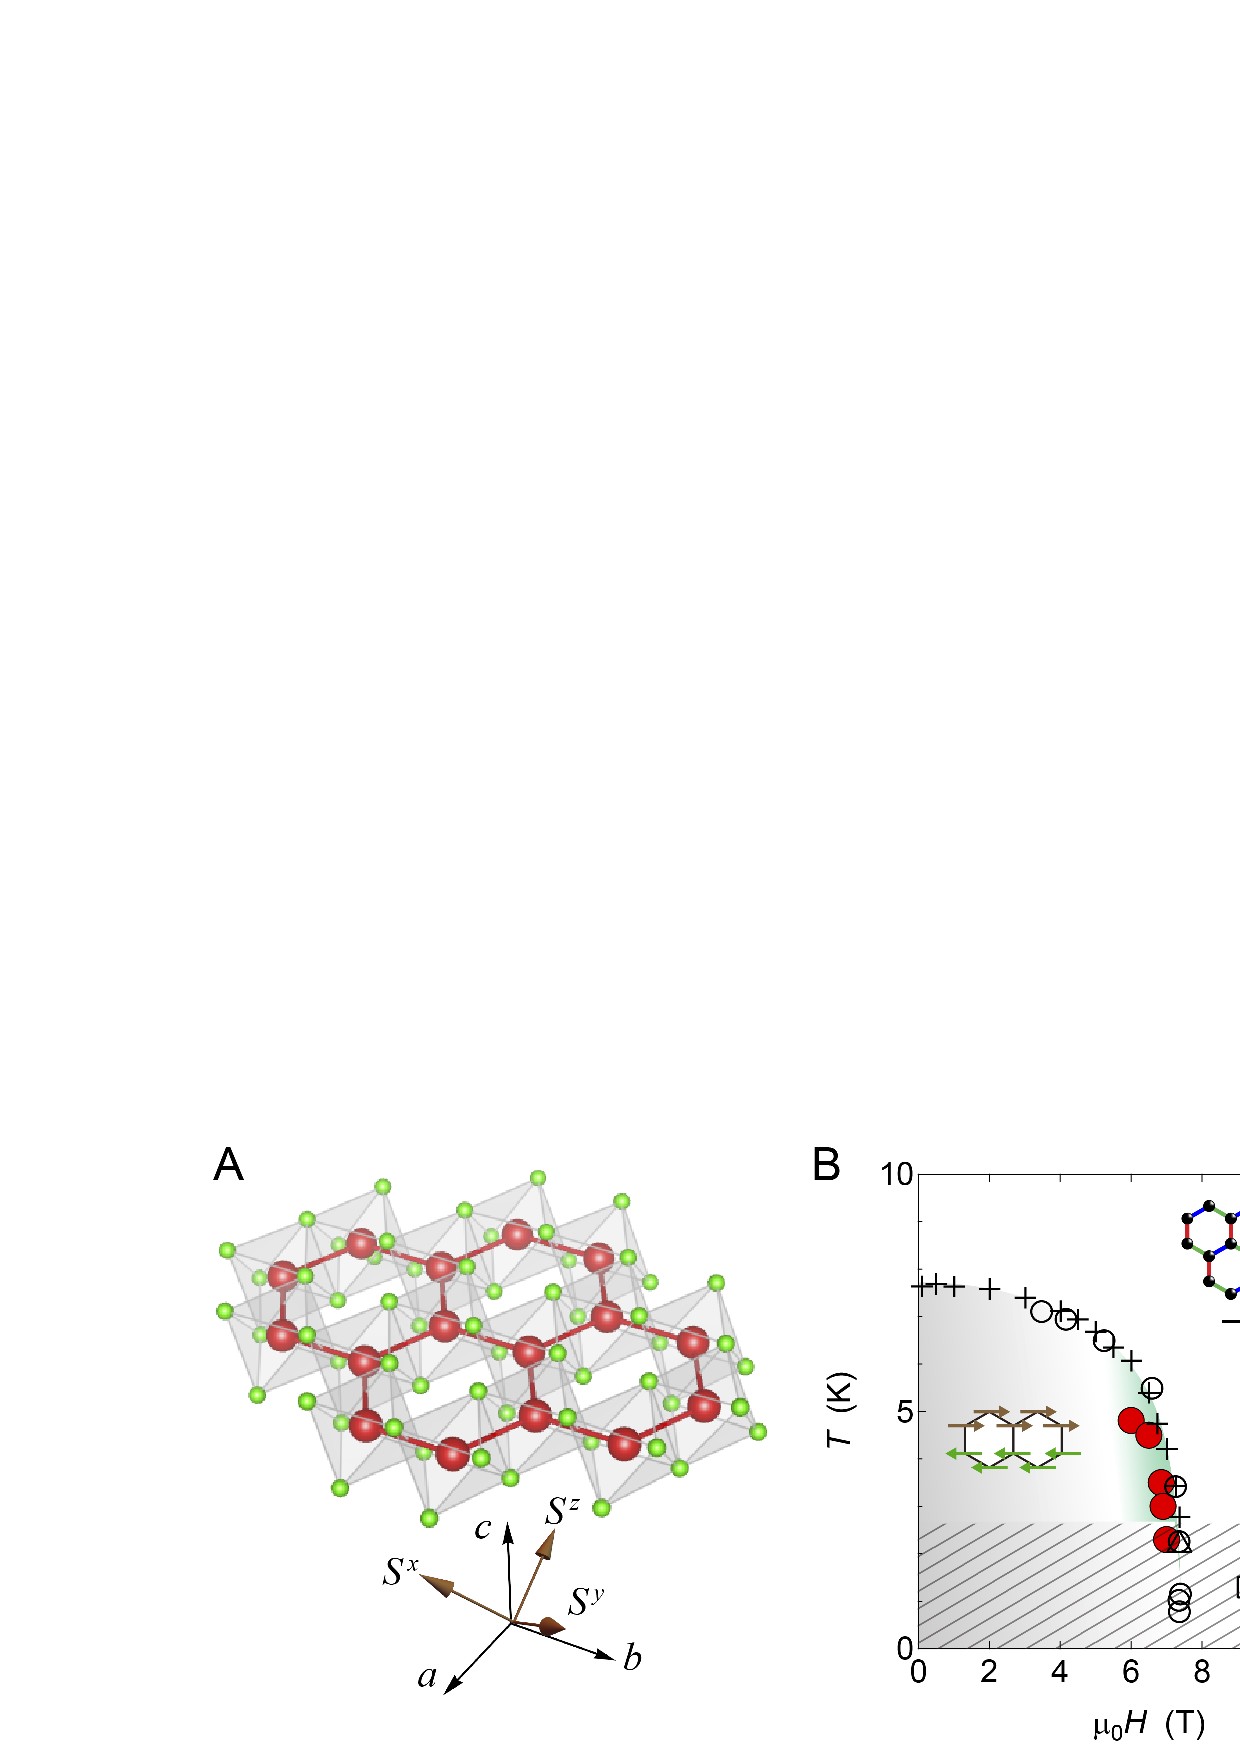
\includegraphics[width= 0.6\textwidth]{images/CH3/Fig1.png}
  \caption{ The honeycomb lattice of ruthenium atoms in red and the chlorine atoms in green. The axis $S^x,S^y, S^z$ is the basis $\bf{\hat{x}},\bf{\hat{y}},\bf{\hat{z}}$. Figure extracted from \cite{yokoi2020halfinteger}.  }
  \label{fig:3-yokoi}
  \end{figure}
  
  


%\begin{figure}[h]
%    \centering
%    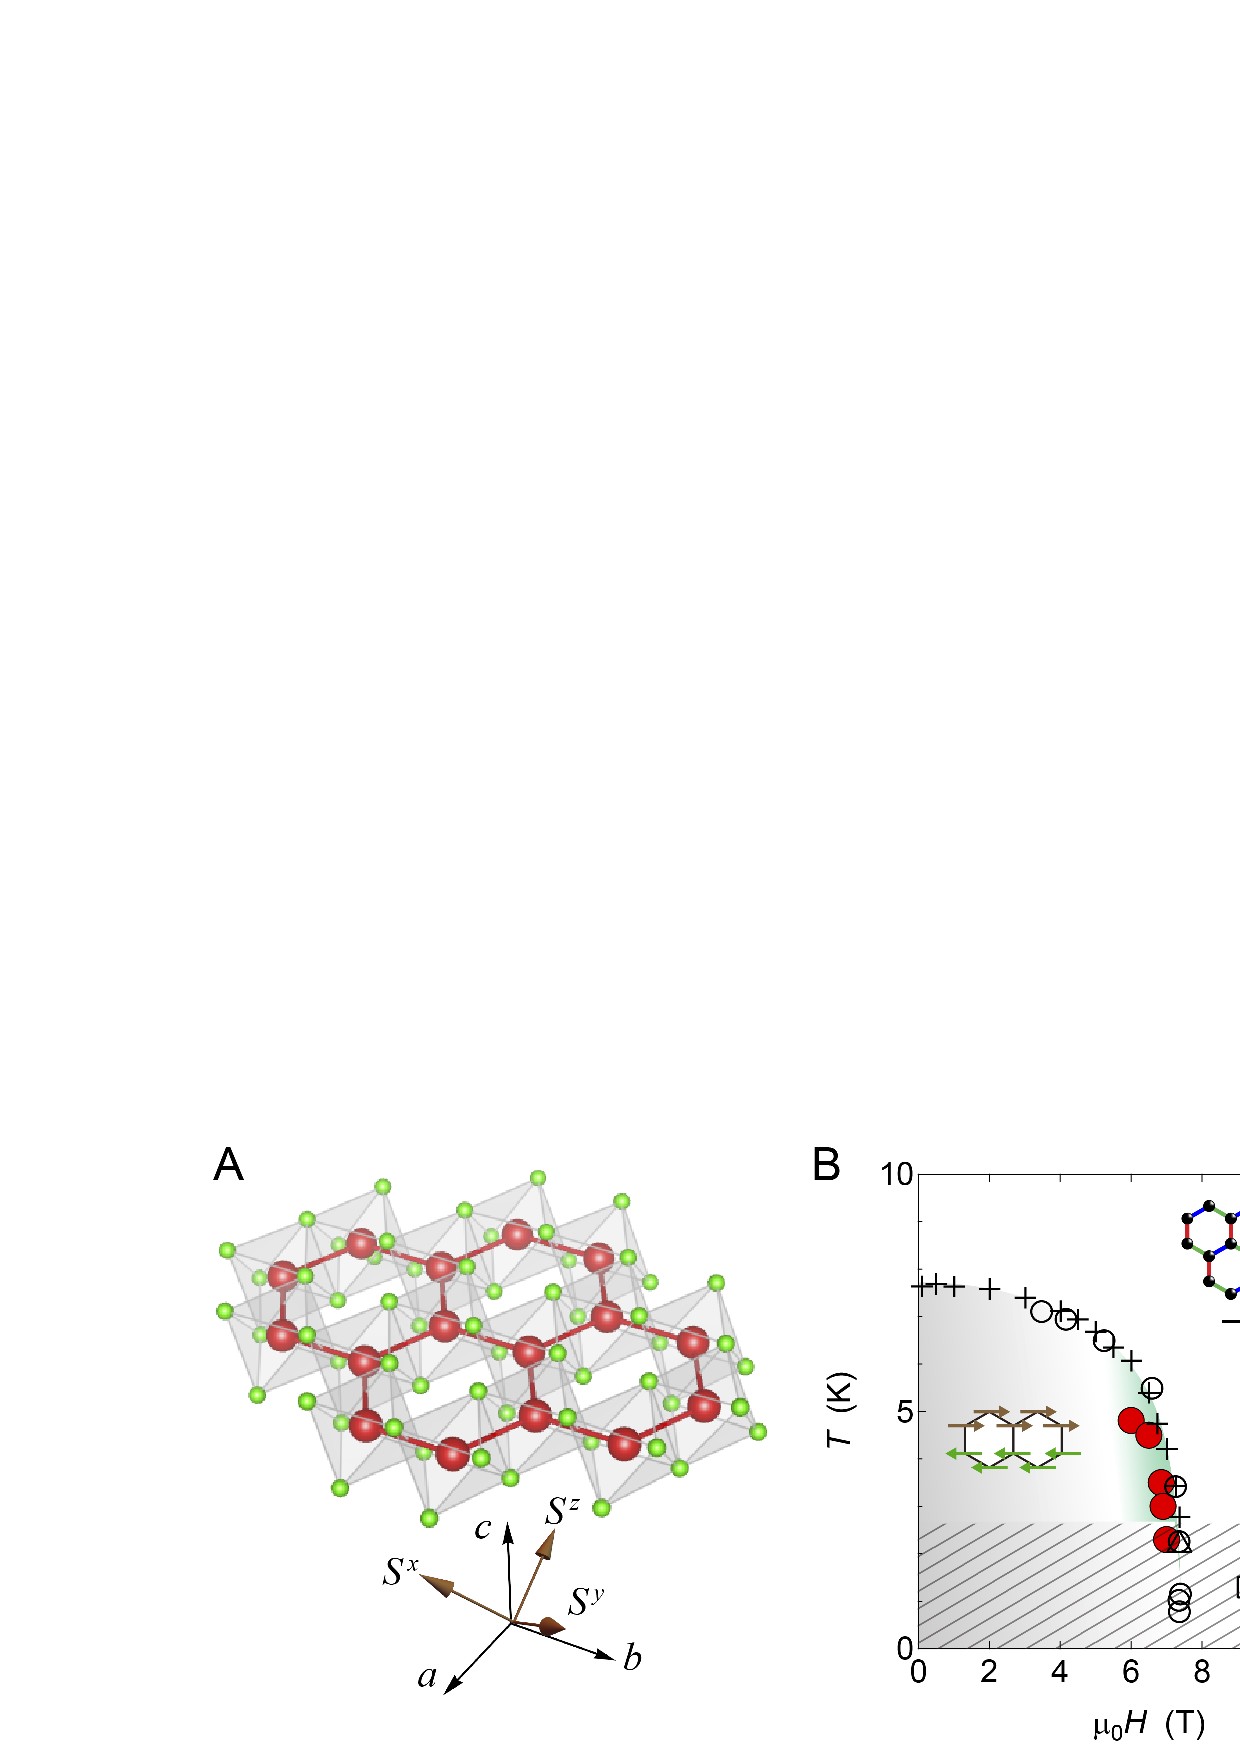
\includegraphics[width= 0.5\textwidth]{images/CH3/Fig1.png}
%    \caption{Lattice structure of \acrshort{rucl} including the Chlorine octahedron.}
%%    \label{fig:3-rucl6}
%\end{figure}

Even though $\bf{a}$ and $\bf{b}$ are always defined in the plane in the literature, their directions vary from author to author. I am following the definitions used in \cite{yokoi2020halfinteger,Liu_2018} in which $\bf{b}$ is taken to be parallel to the z-link and $\bf{a}= \bf{b} \times \bf{c} $. 

I note that the axes are respectively orthogonal to the corresponding bonds. For example, the \textit{z} type bond is in the $(1,-1,0)$ direction, while the $z$-direction is along $(0,0,1)$. If $[\gamma\text{-link}]$ denotes the unit vector in the direction of a $\gamma$ type bond, in terms of the basis these vectors are 
\begin{align}
    [x\text{-link}] \; & = \; \frac{1}{\sqrt{2}} \, \left( \, \hat{y} \; - \; \hat{z} \, \right) \; , \\
    [y\text{-link}] \; & = \; \frac{1}{\sqrt{2}} \, \left( \, \hat{z} \; - \; \hat{x} \, \right) \; , \\
    [z\text{-link}] \; & = \; \frac{1}{\sqrt{2}} \, \left( \, \hat{x} \; - \; \hat{y} \, \right) \; , 
\end{align}
see Ref.\cite{Liu_2018} for a picture of all vectors in a unit sphere.



\section{Edge modes - the microscopic Hamiltonian}

The Hamiltonian is a sum of local terms. For the terms that happen in the bulk, the Hamiltonian is the same as \eqref{2-Ham-mag}. The Hamiltonian differs at the edge, in which it is considered the Zeeman coupling $-\sum_{j} \bm{\sigma}_j \cdot \bf{h}$ without approximations. % In particular, the zigzag edge has a peculiarity that, after rewriting the spin as Majorana fermions \eqref{eq:2-maj-t}, all $b^x$ and $b^y$ are coupled into the gauge fields $u$, while $b^z$ at the edge will remain uncoupled to others $b^\alpha$ field. The dynamic of these fields appears due to the Zeeman interaction. 
The Hamiltonian is
\begin{equation}
    H \; = \; \; -  \, J \sum_{\, \langle j,k \rangle_{\alpha} }  \, \im \, \hat{u}_{jk} \, c_j c_k    \; - \; \kappa  \sum_{ \, \langle \langle i,k \rangle \rangle }   \, \im \hat{u}_{ij}\hat{u}_{jk} \,c_i c_k  \; - \; \sum_{j \in \text{Edge}} \im h_{z}b_{j}^{z} c_{j} \; . \label{eq:3-H}
\end{equation}
\begin{figure}[t]
  \begin{minipage}{.7\textwidth}
    \centering
    \scalebox{1.3}{\documentclass{standalone}  
\usepackage{tikz,comment}
\usepackage[active,tightpage]{preview}
\PreviewEnvironment{tikzpicture}
\setlength\PreviewBorder{1pt}
%%%
\usetikzlibrary{arrows} 





\begin{document}
% Define the layers to draw the diagram
\pgfdeclarelayer{background}
\pgfdeclarelayer{foreground}
\pgfsetlayers{background,main,foreground}


\def \h { 0.57735026918}  % 1/sqrt(3) comprimento  y  de uma celula                                     even (White, 2y) to odd (black ,2y+1) 
\def \d { 0.28867513459}  % 1/ 2 sqrt(3)  distancia  y  entre celulas                                   odd (black , 2y-1) to even (white , 2y)
\def \c { 0.5}           % 1/2 distancia  x  entre celulas  
\def \v { 0.86602540378 }  % sqrt(3)/ 2   distancia  y  de duas celulas                                   odd-odd or even-even 


\def \mar {0.2}  % margin for the clip

\def \l {7}         %horizontal length

\begin{tikzpicture}[>=latex]






\clip (-\mar+1-.1,  \v -2*\d -2*\d-2*\v -\mar -.5) rectangle (\l+\mar+1+.1,\v+\mar+1);

\foreach \a in {0,...,\l}{
  %      \draw[draw=blue!80!black, line width=0.40mm] ( \c +\a, \v  )-- ( \c+\a, \v + \c);
        \draw[draw=blue!80!black, line width=0.40mm] ( \c+\a, -\d )-- ( \c+\a, -\d -\v+\d);
  %      \draw[draw=blue!80!black, line width=0.40mm] ( \c +\a, \v -\c-2*\d-2*\v )-- ( \c+\a, \v -\c -\c-2*\d-2*\v);
}


\draw[<->,draw=orange!80!black, line width=0.40mm] (-\mar+1+.2,  \v+\mar+ 0.2) --  (\l+\mar+1-.7,\v+\mar+0.2);
\node at ( 3.5+.55, -\d - .15+2) [right] { \scriptsize \textcolor{orange!75!black}{\small $\ell_x$}   };

\foreach \b in {-1,0}{    
    \foreach \a in {1,3,...,\l} {
        \draw[draw=red!80!black, line width=0.40mm] ( \a , -\d +\v+ 2*\v*\b    ) -- ( \a -\c, -\d +\v+ 2*\v*\b   +\d );
        \draw[draw=green!80!black, line width=0.40mm] (\a , -\d +\v+ 2*\v*\b - \v+\d )-- ( \a -\c,  -\d +\v+ 2*\v*\b - \v);
            }   
}


\foreach \b in {-1,0}{    
    \foreach \a in {1,3,...,\l} {        
        \node[circle, fill=white, draw=black, line width=0.40mm, inner sep=2pt, minimum size=2pt] (W1\b\a) at ( \a , -\d +\v+ 2*\v*\b    ) {};
    	\node[circle, fill=black, draw=black, line width=0.40mm, inner sep=2pt, minimum size=2pt] (B2\b\a) at ( \a + \c, \v + 2*\v*\b   ) {};
        \node[circle, fill=white, draw=black, line width=0.40mm, inner sep=2pt, minimum size=2pt] (W3\b\a) at ( \a +1, -\d +\v+ 2*\v*\b    ) {};
    	\node[circle, fill=black, draw=black, line width=0.40mm, inner sep=2pt, minimum size=2pt] (B4\b\a) at ( \a +1, -\d +\v+ 2*\v*\b - \v+\d)  {};
    	\node[circle, fill=white, draw=black, line width=0.40mm, inner sep=2pt, minimum size=2pt] (W5\b\a) at ( \a -\c + 1, -\d +\v+ 2*\v*\b - \v) {};  	
    	\node[circle, fill=black, draw=black, line width=0.40mm, inner sep=2pt, minimum size=2pt] (B6\b\a) at  ( \a , -\d +\v+ 2*\v*\b - \v+\d ) {};

    	\node[circle, fill=black, draw=black, line width=0.40mm, inner sep=2pt, minimum size=2pt] (B2r\b\a) at ( \a + \c+1, -\d +\v+ 2*\v*\b+\d   ) {}; 
    	\node[circle, fill=white, draw=black, line width=0.40mm, inner sep=2pt, minimum size=2pt] (W5r\b\a) at ( \a -\c + 2, -\d +\v+ 2*\v*\b - \v) {};    	
    	
    }   
}

\foreach \b in {-1,0}{    
    \foreach \a in {1,3,...,\l} { 
        \draw[draw=green!80!black, line width=0.40mm] (B2\b\a)-- (W1\b\a);
        \draw[draw=red!80!black, line width=0.40mm] (B2\b\a)--(W3\b\a);
        \draw[draw=blue!80!black, line width=0.40mm] (W1\b\a)--(B6\b\a);
 %       \draw[draw=red!80!black, line width=0.40mm] (W1\b\a)-- ( \a -\c, -\d +\v+ 2*\v*\b   +\d );
        \draw[draw=green!80!black, line width=0.40mm] (B2r\b\a)-- (W3\b\a);        
        \draw[draw=blue!80!black, line width=0.40mm] (W3\b\a)--(B4\b\a);       
        \draw[draw=red!80!black, line width=0.40mm] (W5\b\a)--(B6\b\a);        
        \draw[draw=green!80!black, line width=0.40mm] (B4\b\a)-- (W5\b\a);
        \draw[draw=red!80!black, line width=0.40mm] (W5r\b\a)--(B4\b\a); 
%        \draw[draw=green!80!black, line width=0.40mm] (B6\b\a)-- ( \a -\c, 2*\v*\b   - \d);
            }   
}


\end{tikzpicture}
\end{document}}
    %\caption{Caption}
    %\label{fig:3-lattice}
  \end{minipage}%
  \begin{minipage}{.3\textwidth}
    \centering
    \scalebox{1.3}{\documentclass{standalone}  
\usepackage{tikz,comment}
\usepackage[active,tightpage]{preview}
\PreviewEnvironment{tikzpicture}
\setlength\PreviewBorder{1pt}
%%%
\usetikzlibrary{arrows} 





\begin{document}
% Define the layers to draw the diagram
\pgfdeclarelayer{background}
\pgfdeclarelayer{foreground}
\pgfsetlayers{background,main,foreground}


\def \h { 0.57735026918}  % 1/sqrt(3) comprimento  y  de uma celula                                     even (White, 2y) to odd (black ,2y+1) 
\def \d { 0.28867513459}  % 1/ 2 sqrt(3)  distancia  y  entre celulas                                   odd (black , 2y-1) to even (white , 2y)
\def \c { 0.5}           % 1/2 distancia  x  entre celulas  
\def \v { 0.86602540378 }  % sqrt(3)/ 2   distancia  y  de duas celulas                                   odd-odd or even-even 


\def \mar {0.2}  % margin for the clip

\def \l {7}         %horizontal length

\begin{tikzpicture}[>=latex]





\draw[<-,draw=cyan!80!black, line width=0.40mm] (2+.6, -4*\d -\v -.15 ) --  (2+.6,\v+.15);
\node at ( 2.65, -2*\d ) [right] { \scriptsize \textcolor{cyan!75!black}{\small $\ell_y$}   };
\clip (-\mar+1+ \c-.75,  \v -2*\d -2*\d-2*\v -\mar -.5) rectangle (\mar+2+.75+.3,\v+\mar+1);

\foreach \a in {1}{
  %      \draw[draw=blue!80!black, line width=0.40mm] ( \c +\a, \v  )-- ( \c+\a, \v + \c);
        \draw[draw=blue!80!black, line width=0.40mm] ( \c+\a, -\d )-- ( \c+\a, -\d -\v+\d);
  %      \draw[draw=blue!80!black, line width=0.40mm] ( \c +\a, \v -\c-2*\d-2*\v )-- ( \c+\a, \v -\c -\c-2*\d-2*\v);
}


\foreach \b in {-1,0}{    
    \foreach \a in {1} {
   %     \draw[draw=red!80!black, line width=0.40mm] ( \a , -\d +\v+ 2*\v*\b    ) -- ( \a -\c, -\d +\v+ 2*\v*\b   +\d );
  %      \draw[draw=green!80!black, line width=0.40mm] (\a , -\d +\v+ 2*\v*\b - \v+\d )-- ( \a -\c,  -\d +\v+ 2*\v*\b - \v);
            }   
}


\foreach \b in {-1,0}{    
    \foreach \a in {1} {    
    	\node[circle, fill=black, draw=black, line width=0.40mm, inner sep=2pt, minimum size=2pt] (B2\b\a) at ( \a + \c, \v + 2*\v*\b   ) {};
        \node[circle, fill=white, draw=black, line width=0.40mm, inner sep=2pt, minimum size=2pt] (W3\b\a) at ( \a +1, -\d +\v+ 2*\v*\b    ) {};
    	\node[circle, fill=black, draw=black, line width=0.40mm, inner sep=2pt, minimum size=2pt] (B4\b\a) at ( \a +1, -\d +\v+ 2*\v*\b - \v+\d)  {};
    	\node[circle, fill=white, draw=black, line width=0.40mm, inner sep=2pt, minimum size=2pt] (W5\b\a) at ( \a -\c + 1, -\d +\v+ 2*\v*\b - \v) {};  	
 %   	\node[circle, fill=black, draw=black, line width=0.40mm, inner sep=2pt, minimum size=2pt] (B6\b\a) at  ( \a , -\d +\v+ 2*\v*\b - \v+\d ) {};
    %	\node[circle, fill=black, draw=black, line width=0.40mm, inner sep=2pt, minimum size=2pt] (B2r\b\a) at ( \a + \c+1, -\d +\v+ 2*\v*\b+\d   ) {}; 
%    	\node[circle, fill=white, draw=black, line width=0.40mm, inner sep=2pt, minimum size=2pt] (W5r\b\a) at ( \a -\c + 2, -\d +\v+ 2*\v*\b - \v) {};    		
    }   
}


        \draw[draw=red!80!black, line width=0.40mm] (B201)--(W301);
  %      \draw[draw=green!80!black, line width=0.40mm] (B2r01)-- (W301);        
        \draw[draw=blue!80!black, line width=0.40mm] (W301)--(B401);       
  %      \draw[draw=red!80!black, line width=0.40mm] (W501)--(B601);        
        \draw[draw=green!80!black, line width=0.40mm] (B401)-- (W501);
        \draw[draw=red!80!black, line width=0.40mm] (B2-11)--(W3-11);
    %    \draw[draw=green!80!black, line width=0.40mm] (B2r-11)-- (W3-11);        
        \draw[draw=blue!80!black, line width=0.40mm] (W3-11)--(B4-11);       
     %   \draw[draw=red!80!black, line width=0.40mm] (W5-11)--(B6-11);        
        \draw[draw=green!80!black, line width=0.40mm] (B4-11)-- (W5-11);


\end{tikzpicture}
\end{document}}
    %\caption{Caption}
    %\label{fig:3-lattice-FT}
  \end{minipage}
  \caption{(Left) The  lattice for $\ell_x = 14$ and $\ell_y=8$; the lattice continues periodically in the $x$ direction, but it is finite in the $y$ direction. (Right) After Fourier transforming in the $x$ direction, the effective lattice becomes an open chain (1D lattice). }
  \label{fig:3-lattice}
  \end{figure}
Choosing the standard gauge \eqref{eq:2-gauge-fix} the system is then invariant by discrete translations of $\bf{n}_1-\bf{n}_2=(1,0)$. 

Let suppose that the horizontal length (in the periodic direction) of the system is finite $\ell_x$ and in the vertical direction is $\ell_y$ with both even numbers.  The schematic representation is shown in  figure \ref{fig:3-lattice}.  After Fourier transforming in the $x$ direction the Majoranas are transformed into complex fields $b_{q , y}$ and $c_{q,y}$. %which for the $c$ fermions the integer index $y$ indicates the vertical position,% and is even or odd if the Majorana fermions was defined at the lattice % while for $b$ it take two values $1$ or $\ell_y$ depending if the term is at the upper edge ($\mathcal{L}_{\text{O}}$, colour black in the figure) or at the lower edge ($\mathcal{L}_{\text{E}}$, colour white).
\begin{align}
     \tilde{A}_{y_1y_2}(q)  \; &= \;  \sum_{x} \, e^{\im qx} A_{0y_1,xy_2} \; \label{eq:3-fourier-t} , \\[6pt]
    c_{q,y} \; &= \; \frac{1}{\sqrt{2\ell_x}} \, \sum_{x} \, e^{- \im q x} c_{xy} \; ,  \label{eq:3-fourier-t-c}  \\[6pt]
    b^{z}_{q,y} \; &= \; \frac{1}{\sqrt{2\ell_x}} \, \sum_{x} \, e^{- \im q x} b^{z}_{xy} \; , \quad \text{for } y = 0 \text{ or } \ell_{y}+1 \, .
\end{align}
The momentum is discretized in to the \acrlong{bz}: $\text{BZ}= \big\{  \frac{2\pi n}{\ell_x} \, \Big\vert \,  n = -\frac{\ell_x}{2}+1 , $ $...,\frac{\ell_x}{2} \big\}$. The normalization factors are chosen so that $c_{q,y}$ and $ b^{z}_{q,y}$ obeys the usual anticommutation relations for complex fermions when restricted to positive momentum. The restriction is called \acrfull{hbz} and it is $\frac{1}{2}\text{BZ}= \left\{  \frac{2\pi}{\ell_x}, \frac{4\pi}{\ell_x}, ,...,\pi  \right\}$. For example, with this normalization, the inverse Fourier transform for the Majorana operators is
\begin{align}
    c_{xy} \; &= \; \sqrt{\frac{2}{\ell_x}} \, \sum_{q \in \text{BZ}} \, e^{\im q x} c_{q,y}  \; = \;  \sqrt{\frac{2}{\ell_x}} \, \sum_{q \in \frac{1}{2}\text{BZ}} \, \Big( \,e^{\im q x} c_{q,y} \, + \, e^{-\im q x} c_{q,y}^{\dagger} \, \Big)\; . \label{eq:3-inverse-fourier}
\end{align}


The Hamiltonian obtained after the Fourier transform is 
\begin{equation}
    H \;= \; \sum_{q \in \frac{1}{2}\text{BZ}} \sum_{y_1,y_2 = 0}^{\ell_y+1} \, \im \tilde{A}_{y_1y_2}(q) \, c_{q,y_1}^{\dagger} c_{q,y_2}  \; ,
\end{equation}
with $c_{0} := b_1^z$, $c_{\ell_y+1} := b_{\ell_y}^z$ and $\im A$ is the  $(\ell_y+2)\times(\ell_y+2)$ Hermitean matrix
\begin{equation}
  \im \tilde{A}(q) = 
   \left(
\begin{array}{cccccccccccc}
 0 & i \gamma  & 0 & 0 & 0 & 0 & 0 & 0 & 0 & 0 %& 0 & 0 
 \\
 -i \gamma  & \alpha  & i s & \textcolor{black!60}{-\textcolor{black!60}{\beta}}  & 0 & 0 & 0 & 0 & 0 & 0% & 0 & 0 
 \\
 0 & -i s & -\alpha  & \textcolor{black!60}{i r} & \textcolor{black!60}{\beta}  & 0 & 0 & 0 & 0 & 0% & 0 & 0 
 \\
 0 & \textcolor{black!60}{-\textcolor{black!60}{\beta}}  & \textcolor{black!60}{- i r} & \alpha  & i s & \textcolor{black!60}{-\textcolor{black!60}{\beta}}  & 0 & 0 & 0 & 0% & 0 & 0
 \\
 0 & 0 & \textcolor{black!60}{\beta}  & -i s & -\alpha  & \textcolor{black!60}{i r} & \textcolor{black!60}{\beta}  & 0 & 0 & 0 %& 0 & 0
 \\
 0 & 0 & 0 & \ddots  &  \ddots & \ddots  & \ddots & \ddots  & 0 & 0% & 0 & 0
 \\
 0 & 0 & 0 & 0 & \ddots & \ddots & \ddots  & \ddots &  \ddots  & 0 & % 0 & 0 
 \\%
 %0 & 0 & 0 & 0 & 0 & \textcolor{black!60}{-\textcolor{black!60}{\beta}}  & \textcolor{black!60}{- i r} & \alpha  & i s & \textcolor{black!60}{-\textcolor{black!60}{\beta}}  & 0 & 0 \\ 
% 0 & 0 & 0 & 0 & 0 & 0 & \textcolor{black!60}{\beta}  & -i s & -\alpha  & \textcolor{black!60}{i r} & \textcolor{black!60}{\beta}  & 0 \\
% 0 & 0 &
0 & 0 & 0 & 0 & 0 & \textcolor{black!60}{-\textcolor{black!60}{\beta}}  & \textcolor{black!60}{- i r} & \alpha  & i s & 0 \\
% 0 & 0 &
0 & 0 & 0 & 0 & 0 & 0 & \textcolor{black!60}{\beta}  & -i s & -\alpha  & -i \gamma  \\
% 0 & 0 & 
0 & 0 & 0 & 0 & 0 & 0 & 0 & 0 & i \gamma  & 0 \\
\end{array}
\right) \,  , \label{eq:3-hamiltonian}
%\begin{pmatrix}    c_{k}(1) \\ c_{k}(2) \\c_{k}(3) \\c_{k}(4) \\c_{k}(5)\\ \vdots\\ \vdots \\ c_{k}(-4) \\ c_{k}(-3) \\
%    c_{k}(-2) \\    c_{k}(-1) \\    c_{k}(L) \\\end{pmatrix}
\end{equation}
in which the matrix elements are defined as 
%\begin{align}    \alpha       & = 4  \, \kappa  \, \sin(q) \, ,  \\    \beta        & = 4  \, \kappa  \, \sin(q/2) \, ,  \\    r               & = 2  J  \,  ,   \\    s               & = -4   \, J \, \cos(q/2)   \, , \quad \text{and} \\      \gamma         &   = - 2 h_{z} \;. \end{align}
\begin{align}
    \alpha       & = 2\, \kappa  \, \sin(q) \, ,  \\
    \beta        & = 2  \, \kappa  \, \sin(q/2) \, ,  \\
    r               & =   J  \,  ,   \\
    s               & = -2   \, J \, \cos(q/2)   \, , \\  
    \gamma          &   = - h_{z} \;.
\end{align}
The indices for matrix elements of $\tilde{A}(q)$ are allowed to take values between $0$ and $\ell_y+1$. The zeroth row and column are associated with the $b^z$ at $y=1$, as well as the last ($\ell_y+1$-th) row and column are associated with $b^z$ at $y=\ell_y$. With this terminology, the sites with $y=0$ or $y=\ell_y+1$ can be thought of as fictitious new two sites in which the $b$ fermions live.  

The couplings $\alpha$ and $s$ acts inside the unit cell, while $\beta$ and $r$ couples different unit cells. 
The $r$ and $s$ terms are directly understood as a representation of the \acrshort{nn} interaction in \eqref{eq:3-H}, and the $\alpha$ and $\beta$ are representations of the \acrshort{nnn}. Importantly, the $\gamma$ coupling is the Zeeman terms and is the one that couples $b^z$ and $c$ at the edge. That is, for a strong $\gamma$ these modes are hybridized. 

\section{Dispersion of the chiral models}

The spectrum depends on the direction and strength of the applied field. The dependence in the direction of the magnetic field enters on the Hamiltonian by the $\kappa$ dependence as the product of $h_x h_y h_z$. As known from the theory in the bulk, see chapter \ref{ch:2}, when $\kappa$ is zero the spectrum is gapless. For in-plane fields, this happens only in the discrete cases in which $\bf{h}$ is aligned to the bond directions.

 Here and in the following numerical calculations I set $\kappa = h_xh_yh_z$; this choice for proportionality constant $1$ is questionable, the predicted value is much smaller. Nevertheless, for this work this precision will not be relevant. In the calculation, I used a magnetic field of modulo $0.85 \text{ J}$. This value is arbitrary, I choose a high value for the magnetic field to amplify the contrast between different configurations. %Bear in mind that . %very signification gap in the dispersion calculated. % bear in mind that the magnetic field  $0.85$


The energy dispersion of the case in which the magnetic field is in-plane and along the z-link is shown in figure \ref{fig:3-disp-b}. The gapped behavior is in agreement with the experiment \cite{yokoi2020halfinteger} since the Hall conductivity is absent when the magnetic field is parallel to the $\bf{b}$ direction. The same dispersion for the Majorana fermions in the bulk is obtained for the field along the x-link and y-link, i.e. whenever $\kappa =0$.
 \begin{figure}[h]
    \centering
    \includegraphics[width = 0.6 \textwidth]{images/CH3/disp_b.pdf}
    \caption{Magnetic field in the $\bf{b}$ direction with modulus $0.85 \, J$. The gap in the bulk is zero.  Numerical calculation was performed for $\ell_x = \ell_y = 500$, which is large enough to identify the continuum in the thermodynamic limit, and it is represented by the shaded regions. }
    \label{fig:3-disp-b}
\end{figure}
However, the edge modes obtain a non-vanishing dispersion, see figure \ref{fig:3-disp-x}, between $\frac{2\pi}{3} < q < \frac{4\pi}{3}$ for the fields in along the x- or y-link since the  $z$ component of the magnetic field is non-zero in this situation. Nonetheless, the cases in which the magnetic field point in the direction of the bond are rather exceptional cases. The generic configuration happens for $\kappa \neq 0$ and $h^z \neq 0$.

\begin{figure}[t]
    \centering
    \includegraphics[width = 0.6 \textwidth]{images/CH3/disp_x.pdf}
    \caption{Magnetic field out of the plane in the $[x\text{-link}]$ direction.  }
    \label{fig:3-disp-x}
\end{figure}

Changing the direction of the magnetic field away from the bond direction make the bulk modes gapped out. The edge modes continue being gapless, but the Dirac point changes from $q=\frac{2 \pi}{3}$ to $q=0$. This gapped configuration can be seen in figures \ref{fig:3-disp-a} and \ref{fig:3-disp-c}. These two energy dispersions are qualitatively similar but differ in the magnitude of the Majorana gap.

 \begin{figure}[h]
    \centering
        \begin{subfigure}{.5\textwidth}
        \centering
        \includegraphics[width= 1.1\textwidth]{images/CH3/disp_a.pdf}
        \caption{ Magnetic field in the $\bf{a}$ direction.}
        \label{fig:3-disp-a}
    \end{subfigure}%
    \begin{subfigure}{.5\textwidth}
        \centering
        \includegraphics[width= 1.1\textwidth]{images/CH3/disp_c.pdf} 
        \caption{Magnetic field in the $\bf{c}$ direction. }
        \label{fig:3-disp-c}
    \end{subfigure}
\caption{The  Majorana fermions in the bulk are gapped, while the Majoranas modes localized at the edge are gapless. The gray area indicates the bulk spectrum, while the bold black line is for the gapless edge modes. %Dispersion for field in plane in two distinct directions.Numerical calculation for $\ell_x = \ell_y = 500$ 
}
\end{figure} 

%\begin{figure}[hb!]    \centering    \includegraphics[width = 0.65 \textwidth]{images/CH3/disp_a.pdf}    \caption{Magnetic field in the $\bf{a}$ direction with modulus $0.85 \, J$. The bulk is gapped and the edge is gapless. The grey area indicate the bulk spectrum, while the bold black line is the gapless edge modes. }     \label{fig:3-disp-a} \end{figure}









The conclusion is that, as the direction of the magnetic field changes, the value for the gap oscillates going through zero along the lines where $h_xh_yh_z=0$ and increases in some monotonic way with the absolute value of $h_xh_yh_z$. This result is in complete agreement with the experiments \cite{yokoi2020halfinteger, tanaka2020}.


The sign of $h_xh_yh_z$, $\text{sgn}(h_xh_yh_z)$, for field $\bf{h}$ merely determines if the edge mode has positive or negative chirality, and the spectrum is equivalent. % From the figure cannot be seen but can be shown that the chiral edge modes have opposite chirality to the ones in the figures  \ref{fig:3-disp-a}  and \ref{fig:3-disp-c}, which cannot conclude just with the figure. 
As long as the magnetic field does not cross the lines where $h_xh_yh_z=0$, all octants in the $h$ space are equivalent.  %Lets consider the magnetic field in the first octant of the $h_xh_yh_z$-space. That is, consider that $h_x,h_y,h_z \geq 0$.

This calculation shows that the edge modes have linear dispersion in low energies, which allow me to define the two modes as left- and right-movers around $q=0$.  The velocity for these modes will be calculated in chapter \ref{ch:5}.

In this chapter, I established the theory that will be the base for the following chapters. Here, I have computed the microscopic Hamiltonian for a pure \acrshort{kqsl} in a geometry periodic in one direction and open in the other. In the next chapter, I will consider further interactions on this theory.



%\begin{figure}[b]% \centering     \includegraphics[width = 0.65 \textwidth]{images/CH3/disp_c.pdf}     \caption{Magnetic field out of the plane in the $\bf{c}$ direction.  }     \label{fig:3-disp-c} \end{figure}
%\begin{figure}[h]
%  \begin{minipage}{.5\textwidth}
%    \centering
%%% \end{minipage}%
  %\begin{minipage}{.5\textwidth}
  %  \centering
  %  \scalebox{1.3}{\documentclass{standalone}  
\usepackage{tikz,comment}
\usepackage[active,tightpage]{preview}
\PreviewEnvironment{tikzpicture}
\setlength\PreviewBorder{1pt}
%%%
\usetikzlibrary{arrows} 





\begin{document}
% Define the layers to draw the diagram
\pgfdeclarelayer{background}
\pgfdeclarelayer{foreground}
\pgfsetlayers{background,main,foreground}


\def \h { 0.57735026918}  % 1/sqrt(3) comprimento  y  de uma celula                                     even (White, 2y) to odd (black ,2y+1) 
\def \d { 0.28867513459}  % 1/ 2 sqrt(3)  distancia  y  entre celulas                                   odd (black , 2y-1) to even (white , 2y)
\def \c { 0.5}           % 1/2 distancia  x  entre celulas  
\def \v { 0.86602540378 }  % sqrt(3)/ 2   distancia  y  de duas celulas                                   odd-odd or even-even 


\def \mar {0.2}  % margin for the clip

\def \l {7}         %horizontal length

\begin{tikzpicture}[>=latex]





\draw[<-,draw=cyan!80!black, line width=0.40mm] (2+.6, -4*\d -\v -.15 ) --  (2+.6,\v+.15);
\node at ( 2.65, -2*\d ) [right] { \scriptsize \textcolor{cyan!75!black}{\small $\ell_y$}   };
\clip (-\mar+1+ \c-.75,  \v -2*\d -2*\d-2*\v -\mar -.5) rectangle (\mar+2+.75+.3,\v+\mar+1);

\foreach \a in {1}{
  %      \draw[draw=blue!80!black, line width=0.40mm] ( \c +\a, \v  )-- ( \c+\a, \v + \c);
        \draw[draw=blue!80!black, line width=0.40mm] ( \c+\a, -\d )-- ( \c+\a, -\d -\v+\d);
  %      \draw[draw=blue!80!black, line width=0.40mm] ( \c +\a, \v -\c-2*\d-2*\v )-- ( \c+\a, \v -\c -\c-2*\d-2*\v);
}


\foreach \b in {-1,0}{    
    \foreach \a in {1} {
   %     \draw[draw=red!80!black, line width=0.40mm] ( \a , -\d +\v+ 2*\v*\b    ) -- ( \a -\c, -\d +\v+ 2*\v*\b   +\d );
  %      \draw[draw=green!80!black, line width=0.40mm] (\a , -\d +\v+ 2*\v*\b - \v+\d )-- ( \a -\c,  -\d +\v+ 2*\v*\b - \v);
            }   
}


\foreach \b in {-1,0}{    
    \foreach \a in {1} {    
    	\node[circle, fill=black, draw=black, line width=0.40mm, inner sep=2pt, minimum size=2pt] (B2\b\a) at ( \a + \c, \v + 2*\v*\b   ) {};
        \node[circle, fill=white, draw=black, line width=0.40mm, inner sep=2pt, minimum size=2pt] (W3\b\a) at ( \a +1, -\d +\v+ 2*\v*\b    ) {};
    	\node[circle, fill=black, draw=black, line width=0.40mm, inner sep=2pt, minimum size=2pt] (B4\b\a) at ( \a +1, -\d +\v+ 2*\v*\b - \v+\d)  {};
    	\node[circle, fill=white, draw=black, line width=0.40mm, inner sep=2pt, minimum size=2pt] (W5\b\a) at ( \a -\c + 1, -\d +\v+ 2*\v*\b - \v) {};  	
 %   	\node[circle, fill=black, draw=black, line width=0.40mm, inner sep=2pt, minimum size=2pt] (B6\b\a) at  ( \a , -\d +\v+ 2*\v*\b - \v+\d ) {};
    %	\node[circle, fill=black, draw=black, line width=0.40mm, inner sep=2pt, minimum size=2pt] (B2r\b\a) at ( \a + \c+1, -\d +\v+ 2*\v*\b+\d   ) {}; 
%    	\node[circle, fill=white, draw=black, line width=0.40mm, inner sep=2pt, minimum size=2pt] (W5r\b\a) at ( \a -\c + 2, -\d +\v+ 2*\v*\b - \v) {};    		
    }   
}


        \draw[draw=red!80!black, line width=0.40mm] (B201)--(W301);
  %      \draw[draw=green!80!black, line width=0.40mm] (B2r01)-- (W301);        
        \draw[draw=blue!80!black, line width=0.40mm] (W301)--(B401);       
  %      \draw[draw=red!80!black, line width=0.40mm] (W501)--(B601);        
        \draw[draw=green!80!black, line width=0.40mm] (B401)-- (W501);
        \draw[draw=red!80!black, line width=0.40mm] (B2-11)--(W3-11);
    %    \draw[draw=green!80!black, line width=0.40mm] (B2r-11)-- (W3-11);        
        \draw[draw=blue!80!black, line width=0.40mm] (W3-11)--(B4-11);       
     %   \draw[draw=red!80!black, line width=0.40mm] (W5-11)--(B6-11);        
        \draw[draw=green!80!black, line width=0.40mm] (B4-11)-- (W5-11);


\end{tikzpicture}
\end{document}}
  %\end{minipage}
  %\caption{}
  %\label{fig:3-lattice}
  %\end{figure}
  
  
  
% \begin{figure}[h]    \begin{minipage}{.5\textwidth}     \centering       \includegraphics[width = 0.9 \textwidth]{images/CH3/disp_a.pdf}  \end{minipage}%  \begin{minipage}{.5\textwidth} \centering   \includegraphics[width = 0.9 \textwidth]{images/CH3/disp_c.pdf}   \end{minipage}    \caption{(Left) Magnetic field in the $\bf{a}$ direction with modulus $0.85 \, J$. The bulk is gapped and the edge is gapless.  (Right) Magnetic field in the $\bf{b}$ direction with modulus $0.85 \, J$. The gap in the bulk is zero.     }  \label{fig:3-disp-ab}   \end{figure}
  

  




\chapter{Majorana fermions %Mean Field for the Majoranas %gapless modes 
in linear defects}
\label{ch:4}
\begin{comment}
\textcolor{red!40!black}{
In this important chapter I want the explain how Majoranas are localized in defects and to calculate in mean-field approximation the phase diagram. 
\begin{itemize}
    \item Brief explanation of how linear defects may be formed in the \acrshort{rucl} by stacking faults; [Need to study more! also : look for numerical values for the coupling and dependence with the distance];
    \item Consider a local experiment near the defect as two adjacent Kitaev materials being proximate. The (homogeneous) coupling $\tilde{J}$ between the two material describe a (apparently second order) phase transition from a non-interacting to a hybridized one at finite critical coupling $\tilde{J}_c$. 
    \item Perform the calculation in mean-field approximation: set two homogeneous order parameter, Fourier transform in x-direction, perform a unitary transformation, %(analytically unknown,  but numerically know)
     calculate self-consistently (numerically) the order parameters, find the phase diagram ( $\tilde{J}_c$ as function of $h$);
\end{itemize}
As long as the defect is \say{wider enough}, so that the effective coupling $\tilde{J}$ is smaller than $\tilde{J}_c$, it will harbors localized gapless chiral Majorana fermions.}
\pagebreak 
\end{comment}
%%%%%%%%%%%%%%%%%%%%%%%%%%%%%%%%%%%%%%%%%%%%%%%%%%%%%%%%%%%%%%%%%%%%%%%%%%%


The fundamentals for the Kitaev model were described in the previous chapters, and now I will start the description of the defects. This work does not intend to be a study of all types of defects in Kitaev material. %Actually, the much more humble goal of this work consists of study a particular type of defect.
%Majorana modes in the gapped (B) phase lives in the edge of the material. %The defects that I am interested are those whose mimics a edge, but inside the bulk. Even beside this types of defects, I will only study one simple case in which the defect happens in a straight line along the $a$ direction as shown in \ref{fig:4-defect}.
In this work I will focus on a particular the of one-dimensional defect characterized by broken bonds on a straight line along the $a$ direction as show in the figure \ref{fig:4-defect}.
The effect of dislocations and string defects in the $A$ phase was studied in Ref. \cite{Olga_2014}. %In contrast, I am interested in defects in the $B$ phase. 
For a recent study of point defect (vacancies) in \acrshort{kqsl} see\cite{kao2020vacancyinduced}. 

\begin{figure}[t]  
    \centering
    %\framebox[.6\textwidth][r]{\includegraphics[width=0.8\textwidth ]{Tikz/CH4/T:4-Defect} }
    % \framebox[.8\textwidth][r]{\scalebox{1.15}{\input{Tikz/CH4/T:4-Defect-v2} }}% could also use \makebox
    \hspace*{-11mm}
    \scalebox{1.2}{\documentclass{standalone}  
\usepackage{tikz,comment}
\usepackage[active,tightpage]{preview}
\PreviewEnvironment{tikzpicture}
\setlength\PreviewBorder{1pt}
%%%
\usetikzlibrary{arrows} 





\begin{document}
% Define the layers to draw the diagram
\pgfdeclarelayer{background}
\pgfdeclarelayer{foreground}
\pgfsetlayers{background,main,foreground}


\def \h { 0.57735026918}  % 1/sqrt(3) comprimento  y  de uma celula                                     even (White, 2y) to odd (black ,2y+1) 
\def \d { 0.28867513459}  % 1/ 2 sqrt(3)  distancia  y  entre celulas                                   odd (black , 2y-1) to even (white , 2y)
\def \c { 0.5}           % 1/2 distancia  x  entre celulas  
\def \v { 0.86602540378 }  % sqrt(3)/ 2   distancia  y  de duas celulas                                   odd-odd or even-even 


\def \mar {0.2}  % margin for the clip

\def \l {11}         %horizontal length
\def \lm {\l-1}
\def \lmm {\l-2}

\begin{tikzpicture}[>=latex]





 \clip (-\mar+1, \v +\h -5*\v  -\mar ) rectangle (\l+\mar+\c-1, \v +2*\v +\mar);
% \clip (-\mar+1,  \v -2*\d -2*\d-2*\v -\mar ) rectangle (\l+\mar+1,\v+\mar);



%%%%%%%%%%%% For the interaction between the edges of the defect %%%%%%%%%%%%%%%%%%%%
\foreach \b in {-1}{
    \foreach \a in {1,2,3,4,5,6,7,8,9,10}{
        \draw[draw=blue!60!white, dashed, line width=0.40mm] ( \c +\a, \v +2*\v*\b  )--( \a , -\d +\v    );
    }
}
\node at ( 5.74 , -.10  ) {\textcolor{blue!60!white}{$\tilde{J}$}};
%%%%%%%%%%%%%%%%%%%%%%%%%%%%%%%%%%%%%%%%%%%%%%%%%%%




\foreach \b in {-3,-2,0,1}{
    \foreach \a in {0,...,\l}{
            \draw[draw=blue!80!black, line width=0.40mm] ( \c +\a, \v +2*\v*\b  )-- ( \c+\a, \v + \h+2*\v*\b );
    }
}
%\foreach \b in {-1}{    \foreach \a in {1,2,\lmm,\lm,\l}{            \draw[draw=blue!80!black, line width=0.40mm] ( \c +\a, \v +2*\v*\b  )-- ( \c+\a, \v + \h+2*\v*\b );    }}


\foreach \b in {-2,-1,0,1}{    
    \foreach \a in {1,3,...,\l} {
        \draw[draw=green!80!black, line width=0.40mm] ( \a , -\d +\v+ 2*\v*\b    ) -- ( \a -\c, -\d +\v+ 2*\v*\b   +\d );
            }   
}
\foreach \b in {-2,-1,1}{    
    \foreach \a in {1,3,...,\l} {
        \draw[draw=red!80!black, line width=0.40mm] (\a , -\d +\v+ 2*\v*\b - \v+\d )-- ( \a -\c,  -\d +\v+ 2*\v*\b - \v);
            }   
}

%\foreach \b in {0}{        \foreach \a in {1,\l} {        \draw[draw=red!80!black, line width=0.40mm] (\a , -\d +\v+ 2*\v*\b - \v+\d )-- ( \a -\c,  -\d +\v+ 2*\v*\b - \v);            }   }

\foreach \b in {-2,-1,0,1}{    
    \foreach \a in {1,3,...,\l} {        
        \node[circle, fill=white, draw=black, line width=0.40mm, inner sep=2pt, minimum size=2pt] (W1\b\a) at ( \a , -\d +\v+ 2*\v*\b    ) {};
    	\node[circle, fill=black, draw=black, line width=0.40mm, inner sep=2pt, minimum size=2pt] (B2\b\a) at ( \a + \c, \v + 2*\v*\b   ) {};
        \node[circle, fill=white, draw=black, line width=0.40mm, inner sep=2pt, minimum size=2pt] (W3\b\a) at ( \a +1, -\d +\v+ 2*\v*\b    ) {};

    	\node[circle, fill=black, draw=black, line width=0.40mm, inner sep=2pt, minimum size=2pt] (B2r\b\a) at ( \a + \c+1, -\d +\v+ 2*\v*\b+\d   ) {}; 
    	
    }   
}
\foreach \b in {-2,-1,1}{    
    \foreach \a in {1,3,...,\l} {        
        \node[circle, fill=black, draw=black, line width=0.40mm, inner sep=2pt, minimum size=2pt] (B4\b\a) at ( \a +1, -\d +\v+ 2*\v*\b - \v+\d)  {};
     	\node[circle, fill=white, draw=black, line width=0.40mm, inner sep=2pt, minimum size=2pt] (W5\b\a) at ( \a -\c + 1, -\d +\v+ 2*\v*\b - \v) {};  	
    	\node[circle, fill=white, draw=black, line width=0.40mm, inner sep=2pt, minimum size=2pt] (W5r\b\a) at ( \a -\c + 2, -\d +\v+ 2*\v*\b - \v) {};    
    	\node[circle, fill=black, draw=black, line width=0.40mm, inner sep=2pt, minimum size=2pt] (B6\b\a) at  ( \a , -\d +\v+ 2*\v*\b - \v+\d ) {};
    	
    }   
}
%\foreach \b in {0}{    
%    \foreach \a in {1,\lmm,\l} {        
%        \node[circle, fill=black, draw=black, line width=0.40mm, inner sep=2pt, minimum size=2pt] (B4\b\a) at ( \a +1, -\d +\v+ 2*\v*\b - \v+\d)  {};
%     	\node[circle, fill=white, draw=black, line width=0.40mm, inner sep=2pt, minimum size=2pt] (W5\b\a) at ( \a -\c + 1, -\d +\v+ 2*\v*\b - \v) {};  	
%    	\node[circle, fill=white, draw=black, line width=0.40mm, inner sep=2pt, minimum size=2pt] (W5r\b\a) at ( \a -\c + 2, -\d +\v+ 2*\v*\b - \v) {};
%    	\node[circle, fill=black, draw=black, line width=0.40mm, inner sep=2pt, minimum size=2pt] (B6\b\a) at  ( \a , -\d +\v+ 2*\v*\b - \v+\d ) {};
    	
    	% the following nodes are quite unnecessary, they are in the same spot as others nodes
%        \node[circle, fill=white, draw=black, line width=0.40mm, inner sep=2pt, minimum size=2pt] (W1\b\a) at ( \a , -\d +\v+ 2*\v*\b    ) {};
%    	\node[circle, fill=black, draw=black, line width=0.40mm, inner sep=2pt, minimum size=2pt] (B2\b\a) at ( \a + \c, \v + 2*\v*\b   ) {};
%        \node[circle, fill=white, draw=black, line width=0.40mm, inner sep=2pt, minimum size=2pt] (W3\b\a) at ( \a +1, -\d +\v+ 2*\v*\b    ) {};
%    	\node[circle, fill=black, draw=black, line width=0.40mm, inner sep=2pt, minimum size=2pt] (B2r\b\a) at ( \a + \c+1, -\d +\v+ 2*\v*\b+\d   ) {}; 
    	
%    }   
%}

\foreach \b in {-2,-1,0,1} {    
    \foreach \a in {1,3,...,\l} { 
        \draw[draw=red!80!black, line width=0.40mm] (B2\b\a)-- (W1\b\a);
        \draw[draw=green!80!black, line width=0.40mm] (B2\b\a)--(W3\b\a);
        \draw[draw=red!80!black, line width=0.40mm] (B2r\b\a)-- (W3\b\a);

            }   
}

\foreach \b in {-2,-1,1} { 
    \foreach \a in {1,3,...,\l} { 
        \draw[draw=green!80!black, line width=0.40mm] (W5\b\a)--(B6\b\a);  
        \draw[draw=blue!80!black, line width=0.40mm] (W3\b\a)--(B4\b\a);   
        \draw[draw=red!80!black, line width=0.40mm] (B4\b\a)-- (W5\b\a);
        \draw[draw=green!80!black, line width=0.40mm] (W5r\b\a)--(B4\b\a); 
        \draw[draw=blue!80!black, line width=0.40mm] (W1\b\a)--(B6\b\a);
        }   
}
%\foreach \b in {0} {     \foreach \a in {1,\lmm,\l} {         \draw[draw=green!80!black, line width=0.40mm] (W5\b\a)--(B6\b\a);          \draw[draw=blue!80!black, line width=0.40mm] (W3\b\a)--(B4\b\a);           \draw[draw=red!80!black, line width=0.40mm] (B4\b\a)-- (W5\b\a);        \draw[draw=green!80!black, line width=0.40mm] (W5r\b\a)--(B4\b\a);         \draw[draw=blue!80!black, line width=0.40mm] (W1\b\a)--(B6\b\a);        }   }

        









\end{tikzpicture}
\end{document}}%
    \hspace{11mm}
    \caption{Schematics representation of the type of defect considered i this work.}%
    \label{fig:4-defect}%
\end{figure}

The study of one type of defect does not give the all the quantitative information to understand the general picture of Majorana modes localized in defects. For example, the study of line defects along the $b$ axis is described by interaction across a armchair type edge which involves $b^x$ and $b^y$ Majorana fermions instead of $b^z$. However, the main goal of this study is to understand if the power law behavior of the \acrshort{nmr} experiments can be explained by means of gapless Majorana modes in the defects.

In this chapter I will describe why this type of defects is expected to occur in the Kitaev material such as \acrshort{rucl}. I also describe the limit in which the defects can be approximated as two weakly interacting edges. The interacting Hamiltonian in this case will be treated within a mean-field approximation. %model will be shown, as well as will be used approximation to deal with it. 
The chapter will end with a numerical analysis that indicates the presence of gapless Majorana edge modes in the linear defect if the interaction across the defect is sufficiently small. 

\section{Linear defects as seaming the edges}

As described in chapter \ref{ch:3}, the \acrshort{rucl} material consist of edge-sharing octahedra in which the $\mathrm{Ru}$ ions form a honeycomb lattice. This two-dimensional lattice for the Kitaev materials are in fact layers of a three-dimensional material. The material can then be thought of as stacking layers in the $\bf{c}$ direction.

The stacked layers are not all superposed in same orientation. For the \acrshort{rucl} there are three ($\rm{A}$,$\rm{B}$,$\rm{C}$) different types of stacking \cite{Kim_Kee_2016}. %which are related by translations in the $\bf{a}$ direction
The Kitaev materials suffers significantly from stacking faults, due to the weakly van der Waals bound layers\cite{Banerjee_2016,Cao_2016,Johnson_2015}. Different factors in the manufacturing such as application of stress in the crystal can produce this type of defects. %The presence of stacking faults seems to elevate the Néel temperature $T_N$ of the magnet 
The increase of the Néel temperature of the magnet can be an indicative for the presence of stacking faults \cite{Cao_2016,Yamauchi-2018}.


%\begin{figure}      \centering     \framebox[.6\textwidth][r]{\includegraphics[width=0.8\textwidth ]{Tikz/CH4/T:4-SE1} }
    %\scalebox{0.6}{\documentclass{standalone}  


\usepackage[margin=2cm]{geometry}
\usepackage{tikz,verbatim}
\usepackage[active,tightpage]{preview}
\PreviewEnvironment{tikzpicture}
\setlength\PreviewBorder{1pt}
%%%
\usetikzlibrary{arrows} 
\begin{document}
% Define the layers to draw the diagram
\pgfdeclarelayer{background}
\pgfdeclarelayer{foreground}
\pgfsetlayers{background,main,foreground}

\usetikzlibrary{arrows,shapes,positioning}
\usetikzlibrary{decorations.markings}
\tikzstyle arrowstyle=[scale=1]

\tikzstyle directed=[postaction={decorate,decoration={markings,
    mark=at position 0.56 with {\arrow[arrowstyle]{stealth}}}}]
\tikzstyle reverse directed=[postaction={decorate,decoration={markings,
    mark=at position 0.44 with {\arrowreversed[arrowstyle]{stealth};}}}]
    
\def \side {2}
\def \e {0.05}

\begin{tikzpicture}[>=stealth]

    \draw[fill=blue!24!black!30!white] (-\side,0+\e) rectangle  (\side,\side+\e);
    \draw[draw=blue!24!black,line width=0.2mm,directed] (-\side,0+\e) -- (\side,0+\e) node[midway,above] { \textcolor{blue!24!black}{$\gamma_R$} };
    \draw[draw=blue!24!black,line width=0.2mm,directed] (\side,0+\e) -- (\side,\side+\e);
    \draw[draw=blue!24!black,line width=0.2mm,directed] (\side,\side+\e) -- (-\side,\side+\e) ;
    \draw[draw=blue!24!black,line width=0.2mm,directed] (-\side,\side+\e) -- (-\side,0+\e) ;

\node[text centered , text=white, text width=3cm] at (0,\side*0.5+\e) {\scriptsize KSL };

    \draw[fill=blue!24!black!30!white] (-\side,0-\e) rectangle  (\side,-\side-\e);
    \draw[draw=blue!24!black,line width=0.2mm,reverse directed] (-\side,0-\e) -- (\side,0-\e) node[midway,below] { \textcolor{blue!24!black}{$\gamma_L$} };
    \draw[draw=blue!24!black,line width=0.2mm,reverse directed] (\side,0-\e) -- (\side,-\side-\e);
    \draw[draw=blue!24!black,line width=0.2mm,reverse directed] (\side,-\side-\e) -- (-\side,-\side-\e) ;
    \draw[draw=blue!24!black,line width=0.2mm,reverse directed] (-\side,-\side-\e) -- (-\side,0-\e) ;

\node[text centered , text=white, text width=3cm] at (0,-\side*0.5-\e) {\scriptsize KSL };

\end{tikzpicture}
\end{document}}    \caption{Picture for the linear defect as uncoupled \acrfull{kqsl}. The Majorana modes $\gamma_R$ and $\gamma_L$ indicate the presence of gapless fermions in the Bulk localized in the defects.}%     \label{fig:4-se1}% \end{figure}

%\cite{Banerjee_2016} found stacking fault in \acrshort{rucl} which is typical for quasi-two-dimensional materials.

Since the interaction between layers of the material is weak, the stacking faults do not localize Majorana fermions in the bulk. However, other related defect can be present in quasi-two-dimensional materials, partial dislocations \cite{solyom-solids}. Similar to stacking faults, this defect is due to the misalignment of layers. However, as one layer is partially dislocated the atoms along the edge of the slipped part are separated from the other part by a large distance. %the slipped and unslipped part of the layer is separated by an empty region.
This distance between magnetic ions decreases the Kitaev interaction across the defect.



 \begin{figure}[t]
 \centering
        \begin{subfigure}{.45\textwidth}
        \centering
        \hspace*{-5mm}
        \scalebox{1.2}{\documentclass{standalone}  


\usepackage[margin=2cm]{geometry}
\usepackage{tikz,verbatim}
\usepackage[active,tightpage]{preview}
\PreviewEnvironment{tikzpicture}
\setlength\PreviewBorder{1pt}
%%%
\usetikzlibrary{arrows} 
\begin{document}
% Define the layers to draw the diagram
\pgfdeclarelayer{background}
\pgfdeclarelayer{foreground}
\pgfsetlayers{background,main,foreground}

\usetikzlibrary{arrows,shapes,positioning}
\usetikzlibrary{decorations.markings}
\tikzstyle arrowstyle=[scale=1]

\tikzstyle directed=[postaction={decorate,decoration={markings,
    mark=at position 0.56 with {\arrow[arrowstyle]{stealth}}}}]
\tikzstyle reverse directed=[postaction={decorate,decoration={markings,
    mark=at position 0.44 with {\arrowreversed[arrowstyle]{stealth};}}}]
    
\def \side {2}
\def \e {0.05}

\begin{tikzpicture}[>=stealth]

    \draw[fill=blue!24!black!30!white] (-\side,0+\e) rectangle  (\side,\side+\e);
    \draw[draw=blue!24!black,line width=0.2mm,directed] (-\side,0+\e) -- (\side,0+\e) node[midway,above] { \textcolor{blue!24!black}{$\gamma_R$} };
    \draw[draw=blue!24!black,line width=0.2mm,directed] (\side,0+\e) -- (\side,\side+\e);
    \draw[draw=blue!24!black,line width=0.2mm,directed] (\side,\side+\e) -- (-\side,\side+\e) ;
    \draw[draw=blue!24!black,line width=0.2mm,directed] (-\side,\side+\e) -- (-\side,0+\e) ;

\node[text centered , text=white, text width=3cm] at (0,\side*0.5+\e) {\scriptsize KSL };

    \draw[fill=blue!24!black!30!white] (-\side,0-\e) rectangle  (\side,-\side-\e);
    \draw[draw=blue!24!black,line width=0.2mm,reverse directed] (-\side,0-\e) -- (\side,0-\e) node[midway,below] { \textcolor{blue!24!black}{$\gamma_L$} };
    \draw[draw=blue!24!black,line width=0.2mm,reverse directed] (\side,0-\e) -- (\side,-\side-\e);
    \draw[draw=blue!24!black,line width=0.2mm,reverse directed] (\side,-\side-\e) -- (-\side,-\side-\e) ;
    \draw[draw=blue!24!black,line width=0.2mm,reverse directed] (-\side,-\side-\e) -- (-\side,0-\e) ;

\node[text centered , text=white, text width=3cm] at (0,-\side*0.5-\e) {\scriptsize KSL };

\end{tikzpicture}
\end{document}}
        \caption{$(\tilde{J} < \tilde{J}_c)$ Picture for the linear defect as uncoupled \acrfull{kqsl}. The Majorana modes $\gamma_R$ and $\gamma_L$ indicate the presence of gapless fermions in the Bulk localized in the defects.}
        \label{fig:4-SE1}
    \end{subfigure} \hspace{5mm} %\hfill %
    \begin{subfigure}{.45\textwidth}
        \centering
        \hspace*{-5mm}
        \scalebox{1.2}{\documentclass{standalone}  %
\usepackage[margin=2cm]{geometry}
\usepackage{tikz,verbatim}
\usepackage[active,tightpage]{preview}
\PreviewEnvironment{tikzpicture}
\setlength\PreviewBorder{1pt}
%%%
\usetikzlibrary{arrows} 
\begin{document}
% Define the layers to draw the diagram
\pgfdeclarelayer{background}
\pgfdeclarelayer{foreground}
\pgfsetlayers{background,main,foreground}

\usetikzlibrary{arrows,shapes,positioning}
\usetikzlibrary{decorations.markings}
\tikzstyle arrowstyle=[scale=1]

\tikzstyle directed=[postaction={decorate,decoration={markings,
    mark=at position 0.56 with {\arrow[arrowstyle]{stealth}}}}]
\tikzstyle reverse directed=[postaction={decorate,decoration={markings,
    mark=at position 0.44 with {\arrowreversed[arrowstyle]{stealth};}}}]
    
\def \side {2}
\def \e {0.05}

\begin{tikzpicture}[>=stealth]


    \draw[fill=blue!24!black!30!white] (-\side,0+\e) rectangle  (\side,\side+\e);
    \draw[fill=blue!24!black!30!white] (-\side,0-\e) rectangle  (\side,-\side-\e);
    
     \draw[fill=blue!30!black!40!white,draw=blue!24!black!30!white] (-\side +0.0025,0-\e-0.02) rectangle  (\side-0.0025,\e+0.02);
    \draw[draw=blue!30!black!40!white] (-\side+.025,0+\e) -- (\side-.025,0+\e);
    \draw[draw=blue!30!black!40!white] (-\side+.025,0-\e) -- (\side-.025,0-\e);
    
    
\node[text centered , text=white, text width=3cm] at (0,\side*0.5+\e) {\scriptsize KSL };
\node[text centered , text=white, text width=3cm] at (0,-\side*0.5-\e) {\scriptsize KSL };
    
    
    \draw[draw=blue!24!black,line width=0.2mm, reverse directed] (-\side,\side+\e) -- (\side,\side+\e);
    \draw[draw=blue!24!black,line width=0.2mm, directed] (\side,-\side-\e) -- (\side,\side+\e) ;
    \draw[draw=blue!24!black,line width=0.2mm, directed] (-\side,\side+\e) -- (-\side,-\side-\e) ;
    \draw[draw=blue!24!black,line width=0.2mm,reverse directed] (\side,-\side-\e) -- (-\side,-\side-\e) ;




\end{tikzpicture}
\end{document}}
        \hspace{5mm}
        \caption{$(\tilde{J} > \tilde{J}_c)$ As the two \acrshort{kqsl} are set close enough the two phases fuse in to one unique spin liquid and the Majorana edge modes are gapped out. In this regime the material do not gapless modes in the Bulk.}
        \label{fig:4-SE2}
    \end{subfigure}
\caption{ Simple model for the macroscopic view o a \acrshort{rucl} layer with partial dislocation. The strength of interaction dictates if the model consist of two close material or only one. }
\end{figure}



%\begin{figure}       \centering     %\framebox[.6\textwidth][r]{\includegraphics[width=0.8\textwidth ]{Tikz/CH4/T:4-SE2} }    \scalebox{0.6}{\documentclass{standalone}  


\usepackage[margin=2cm]{geometry}
\usepackage{tikz,verbatim}
\usepackage[active,tightpage]{preview}
\PreviewEnvironment{tikzpicture}
\setlength\PreviewBorder{1pt}
%%%
\usetikzlibrary{arrows} 
\begin{document}
% Define the layers to draw the diagram
\pgfdeclarelayer{background}
\pgfdeclarelayer{foreground}
\pgfsetlayers{background,main,foreground}

\usetikzlibrary{arrows,shapes,positioning}
\usetikzlibrary{decorations.markings}
\tikzstyle arrowstyle=[scale=1]

\tikzstyle directed=[postaction={decorate,decoration={markings,
    mark=at position 0.56 with {\arrow[arrowstyle]{stealth}}}}]
\tikzstyle reverse directed=[postaction={decorate,decoration={markings,
    mark=at position 0.44 with {\arrowreversed[arrowstyle]{stealth};}}}]
    
\def \side {2}
\def \e {0.05}

\begin{tikzpicture}[>=stealth]

    \draw[fill=blue!24!black!30!white] (-\side,0+\e) rectangle  (\side,\side+\e);
    \draw[draw=blue!24!black,line width=0.2mm,directed] (-\side,0+\e) -- (\side,0+\e) node[midway,above] { \textcolor{blue!24!black}{$\gamma_R$} };
    \draw[draw=blue!24!black,line width=0.2mm,directed] (\side,0+\e) -- (\side,\side+\e);
    \draw[draw=blue!24!black,line width=0.2mm,directed] (\side,\side+\e) -- (-\side,\side+\e) ;
    \draw[draw=blue!24!black,line width=0.2mm,directed] (-\side,\side+\e) -- (-\side,0+\e) ;

\node[text centered , text=white, text width=3cm] at (0,\side*0.5+\e) {\scriptsize KSL };

    \draw[fill=blue!24!black!30!white] (-\side,0-\e) rectangle  (\side,-\side-\e);
    \draw[draw=blue!24!black,line width=0.2mm,reverse directed] (-\side,0-\e) -- (\side,0-\e) node[midway,below] { \textcolor{blue!24!black}{$\gamma_L$} };
    \draw[draw=blue!24!black,line width=0.2mm,reverse directed] (\side,0-\e) -- (\side,-\side-\e);
    \draw[draw=blue!24!black,line width=0.2mm,reverse directed] (\side,-\side-\e) -- (-\side,-\side-\e) ;
    \draw[draw=blue!24!black,line width=0.2mm,reverse directed] (-\side,-\side-\e) -- (-\side,0-\e) ;

\node[text centered , text=white, text width=3cm] at (0,-\side*0.5-\e) {\scriptsize KSL };

\end{tikzpicture}
\end{document}}     \caption{As the two \acrshort{kqsl} are set close enough the two phases fuse in to one unique spin liquid and the Majorana edge modes are gapped out. In this regime the material do not gapless modes in the Bulk. }%     \label{fig:4-se2}% \end{figure}


The way to analyze this defect is by describing it as two materials being seamed. In this picture,  the two materials would be the two layers in the same plane but in different stacking. The distance between the two layers is directly related with the coupling $\tilde{J}$ across the defect. 

%In figures \ref{fig:4-SE1} and \ref{fig:4-SE2} are shown 
The schematic representation for the macroscopic picture of the phase when the interaction across the defect is sufficiently weak or strong is shown in the figures \ref{fig:4-SE1} and \ref{fig:4-SE2} respectively. When the coupling  $\tilde{J}$ is greater than the critical value, the Majorana fermions between the edges are gapped out and the two phases seamed into one. However, if the coupling $\tilde{J}$ is lower than the critical value, the modes are gapless and uncoupled. As described in Ref. \cite{Aasen_2020}, due to the excitation in this model being Majorana fermions, the simplest interaction across the interface has two derivatives and the interaction has only perturbative effect. 

In this chapter, I will study the transition at $\tilde{J}_c$ in more detail using the lattice model. In addition to the model described in the chapter \ref{ch:3}, the Hamiltonian contains a term that accounts for the spin-spin Ising interaction that happens along the edge.


\section{Interaction between the edges}

Proximity between the edges introduces a Kitaev-type interaction along the $z$-links between the two edges (see Fig.\ref{fig:4-defect}). Let $\tilde{J}$ be the strength of the interaction; $0 \leq \tilde{J} \leq J$. The interacting Hamiltonian is
\begin{equation}
    H_{\text{int}} \; = \; H - \tilde{J} \, \sum_{x} \; \sigma^{z}_{x1} \sigma_{x\ell_y}^{z} \; = \; H+ \tilde{J} \, \sum_{x} \; \Big( \im b^{z}_{x1}b_{x\ell_y}^{z} \Big)\Big( \im c_{x1}c_{x\ell_y} \Big)\;.
\end{equation}
This Hamiltonian is quartic in the Majorana fermions and brakes the solubility of the model. I will follow the mean-field approach in order to reduce the model to a quadratic form in the Majorana fermions. %restore the solubility of the model.

The choice of the mean-field approximation is taken by the simplicity for the Hamiltonian. This approach was already use to treat the pure and extended Kitaev model \cite{Nasu_2018,Knolle_2018}. The results for the ground state of the pure Kitaev model are the same as obtained in the exact solution and excited states give reasonable solutions compared with others methods. With is in mind, the mean-field approach between the interaction in the edge should capture the essential qualitative features of the phase transition.



\begin{figure}[t]
    \centering
    \begin{subfigure}{.4\textwidth}
        \centering
          \scalebox{1}{\documentclass{standalone}  %
\usepackage[margin=2cm]{geometry}
\usepackage{tikz,verbatim}
\usepackage[active,tightpage]{preview}
\PreviewEnvironment{tikzpicture}
\setlength\PreviewBorder{1pt}
%%%
\usetikzlibrary{arrows} 
\begin{document}
% Define the layers to draw the diagram
\pgfdeclarelayer{background}
\pgfdeclarelayer{foreground}
\pgfsetlayers{background,main,foreground}

\usetikzlibrary{arrows,shapes,positioning}
\usetikzlibrary{decorations.markings}
\tikzstyle arrowstyle=[scale=1]

\tikzstyle directed=[postaction={decorate,decoration={markings,
    mark=at position 0.52 with {\arrow[arrowstyle]{stealth}}}}]
\tikzstyle reverse directed=[postaction={decorate,decoration={markings,
    mark=at position 0.48 with {\arrowreversed[arrowstyle]{stealth};}}}]
    
\def \side {2}
\def \hight {3}
\def \mar {0.2}

\begin{tikzpicture}[>=stealth]

\clip (-\side -\mar,-\hight-\mar-.45) rectangle  (\side+\mar,\hight+\mar+1.5);


    \fill[fill=blue!24!black!30!white,opacity = 0.8] (-\side,-\hight) rectangle  (\side,\hight);
    \node[text centered , text=white, text width=3cm] at (0,0) {\small KSL };    
    \draw[reverse directed, thick] (-\side,\hight) -- (\side,\hight);
    \draw[directed, thick] (\side,-\hight) -- (\side,\hight) ;
    \draw[directed, thick] (-\side,\hight) -- (-\side,-\hight) ;
    \draw[reverse directed, thick] (\side,-\hight) -- (-\side,-\hight) ;




\end{tikzpicture}
\end{document} } 
        \caption{Representation for the model in open geometry.}
        \label{fig:4-open-geo}
    \end{subfigure}%
    \begin{subfigure}{.6\textwidth}
        \centering
        \scalebox{1.6}{\documentclass{standalone}  %
\usepackage[margin=2cm]{geometry}
\usepackage{tikz,verbatim}
\usepackage[active,tightpage]{preview}
\PreviewEnvironment{tikzpicture}
\setlength\PreviewBorder{1pt}
%%%
\usetikzlibrary{arrows} 
\begin{document}
% Define the layers to draw the diagram
\pgfdeclarelayer{background}
\pgfdeclarelayer{foreground}
\pgfsetlayers{background,main,foreground}

\usetikzlibrary{arrows,shapes,positioning}
\usetikzlibrary{decorations.markings}
\tikzstyle arrowstyle=[scale=1]

\tikzstyle directed=[postaction={decorate,decoration={markings,
    mark=at position 0.52 with {\arrow[arrowstyle]{stealth}}}}]
\tikzstyle reverse directed=[postaction={decorate,decoration={markings,
    mark=at position 0.48 with {\arrowreversed[arrowstyle]{stealth};}}}]

\begin{tikzpicture}
%\draw (0,0) ellipse (1.25 and 0.5);
%\draw (-1.25,0) -- (-1.25,-3.5);
%\draw (-1.25,-3.5) arc (180:360:1.25 and 0.5);
%\draw (1.25,-3.5) -- (1.25,0);  



\clip (-1.75,-4.25) rectangle (1.75,1);


% drawing the bulk part of the diagram 
\draw[fill=blue!24!black!30!white ,opacity=0.85] (-1.25,0) -- (-1.25,-3.5) arc (180:360:1.25 and 0.5) -- (1.25,0) arc (0:180:1.25 and -0.5); 

% covering the space between the edges 
\fill[white ] (-0.25,-.495) -- (-0.25,-4.1)-- (0.25,-4.1) -- (0.25,-0.49)arc (75:98:1.25 and 0.52); %edge 

% re-filling the back of the material that can be seeing in the space between the edges
\fill[blue!24!black!30!white ,opacity=0.3]  (0.,-3) arc (270:281.5:1.25 and -0.5) -- (0.25,-.4861) arc (78.444:90:1.25 and -0.4861);
\fill[blue!24!black!30!white ,opacity=0.3] (0.,-3) arc (270:258.5:1.25 and -0.49) -- (-0.25,-.4861) arc (101.556:90:1.25 and -0.4861);

% paint the upper ellipsis :  it is faded meaning that it is far  
\fill[fill=blue!24!black!30!white ,opacity=0.3] (0,0) ellipse (1.25 and 0.496);


% labelling
\node[text centered , text=white, text width=3cm, rotate=-90 ] at (-0.7,-2) {\scriptsize KSL };
\node[text centered , text=white, text width=3cm, rotate= 90 ] at (0.7,-2) {\scriptsize KSL };

\draw[directed ] (-0.25,-.485) -- (-0.25,-4) ; %edge arrows
\draw[directed ] (0.25,-4) -- (0.25,-0.485) ; %edge arrows


% for the modes in the inferior ellipsis:
\draw [dashed,directed,opacity=0.55] (-1.25,-3.5) arc (180:360:1.25 and -0.5);
%\draw [dashed, reverse directed,opacity=0.5] (1.25,-3.5) arc (360:270:1.25 and -0.5);
\draw [directed, opacity=0.8] (1.25,-3.5) arc (0:78:1.25 and -0.5);
\draw [reverse directed, opacity=0.8] (-1.25,-3.5) arc (180:102:1.25 and -0.5);

% for the modes in the superior ellipsis:
\draw [reverse directed, opacity=0.8] (-1.25,0) arc (180:360:1.25 and -0.5);
\draw [reverse directed, opacity=0.8] (1.25,0) arc (0:78:1.25 and -0.5);
\draw [directed, opacity=0.8] (-1.25,0) arc (180:102:1.25 and -0.5);
%\draw [  directed] (1.25,0) arc (360:270:1.25 and -0.5);

% draw local coordinates x and y. x point in the vertical direction and y curls in the cylinder
\draw [->, opacity=0.8] (+1.25,.5) arc (360:180:1.25 and -0.5) node[left] {\small $\ell_y$};
\draw [<->, opacity=0.8] (1.25+.25,0) -- (1.25+.25,-3.5)  node[below] {\small $\ell_x$};
\end{tikzpicture}
\end{document}


% fill for the bulk : fill=blue!24!black!30!white
% fill for the edge interaction :  blue!30!black!40!white,    draw=blue!24!black!30!white 

%\node[text centered , text=white, text width=3cm] at (0,\side*0.5+\e) {\scriptsize KSL };
%\draw[draw=blue!24!black,line width=0.2mm,directed] (-\side,\side+\e) -- (\side,\side+\e);

 } 
        \caption{The geometry used for approximating the edges.}
        \label{fig:4-cylinder}
    \end{subfigure}
\caption{ The interaction between the edges in the \acrshort{kqsl} is implemented as described in the figure \ref{fig:4-cylinder}, and it is obtained from the plane in \ref{fig:4-open-geo} without cutting. It is equivalent to two \acrshort{kqsl} coupled by the edges in the limit $\ell_x,\ell_y \to \infty$, c.f. \ref{fig:4-SE1}, \ref{fig:4-SE2}. For simplicity the periodicity along $\ell_x$ is not shown in this figure. %, the geometry is a torus cutted in the poloidal direction. 
}
\end{figure}
% in the limit for $\ell_$ and $\ell_y$ going to infinity the geometry 

\section{Setting up the approximation}
The approximation consists of replace the Hamiltonian $H_{\text{int}}$ by another Hamiltonian, and use quadratic fermionic operators instead of quartic operators. %, $H_{\text{MF}}$, that they have the same expectation value in the ground state $\Psi_{MF}$ of  $H_{\text{MF}}$ in first order. The low-energy states of both theories are equal when the approximation is valid. 
This decoupling is an expansion in the lowest order of the quadratic operators fluctuations.
The mean-field Hamiltonian is 
\begin{equation}
    H_{\text{MF}} \; = \; H+ \tilde{J} \, \sum_{x} \; \left[ \, \im \chi_c b^{z}_{x1}b_{x\ell_y}^{z} + \im \chi_b c_{x1}c_{x\ell_y}  - \chi_b\chi_c \, \right]\;, \label{eq:4-MF-H}
\end{equation}
where the mean-field parameters are 
\begin{align}
\begin{split}
    \chi_b \; &= \; \left\langle \Psi_{MF} \Big\vert \im  b^{z}_{x1}b_{x\ell_y}^{z} \Big\vert  \Psi_{MF} \right\rangle\; , \\
    \chi_c \; &= \; \left\langle \Psi_{MF} \Big\vert  \im c_{x1} c_{x\ell_y}  \Big\vert  \Psi_{MF} \right\rangle\; ,
    \end{split} \label{eq:4-MF-field}
\end{align}
and $\vert  \Psi_{MF} \rangle$ is the ground state of the mean-field Hamiltonian \eqref{eq:4-MF-H}. This choice for the mean-field parameters helps to identify the two phases. Recall that the Zeeman interaction, $\gamma$, hybridize the $b^z$ and $c$ at the same site, i.e. at the same edge. However, these parameters signal if the Majoranas at opposite edges are hybridized. When both $\chi_b$ and $\chi_c$ are not zero, I then expect that the modes at the defect are hybridized and the spectrum is gapped. In contrast, when both parameters are zero, the two edges are uncoupled and the Majorana modes localized in the edge are gapless. 


The parameters $  \chi_b$ and $  \chi_c$ are real since $b^z$ and $c$ are Majorana fermions, and the translation invariance in the $x$ direction of the ground state implies that the fields do not depend on the position along the edge. Thus, $\chi_b$ and $\chi_c$ are just real functions of $\tilde{J}/J$ and of the magnetic field, which must be determined by self consistency of the approximation.

The mean field Hamiltonian is quadratic in the fields and can be solved by numerical diagonalization. % Should be noted that the states of the system depends on the fields $\chi_b$ and $\chi_c$, as well as the fields depends on the ground state. The u. 
The ground state of the Mean Field Hamiltonian can be calculated by a self-consistent approach. %That is, the ground state $  \vert \Psi_{MF} \rangle $ must satisfies that the Hamiltonian, with the fields $\chi_b$ and $\chi_c$ calculated in $  \vert \Psi_{MF} \rangle $ by \eqref{eq:4-MF-field}, has ground state $  \vert \Psi_{MF} \rangle $. 
The mean-field parameters $\chi_b$ and $\chi_c$ must be such that the expectation values in \eqref{eq:4-MF-field}, calculated in the ground state of $H_{\text{MF}}[\chi_b^{(n)},\chi_c^{(n)}]$, return the same values for  $\chi_b$ and $\chi_c$.
In practical terms, I start with a guess $(\chi_b^{(0)},\chi_c^{(0)}) $ for the pair of numbers $(\chi_b ,\chi_c) $ and iterate following the steps
 \begin{equation}   %\vert \Psi_{MF} \rangle \;\longrightarrow  \; 
(\chi_b^{(n)},\chi_c^{(n)})  \; \longrightarrow  \; H_{\text{MF}}[\chi_b^{(n)},\chi_c^{(n)}] \; \underset{\text{g.s. }}{\longrightarrow}  \; \vert \Psi_{MF} \rangle \; \underset{\text{\eqref{eq:4-MF-field}}}{\longrightarrow}  (\chi_b^{(n+1)},\chi_c^{(n+1)})  \; 
\end{equation}
until I achieve $(\chi_b ,\chi_c) $, which are \textit{the}  fixed point of this transformation.

%\begin{equation}    \sum_{x=1}^{\ell_x} c_{x,1} c_{x,\ell_y} = 2 \sum_{q \in \frac{1}{2} \text{BZ}} \Big( \, c_{q,1} c_{q,\ell_y}^{\dagger} \; + \; c^{\dagger}_{q,1}c_{q,\ell_y} \Big) \; , \end{equation}
Working with the Hamiltonian is easier in its diagonal form. To diagonalize the Hamiltonian let me first Fourier transform in the $x$ direction. Using the transformation \eqref{eq:3-fourier-t-c} of the last chapter, the Hamiltonian obtained after the Fourier transform is 
\begin{equation}
    H_{\text{MF}} \; = \; \sum_{q \in \frac{1}{2}\text{BZ}} \sum_{y_1,y_2} \, \mathcal{H}_{y_1y_2}(q) \, c_{q,y_1}^{\dagger} c_{q,y_2} \;- \; \tilde{J}\ell_x \, \chi_b \chi_c \; ,
\end{equation}
with 
\begin{equation}
  \mathcal{H}(q) = 
   \left(
\begin{array}{cccccccccccc}
 0 & i \gamma  & 0 & 0 & 0 & 0 & 0 & 0 & 0 &  \im \tilde{J} \chi_c %& 0 & 0 
 \\
 -i \gamma  & \alpha  & i s & \textcolor{black!60}{-\textcolor{black!60}{\beta}}  & 0 & 0 & 0 & 0 & \im \tilde{J} \chi_b & 0% & 0 & 0 
 \\
 0 & -i s & -\alpha  & \textcolor{black!60}{i r} & \textcolor{black!60}{\beta}  & 0 & 0 & 0 & 0 &0
 \\
 0 & \textcolor{black!60}{-\textcolor{black!60}{\beta}}  & \textcolor{black!60}{- i r} & \alpha  & i s & \textcolor{black!60}{-\textcolor{black!60}{\beta}}  & 0 & 0 & 0 & 0% & 0 & 0
 \\
 0 & 0 & \textcolor{black!60}{\beta}  & -i s & -\alpha  & \textcolor{black!60}{i r} & \textcolor{black!60}{\beta}  & 0 & 0 & 0 %& 0 & 0
 \\
 0 & 0 & 0 & \ddots  &  \ddots & \ddots  & \ddots & \ddots  & 0 & 0% & 0 & 0
 \\
 0 & 0 & 0 & 0 & \ddots & \ddots & \ddots  & \ddots &  \ddots  & 0 & % 0 & 0 
 \\%
 %0 & 0 & 0 & 0 & 0 & \textcolor{black!60}{-\textcolor{black!60}{\beta}}  & \textcolor{black!60}{- i r} & \alpha  & i s & \textcolor{black!60}{-\textcolor{black!60}{\beta}}  & 0 & 0 \\ 
% 0 & 0 & 0 & 0 & 0 & 0 & \textcolor{black!60}{\beta}  & -i s & -\alpha  & \textcolor{black!60}{i r} & \textcolor{black!60}{\beta}  & 0 \\
% 0 & 0 &
0 & 0 & 0 & 0 & 0 & \textcolor{black!60}{-\textcolor{black!60}{\beta}}  & \textcolor{black!60}{- i r} & \alpha  & i s & 0 \\
% 0 & 0 &
0 &  -\im \tilde{J} \chi_b & 0 & 0 & 0 & 0 & \textcolor{black!60}{\beta}  & -i s & -\alpha  & -i \gamma  \\
% 0 & 0 & 
- \im \tilde{J} \chi_c & 0 & 0 & 0 & 0 & 0 & 0 & 0 & i \gamma  & 0 \\
\end{array} \right). \label{eq:4-MF-Ham}
\end{equation}

Since the Fourier transform was taken only in the $x$ direction, the matrix is still not diagonal after this unitary transformation. To finally diagonalize the Hamiltonian, I need to find the eigenvectors of the matrix  \eqref{eq:4-MF-Ham}. Suppose the unitary transformation that diagonalize the Bloch Hamiltonian $\im \tilde{A}(q)$ is the matrix $U(q)$. I then define the normal modes $\{  \gamma_{qm} \}$ by the transformation %Lets write the transformation in the following way
\begin{align}
    c_{q,y} \; & = \; \frac{1}{\sqrt{2}}\, \sum_{m=1}^{\ell_y+2} \; U_{ym}(q) \, \gamma_{qm} \; , \;% y \in \{ 1, ... , \ell_y+2\}  \quad 
    \\
      \gamma_{qm} \; & = \; \sqrt{2} \, \sum_{y=0}^{\ell_y+1} \; U^\ast_{ym}(q) \,  c_{q,y} \; ,
\end{align}
and the Hermitian conjugate of these equations gives the transformation relation from $\{ c_{qy}^\dagger \}$ to $\{  \gamma_{qm}^{\dagger} \}$.

A well-known property of Hermitian matrix is that the unitary transformation, $U$, that diagonalize it is given by the set of orthonormal eigenvectors. Explicitly, the matrix element $U_{ym}$ is the $y$-th component of the $m$-th eigenvector. 

My choice to sort the eigenvectors is that the first half of vectors\footnote{The first half of vectors means the vectors $\bf{U}_m$ for $1\leq m \leq \ell_x/2+1$, and the second half of vectors means $\bf{U}_m$ for $\ell_x/2+2 \leq m \leq \ell_x +2$. The $y$-th component of $\bf{U}_m$ is $U_{ym}$.} is associated with the positive energy, while the other half are associated with negative energies. The energy spectrum is symmetric in the sense that for every energy $\epsilon$ there is an eigenvector associated with the negative energy $-\epsilon$. I choose to sort the eigenvectors in the order so that:
\begin{equation}
    \epsilon_{m+\frac{\ell_y}{2}}(q) = - \epsilon_{m}(q) \leq 0 \; , \quad \text{for } \quad 1\leq m \leq \ell_y/2+1 \; .
\end{equation}

%The normal modes are the 
In terms of the normal-modes $\gamma$ the Hamiltonian can be written as 
\begin{equation}
    H_{\text{MF}} \; = \; \sum_{q} \sum_{m=1}^{\frac{\ell_y}{2}+1} \, \epsilon_{m}(q) \, \left[ \, \gamma_{qm}^{\dagger} \gamma_{qm}^{\phantom{\dagger}} \, - \,  \gamma_{qm+\frac{\ell_y}{2}}^{\dagger}  \gamma_{qm+\frac{\ell_y}{2}}^{\phantom{\dagger}}\,   \right]\; + \; E_0 \; ,
\end{equation}
where $E_0$ is the ground state zero-point energy. The ground state is a Dirac sea filled with particles of negative energy:
\begin{equation}
    \vert \Psi_{MF} \rangle \; = \; \mathcal{N} \, \prod_{q\in \frac{1}{2}\text{BZ}}  %\prod_{m=1}^{\ell_y/2+1}  \gamma_{qm}^{\phantom{\dagger}}  
    \prod_{m=\ell_y/2+2}^{\ell_y+2}\gamma_{qm}^{\dagger}  \, \vert 0 \rangle \; ,
\end{equation}
in this state the expectation values of the normal modes bilinears are
\begin{equation}
    \begin{split}
       % \langle \gamma^{\dagger}_{qm} \gamma_{q'm'}^{\phantom{\dagger}} \rangle \; &= \; \delta_{qq'}\delta_{mm'} \,  \Theta\left(m-\frac{\ell_y}{2}-1^{+}\right) \; , \\
        \langle \gamma^{\dagger}_{qm} \gamma_{q'm'}^{\phantom{\dagger}} \rangle \; &= \; \delta_{qq'}\delta_{mm'} \;, \;  \text{for } m \geq \frac{\ell_y}{2} + 2, \; \text{and otherwise } = \, 0  \; , \\[6pt]
      %  \langle \gamma^{\phantom{\dagger}}_{qm} \gamma_{q'm'}^{\dagger} \rangle \; &= \; \delta_{qq'}\delta_{mm'} \, \Theta\left( \frac{\ell_y}{2}+1^{+}-m\right)
       \langle \gamma^{\phantom{\dagger}}_{qm} \gamma_{q'm'}^{\dagger} \rangle \; &= \; \delta_{qq'}\delta_{mm'}  \;, \;  \text{for } m \leq \frac{\ell_y}{2} + 1, \; \text{and otherwise } = \, 0  \; .
    \end{split} \label{eq:4-modes-contraction}
\end{equation}
The mean-field parameters can be calculated by the definition \eqref{eq:4-MF-field} together with the expression for the Fourier transform \eqref{eq:3-inverse-fourier} and the property of the normal modes \eqref{eq:4-modes-contraction}. Then, the parameters are:
\begin{align}
\begin{split}
    \chi_b \; &= \; \frac{2}{\ell_x} \sum_{q\in \frac{1}{2}\text{BZ}} \sum_{m=1}^{\frac{\ell_y}{2}+1} \, \text{Im} \left[ \, U^{\ast}_{0,m}U_{\ell_y+1,m} \, \right] \; , \\
    \chi_c \; &= \;\frac{2}{\ell_x} \sum_{q\in \frac{1}{2}\text{BZ}}  \sum_{m=1}^{\frac{\ell_y}{2}+1} \, \text{Im} \left[ \, U^{\ast}_{1,m}U_{\ell_y,m} \, \right]  .
    \end{split} \label{eq:4-MF-fields-final}
\end{align}

They can be calculated self-consistently by numerical calculation as a function of $\tilde{J}$. % Note that choose simultaneously both field to zero, $\chi_b=\chi_b=0$, is a solution to the self-consistent equation since it is equivalent to take $\tilde{J}=0$. In the calculation I initially choose a arbitrarily large initial condition to the pair of real numbers $(\chi_b,\chi_c)$ and iterate the equation \eqref{eq:4-MF-fields-final} until fields that are exactly solutions for the problem.
For a given external magnetic field, the solution is $\chi_b=\chi_c=0$ for $\tilde{J}<\tilde{J}_c$ and non-zero fields for $\tilde{J}>\tilde{J}_c$ , as shown at the figures \ref{fig:4-b},\ref{fig:4-c}. Interestingly, for high values of $\tilde{J}$ the parameter $\chi_b$ approach $1$, which is indeed the exact value at $h=0$ and $\tilde{J} \neq 0$ or equal to the bond variable $u=1$ for the exact solution without defects ($\tilde{J} = J$).

\begin{figure}[h]
    \centering
    \includegraphics[width= .7\textwidth]{images/CH4/b.pdf}
    \caption{Mean-field parameter $\chi_b$ versus $\tilde{J}$. Dashed line indicates $\tilde{J}_c$.}
    \label{fig:4-b}
\end{figure}
\begin{figure}[h]
    \centering
    \includegraphics[width= .7\textwidth]{images/CH4/c.pdf}
    \caption{Mean-field parameter $\chi_c$ versus $\tilde{J}$.}
    \label{fig:4-c}
\end{figure}

%\begin{figure}[ht]
%    \centering
%    \begin{subfigure}{.5\textwidth}
%        \centering
%        \includegraphics[width= \textwidth]{images/CH4/b.pdf}
%        \caption{mean-field parameter $\chi_b$ versus $\widetilde{J}$}
%        \label{fig:4-b}
%%    \begin{subfigure}{.5\textwidth}
% %       \centering
%        \includegraphics[width= \textwidth]{images/CH4/c.pdf}
%        \caption{mean-field parameter $\chi_c$ versus $\widetilde{J}$}
%        \label{fig:4-c}
%    \end{subfigure}
%\caption{ Numerical calculation of the Mean field phase diagram with $\bf{h} = 0.85 \, J \, \bf{c}$ . Also, the lattice linear dimensions are $\ell_x = \ell_y = 250$ and was find that $\tilde{J}_c = 0.08 \pm 0.01$. }%
%\end{figure}

The numerical calculation for the figures \ref{fig:4-b} and \ref{fig:4-c} was done for a magnetic field $\bf{h} = 0.85 \, J \, \bf{c}$, the lattice linear dimensions used were $\ell_x = \ell_y = 250$ and was find that $\tilde{J}_c = 0.08 \pm 0.01$. For different strength and directions of the field the value of $\tilde{J}_c$ changes, in particular it increase monotonically with the absolute vale of the magnetic field.


This result ratifies that the situation in which for sufficiently small interaction across the defect, $\tilde{J}<\tilde{J}_c$, the ground state will be in a uncoupled phase. In this situation, the are no coupling between the Majorana across the edges because $\chi_b=\chi_c=0$. This can also be seem in figure \ref{fig:4-MF-GL-disp}, in which the excitations are gapless in this regime. Thus, exist Majorana edge modes at the defect.

In the case of sufficiently strong interaction across the defect, $\tilde{J}>\tilde{J}_c$, the Majoranas between the edges couples and the phase become gapped. This can be seem in figure \ref{fig:4-MF-GD-disp}. The excitations have a non-zero gap, $\Delta_{\gamma}$, in this phase.

In this uncoupled regime, the mean-field Hamiltonian \eqref{eq:4-MF-Ham} reduces to the theory explained in chapter \ref{ch:3}.


\begin{figure}[ht]
    \centering
    \begin{subfigure}{.49\textwidth}
        \centering
        \includegraphics[width= \textwidth]{images/CH4/disp_MF_Gapless.pdf}
        \caption{Dispersion for  $\tilde{J}< \tilde{J}_c$.}
        \label{fig:4-MF-GL-disp}
    \end{subfigure}\hspace{1mm}%
    \begin{subfigure}{.49\textwidth}
        \centering
        \includegraphics[width= \textwidth]{images/CH4/disp_MF_Gapped.pdf}
        \caption{Dispersion for  $\tilde{J} > \tilde{J}_c$.}
        \label{fig:4-MF-GD-disp}
    \end{subfigure}
\caption{ Dispersion numerically calculated using the mean-field approximation. For weak interaction between the edges \ref{fig:4-MF-GL-disp}, the dispersion is indistinguishable form the dispersion without the interaction \ref{fig:3-disp-c}. For strong interaction \ref{fig:4-MF-GD-disp}, the modes localized in the edge acquires a gap.    }
\end{figure}




The mean-field calculation is useful to identify the existence of the two phases described before. %As for predict the exact value of $\tilde{J}_c$ the mean-field approximation is not good. For example, even under the mean field approximation I believe that the phase transition occurs is a slight greater than the predicted value. For example, in figure \ref{fig:4-MF-disp-critical} it shown that the Majorana modes remains uncoupled even for values slight higher than predicts in the first calculation using the mean-field approximation.
However, the mean-field analysis is not enough to determine the precise location of the phase transition. 


Complementary to the analysis from the mean-field parameters, the energy gap for the Majorana edge modes describes if these modes are coupled or not. Interestingly, even beyond the critical point predicted from the mean-field analysis the gap remains rather small. For practical purposes, the system behaves as in the uncoupled phase when this gap is smaller than the energy scale set by temperature. In the figure \ref{fig:4-gap} is shown the magnitude of the gap in function of the coupling.
%\begin{figure}[h]    \centering    \includegraphics[width= .51\textwidth]{images/CH4/disp-zoom-critical18.pdf}    \caption{Dispersion using the mean-field approximation for $\widetilde{J} \gtrapprox \tilde{J}_c$.  }    \label{fig:4-MF-disp-critical}\end{figure}

\begin{comment}

\end{}
\begin{figure}[t]
    \centering
    \begin{subfigure}{.49\textwidth}
       \hspace*{-5mm}
        \centering
        \includegraphics[width=.95\textwidth]{images/CH4/gap_no_fit.pdf}
        \caption{Energy gap as function of $\tilde{J}$.}
        \label{fig:4-gap}
    \end{subfigure}\hspace{1mm}%
    \begin{subfigure}{.49\textwidth}
        \centering
         \hspace*{-5mm}
        \includegraphics[width=.95\textwidth]{images/CH4/gap_Log_no_fit.pdf}
       % \hspace{5mm}
        \caption{Log-linear inspection of figure \ref{fig:4-gap}.}
        \label{fig:4-Log-gap}
    \end{subfigure}
\caption{ Energy gap increases with the coupling $\tilde{J}$.}
\end{figure}
\end{comment}

\begin{figure}
    \centering
    \includegraphics[width=.6\textwidth]{images/CH4/gap_no_fit.pdf}
        \caption{Energy gap for Majorana fermions in the defect as function of $\tilde{J}$.}
        \label{fig:4-gap}
\end{figure}


In this chapter we have seen that there is a phase in which the Majorana modes in the defects remain gapless and uncoupled. With respect to the significance of this result, it should be noted that even small separation between the atoms can drastically decrease the coupling constant, see Ref.\cite{Yadav_2018}. Thus, I expect the coupling $\tilde{J}$ in defects to be sufficiently small to host uncoupled gapless Majorana fermions.

In the next chapter, I will work out the low-energy effective theory for the defect-bound Majorana modes that remain gapless in this weakly interacting regime.














\chapter{Low energy effective field theory}
\label{ch:5}

In the last chapter, I have shown evidence that there are localized Majorana fermions near a linear defect in \acrshort{kqsl}. In the weak coupling regime, the interaction between the two Majorana modes at the edges is perturbative, as I will enter in more detail in this chapter. Effectively, the system is a free theory for the Majoranas with velocity given by the microscopic theory.

Here I will obtain a low-energy theory from the microscopic theory obtained in the last chapter. In this regime, the gapped modes in the bulk are frozen out, and the dynamic occurs due to the itinerant Majorana fermions $b^{z}$ and $c$ in the edge. The normal modes are a linear combination of those fermions.

%%%%%%%%%%%%%%%%%%%%%%%%%%%%%%%%%%%%%%%%%%%%%%%%%%%%%%%%%%%%%%%%%%%%%%%%%%%%%%%%%%%%%%%%%%%%%%
        \begin{comment}
        \textcolor{red!40!black}{
        %We have seem, in the last chapter, that the defect exhibit a phase with localized Majorana fermions. In this phase, the interaction between the two edges is irrelevant (in the field theoretical sense) and the system is effectively described by a free theory for the Majoranas. In this chapter we will obtain the low energetic theory from the Hamiltonian of the last chapter by considering the modes of energy near zero (zero-energy modes around $k =0$). 
        \begin{itemize}
            \item Find the exact eigen-vector and eigen-energy up to linear order in momentum (also show they are localized near the edges); 
            \item the low energy are described the a Majorana mode that is the zero-energy elementary excitation of the Hamiltonian. This operator can be written as a linear combination of the $b^{z}$ and $c$ in the edge. The hamiltonian can be written in terms of this operator $\gamma_R$ and $\gamma_L$;
            \item then write the spin operator in this effective theory in terms of $\gamma$'s. 
        \end{itemize}
        The chapter is important to summarize of the last two chapter in a simple effective theory for the chiral Majorana fermions with known parameters of the microscopic theory.
        }
        \end{comment}
%%%%%%%%%%%%%%%%%%%%%%%%%%%%%%%%%%%%%%%%%%%%%%%%%%%%%%%%%%%%%%%%%%%%%%%%%%%%%%%%%%%%%%%%%%%%%%


\section[Linearizing the spectrum about zero momentum]{Linearizing the spectrum about $q  = 0$}

In the phase in which the Majorana fermions are uncoupled, the theory reduces to the one described in chapter \ref{ch:3}. There are two zero-energy modes, both occur at zero momentum as can be seemed in figure \ref{fig:3-disp-c} and \ref{fig:4-MF-GL-disp}. Lets denote by $\vert \alpha ; q \rangle$ for $\alpha = R , L$ the two eigenvectors. These vectors satisfy the eigenvalue equation
\begin{equation}
    \im \tilde{A}(q) \, \vert \alpha; q  \rangle \; = \; \epsilon_{\alpha}(q) \vert \alpha; q  \rangle \; . \label{eq:5-eva}
\end{equation}
I am using ket notation to denote vectors in the Hilbert space represented as $\ell_y+2$ complex column vectors. When accompanied with $q$, the notation implies an explicit dependence on the momentum. The operators act as matrices and the Hamiltonian $\im \tilde{A}(q)$ was given in \eqref{eq:3-hamiltonian}.

The energies go to zero at zero momentum. At first order in momentum, the energies are linear and can be written as 
\begin{align}
    \epsilon_{\alpha}(q) \;& = \; v_{\alpha} q \; + \; \mathcal{O}(q) \; , \quad  \; \text{for } \alpha = R , L,%\\    \epsilon_{L}(q) \;& = \; v q \; + \; \mathcal{O}(q) \; ,
\end{align}
where $v_R$ and $v_L$  non-zero numbers that can be identified as the Majorana velocity at opposite edges. Should be noted that $v_{R} = -v$ and $v_{L}=v$ are \say{opposite} due to the (particle-hole) symmetry of the spectrum. %I choose to denote the modes with positive velocity by $L$, meaning \say{left moving}, and by $R$, \say{right moving}, for negative velocity. 
The $R$ and $L$ denotes Majorana fermions in opposite edges of the defect and I will call them as  \say{right moving} and \say{left moving}. Also, I will use right or left edges to denote the edges which host right or left moving Majorana fermions.

Expanding the Hamiltonian and the eigenvector up to linear order in momentum,
\begin{align}
    \im \tilde{A}(q) \; &= \;  \im \tilde{A}^{(0)} \; + \; \im \tilde{A}^{(1)} \, q \; + \; \mathcal{O}(q) \; ,\label{5-reduced-ham}\\
    \vert \alpha; q  \rangle  \; &= \;   \vert \alpha^{(0)} \rangle  \; + \;  \vert \alpha^{(1)} \rangle  \, q \; + \; \mathcal{O}(q) \; .
\end{align}
I obtain from \eqref{eq:5-eva} the reduced eigenvalue equations:
\begin{align}
    \im \tilde{A}^{(0)} \vert \alpha^{(0)} \rangle   \; & = \; 0 \;  \; , \label{eq:5-eva-order-zero}\\
    \im \tilde{A}^{(0)} \vert \alpha^{(1)} \rangle  \; + \;
    \im \tilde{A}^{(1)} \vert \alpha^{(0)} \rangle   \; & = \; v_{\alpha} \vert \alpha^{(0)} \rangle   \; . \label{eq:5-eva-order-one}
\end{align}
The vectors can be readily calculated using the matrix $\im \tilde{A}(q)$. Explicitly the matrices in \eqref{5-reduced-ham} are the following:
\begin{equation}
  \im \tilde{A}^{(0)} = 
   \left(
\begin{array}{cccccccccccc}
 0 & -i h_z  & 0 & 0 & 0 & 0 & 0 & 0 & 0 & 0 %& 0 & 0 
 \\
 i h_z  &0  & -2iJ & 0  & 0 & 0 & 0 & 0 & 0 & 0% & 0 & 0 
 \\
 0 & 2iJ &0& iJ &0  & 0 & 0 & 0 & 0 & 0% & 0 & 0 
 \\
 0 & 0  & -iJ& 0  & -2iJ & 0 & 0 & 0 & 0 & 0% & 0 & 0
 \\
 0 & 0 & 0  & 2iJ & 0 & iJ &0  & 0 & 0 & 0 %& 0 & 0
 \\
 0 & 0 & 0 & \ddots  &  \ddots & \ddots  & \ddots & \ddots  & 0 & 0% & 0 & 0
 \\
 0 & 0 & 0 & 0 & \ddots & \ddots & \ddots  & \ddots &  \ddots  & 0 & % 0 & 0 
 \\
0 & 0 & 0 & 0 & 0 & 0  & -iJ & 0  & -2 i J & 0 \\
% 0 & 0 &
0 & 0 & 0 & 0 & 0 & 0 &0  & 2iJ & 0  & i h_z  \\
% 0 & 0 & 
0 & 0 & 0 & 0 & 0 & 0 & 0 & 0 & -i h_z  & 0 \\
\end{array}
\right) \, 
\end{equation}
\begin{equation}
  \im \tilde{A}^{(1)} = 
   \left(
\begin{array}{cccccccccccc}
 0 &0  & 0 & 0 & 0 & 0 & 0 & 0 & 0 & 0 %& 0 & 0 
 \\
0 & 2 \kappa  & 0 & \textcolor{black!60}{- \kappa}  & 0 & 0 & 0 & 0 & 0 & 0% & 0 & 0 
 \\
 0 & 0 & -2\kappa  & \textcolor{black!60}{0} &  \textcolor{black!60}{\kappa}  & 0 & 0 & 0 & 0 & 0% & 0 & 0 
 \\
 0 & \textcolor{black!60}{- \kappa}  & \textcolor{black!60}{0} & 2\kappa  &0 & \textcolor{black!60}{- \kappa}  & 0 & 0 & 0 & 0% & 0 & 0
 \\
 0 & 0 &  \textcolor{black!60}{\kappa}  & 0 & -2\kappa  & \textcolor{black!60}{0} &  \textcolor{black!60}{\kappa}  & 0 & 0 & 0 %& 0 & 0
 \\
 0 & 0 & 0 & \ddots  &  \ddots & \ddots  & \ddots & \ddots  & 0 & 0% & 0 & 0
 \\
 0 & 0 & 0 & 0 & \ddots & \ddots & \ddots  & \ddots &  \ddots  & 0 & % 0 & 0 
 \\ 
0 & 0 & 0 & 0 & 0 & \textcolor{black!60}{- \kappa}  & \textcolor{black!60}{0}& 2\kappa  &0 & 0 \\
% 0 & 0 &
0 & 0 & 0 & 0 & 0 & 0 &  \textcolor{black!60}{\kappa}  &0 & -2\kappa  & 0  \\
% 0 & 0 & 
0 & 0 & 0 & 0 & 0 & 0 & 0 & 0 & 0  & 0 \\
\end{array}
\right) \, .
\end{equation}





The zeroth order vector solutions  are related by parity transformation and only exist in the infinite size limit. While all even components of $\vert R^{(0)} \rangle$ are zero, all odd components of $\vert L^{(0)} \rangle$ are zero. The components of the vectors can be written in terms of $\langle 0 \vert L^{(0)} \rangle$ and $\langle \ell_y+1 \vert R^{(0)} \rangle$. Assuming $\ell_y \to \infty$ hereafter, the solutions to \eqref{eq:5-eva-order-zero} are 
\begin{align}
    \langle y \vert R^{(0)} \rangle \; &= \;  \frac{h_z}{2J} \, (-1)^{\frac{y}{2}} \,  e^{-\frac{\ell_y-1-y}{\xi}}\,\langle \ell_y+1 \vert R^{(0)} \rangle \; ,  \quad \text{for } y  \text{ odd} \; y \leq \ell_y-1 \; , \\
    \langle y \vert L^{(0)} \rangle \; &= \;  \frac{h_z}{2J} \, (-1)^{\frac{y}{2}} \,  e^{-\frac{y-2}{\xi}}\,\langle 0 \vert L^{(0)} \rangle \; ,  \qquad \text{for } y  \text{ even} \; y \geq 2 .
\end{align}
The solutions are localized at the edge of the material with a characteristic length $\xi = \frac{2}{\ln 2}$. The normalization of the vectors determines the unknown coefficient. The phase of the vector can be chosen so that
\begin{equation}
    \langle 0 \vert L^{(0)} \rangle \; =  \; \langle \ell_y+1 \vert R^{(0)} \rangle \; = \; \frac{-J}{\sqrt{J^2 \; + \; \frac{h_z^2}{3}}} \; .
\end{equation}

The velocity can be calculated immediately. From \eqref{eq:5-eva-order-one}, the velocity is the expectation value of $\im \tilde{A}^{(1)}$ in the zeroth-order vector\footnote{This statement is equivalent to the Feynman-Hellmann theorem, by seeing the velocity as the derivative of the energy  and $\im \tilde{A}^{(1)}$ as the derivative of the hamiltonian at $q=0$.}. It follows that
\begin{equation}
   v_{\alpha} = \text{sgn}(\alpha) v \; ,  \quad  v \; = \;  \big\langle  L^{(0)}  \big\vert \,  \im \tilde{A}^{(1)}  \, \big\vert \, L^{(0)} \big\rangle \; = \; \frac{\kappa h^2_z}{J^2 \; + \; \frac{h^2_z}{3}} \; .
\end{equation}

%Similarly can be calculated the vector at first order. 
The first-order vector can be similarly calculated. However, only the values near the boundary are important since the solutions are localized. Equation \eqref{eq:5-eva-order-one} gives immediately that
\begin{align}
    \im h_z  \langle \ell_y \vert R^{(1)} \rangle  \; &= \; -v \,  \langle \ell_y +1 \vert R^{(0)} \rangle  \; , \\
    - \im h_z \langle 1 \vert L^{(1)} \rangle  \; &= \; v \,  \langle 0 \vert L^{(0)} \rangle  \; ,
\end{align}
which implies that
\begin{align}
     \langle \ell_y \vert R^{(1)} \rangle  \; = \;  \langle 1 \vert L^{(1)} \rangle  \; = \;  \im \,  \frac{- J \kappa h_z \; }{\left( \, J^2 \; + \; \frac{h^2_z}{3} \, \right)^{3/2} } \; .
\end{align}
Using (or imposing) the normalizing condition
\begin{equation}
    \langle \alpha^{(0)}  \vert \alpha \rangle  \; = \; 1 \; ,
\end{equation}
I can show that all odd terms for $\vert R^{(1)} \rangle$ are zero, as well as all even terms in $\vert L^{(1)} \rangle$. 

Altogether, the component of the vectors near the edge is (up to linear order in momentum)
\begin{align}
\langle 0 \vert L; q  \rangle  \; & = \;  \langle \ell_y+1 \vert R; q  \rangle  \; = \;  \frac{-J}{\sqrt{J^2 \; + \; \frac{h_z^2}{3}}}  \label{eq:5-mat-b} \\[6pt]
\langle 1 \vert L; q  \rangle  \; & = \;   \langle \ell_y \vert R; q  \rangle  \; = \;  \im \, q \,  \frac{- J \kappa h_z \; }{\left( \, J^2 \; + \; \frac{h^2_z}{3} \, \right)^{3/2} } \label{eq:5-mat-c} %\langle \ell_y+2 \vert R; q  \rangle  \; & = \;  \frac{-J}{\sqrt{J^2 \; + \; \frac{h_z^2}{3}}} 
%\langle \ell_y+1 \vert R; q  \rangle  \; & = \;     \frac{\im v}{h_z} \, q \,   \frac{- J \kappa h^2_z \, }{\left( \, J^2 \; + \; \frac{h^2_z}{3} \, \right)^{3/2} }
\end{align}


\section{Effective theory for Majorana fermions}
The Hamiltonian 
\begin{equation}
    H \; = \; \sum_{q \in \frac{1}{2}\text{BZ}} \sum_{y_1,y_2} \, \im \tilde{A}_{y_1y_2}(q) \, c_{q,y_1}^{\dagger} c_{q,y_2} 
\end{equation}
is diagonal in the basis $\vert m; q  \rangle$ of eigenvectors of $\im \tilde{A}(q)$. As seen in the previous section, for the low-energy regime only two basis vector matter, namely $\vert L; q  \rangle $ for  $m=1$ and $\vert R; q  \rangle $ for  $m=2+\frac{\ell_y}{2}$ which are the two gapless modes in \ref{fig:3-disp-c}. The Majorana operators are\footnote{This transformation is the same as the one shown in the last chapter $U_{ym}(q) \to \langle y \vert m; q  \rangle$ in the limit of zero Mean Field $\chi_b=\chi_c=0$.}
\begin{align}
    c_{qy} \; & = \; \sum_{m=0}^{\ell_y+1} \; \langle y \vert m; q  \rangle \, \gamma_{qm} \; .
\end{align}
The operators $\gamma_{qm}$ are also Majorana operators.


In the low energetic limit, only the modes $\vert m ;q \rangle$ with energy $\epsilon_m$ near zero are relevant. In this case, the only relevant modes $\vert m ;q\rangle$  are $\vert R; q  \rangle$ and $\vert L; q  \rangle$. The projection of the  Majorana operator in the low-energy sector is
\begin{equation}
    c_{qy}  \approx \; \langle y \vert R; q  \rangle \;  \gamma_{qR} \; + \;   \langle y \vert L; q  \rangle \;  \gamma_{qL} \; . \label{eq:5-c-gamma}
\end{equation}
The fermions $\gamma_{qR}$ and $\gamma_{qL}$ are the momentum representation of the Majorana operators localized in the right ($R$) and left ($L$) edge in the continuum limit, respectively. In the following, I will allow the sum for all modes with positive momentum $q$ bearing in mind that in low-energy theory only the near-zero momentum Majorana will be relevant. 
%The theory is valid for momentum close to zero $q\approx 0 $

Should be noted that the coefficients of the Majorana operators in \eqref{eq:5-c-gamma} are localized at the edges. That is, near the left edge $c_{qy}  \approx \langle y \vert L; q  \rangle \gamma_{qL}$  and the coefficient decays exponentially for $y > 1$ while near the right edge $c_{qy}  \approx \langle y \vert R; q  \rangle \gamma_{qR}$  and the coefficient decays exponentially for $y < \ell_y$. % The value for  and will be assumed to be zero if $y \neq 0,1,\ell_y$, or $\ell_y+1$.
The Hamiltonian for the low-energy theory of the Majorana fermions in the defect is 
\begin{equation}
    H \; \approx \; \sum_{q \in \frac{1}{2}\text{BZ}} \; v q \; \left[ \, \gamma_{qL}^{\dagger}\gamma_{qL} \; - \; \gamma_{qR}^{\dagger}\gamma_{qR}   \, \right] \; + \; E_0 \; .
\end{equation}

The low-energy theory can be written in term of the Majorana field in the coordinate $x$ along with the interface of the defect. I define the Majorana fields in the continuum,
\begin{equation}
    \gamma_{\alpha}(x) \; := \; \sqrt{\frac{2}{\; \ell_x \; }\,} \sum_{q\geq 0} \, \left[ \; e^{\im q x} \gamma_{q\alpha} \; + \; e^{-\im q x} \gamma_{q\alpha}^{\dagger} \; \right] \; = \; \sqrt{\frac{2}{\; \ell_x \; }\,} \sum_{q} \,  e^{\im q x} \gamma_{q\alpha}  \; , \label{eq:5-gamma-def}
\end{equation}
for $\alpha = R, L$. The sum $\sum_{q}$ extend all real numbers. These fields satisfy the anticommutation relations for Majorana fermions
\begin{align}
    \{ \gamma_{\alpha}(x) \, , \, \gamma_{\alpha'}(x') \, \} \; = \; 2 \, \delta_{\alpha,\alpha'} \, \delta( x - x') \, .
\end{align}
The Majorana fermions have linear (i.e. relativistic) dispersion, and the kinetic term involves one derivative in the position. Using the definition \eqref{eq:5-gamma-def}, I can shown that
\begin{equation}
   \gamma_{\alpha}(x) (-\im \partial_x) \gamma_{\alpha}(x)\; = \;  \frac{2}{\ell_x} \sum_{q , k} \;  k \, e^{\im (q+k)x} \gamma_{q\alpha}  \gamma_{k\alpha} \; , 
\end{equation}
which, using the definition of the delta function and $\gamma_{q\alpha}^\dagger = \gamma_{-q,\alpha}$, implies that 
\begin{equation}
   \int_{-\ell_x/2}^{\ell_x/2} dx \; \gamma_{\alpha}(x) (-\im \partial_x) \gamma_{\alpha}(x)\; = \;  2 \sum_{q} \;  q \gamma_{q\alpha}^\dagger  \gamma_{q\alpha} \; , \label{eq:5-id2}
\end{equation}
Furthermore, the effective Hamiltonian is
\begin{equation}
    H_{\text{eff}} \; = \;  \frac{1}{4} \int_{-\ell_x/2}^{\ell_x/2} dx \; \left[ \, \gamma_{L} (- \im v \partial_x ) \gamma_{L} \; + \; \gamma_{R} ( \im v \partial_x ) \gamma_{R} \, \right]  \; . \label{eq:5-H-eff}
\end{equation}
The term $1/4$ comes from the sum being extended for positive and negative momentum and an additional half from \eqref{eq:5-id2}. This Hamiltonian describes a free theory for two chiral Majorana fermions, $\gamma_L $ and $\gamma_R$,  with velocities $v$ and $-v$ respectively.

In the effective theory, other terms may be present beyond the free theory. Fortunately, the Majorana fermions emergent in the \acrshort{kqsl} must only happen in pairs. That is, as bilinears such as $\gamma_R \partial_x \gamma_R$. Any bilinear must satisfies two independent $\mathbb{Z}_2$ symmetries, which are $\gamma_R \to - \gamma_R$ and $\gamma_L \to - \gamma_L$. Note that the mass term $\gamma_R \gamma_L$ is forbidden by these symmetries and the operator  $(\gamma_R \gamma_L)^2 = -1$ is trivial due to the nature of Majorana fermions. Consequently, the lowest order operator allowed is one with four $\gamma$ and two derivatives, that is
\begin{equation}
    H_{\text{int}} \; \sim  \; \tilde{J}  \int_{-\ell_x/2}^{\ell_x/2} dx \; \left( \, \gamma_{L} \partial_x \gamma_{L} \right) \left( \gamma_{R}  \partial_x  \gamma_{R} \, \right)  \; .
\end{equation}
This interaction is irrelevant in the renormalization-group sense in low-energy. In Ref.\cite{Aasen_2020} is described how a mass term can be generated in the strong coupling regime. This mass generation beyond a critical value, $\tilde{J} > \tilde{J}_c$, for the Majorana is the continuum version of the gap opening of the chiral edge modes in the microscopic theory seen in chapter \ref{ch:4}. A similar phase transition involving the same irrelevant operator in a one-dimensional model for Majorana fermions was studied in Ref.\cite{Rahmani_Affleck_2015}.

\section{Spin operator in the continuum}

%The spin operator $S^{z}$ is,  by the definition of the  Majorana fermions operators \eqref{eq:2-maj-t} and \eqref{eq:3-inverse-fourier}, the following expression in terms of the Fourier transformed Majorana fermions
Using the representation of the spin operator $S^{z}$ in terms of the Majorana fermions, given by Eqs.\eqref{eq:2-maj-t}, and performing a Fourier transform, I obtain
\begin{align}
    S^{z} (x,y) \; &= \; \frac{\im}{2} b^{z}_{xy} c_{xy} \\[7pt]
  %  \; &= \;  \frac{\im}{\ell_x } \sum_{q ,k  \in \frac{1}{2}\text{BZ} }  : \left[ \, e^{ \im k x} b^{z}_{ky} \; + \; e^{ -\im k x} b^{z\dagger}_{ky}  \,\right]  \left[ \, e^{ \im q x} c_{qy} \; + \; e^{ -\im q x} c_{qy}^{\dagger} \,\right] :  \\[5pt]
    \; &= \;  \frac{\im}{\ell_x } \sum_{q ,k  \in }   e^{ \im (k+q) x} b^{z}_{ky}  c_{qy}  \; . % \\[5pt]
  %  \; &= \;  \frac{\im}{\ell_x } \sum_{q  \in \text{BZ} }    :b_{qy}^{z\dagger}  c_{qy} :   \\[5pt] 
  %  \; &= \;  \frac{\im}{\ell_x } \sum_{q \in  \frac{1}{2}\text{BZ} }    :\left( \, b_{qy}^{z\dagger}  c_{qy} \, - \, c_{qy}^{\dagger}b_{qy}^{z} \, \right) :  
\end{align}
%\textcolor{red!60!black}{ I am not sure how to argue that $:b^{z}_{ky}  c_{qy} : = \delta_{k+q,0} :b_{qy}^{z\dagger}  c_{qy} :$, but in order to $S^z$ do not depend upon $x$ (translation invariance) the momentum $k+q$ must cancel (i.e. conservation of momentum). Other calculation would lead to :  \begin{align}     :S^{z} (x,y): \; &= \;  \frac{\im}{\ell_x } \sum_{q ,k  \in \text{BZ} }   e^{ \im (k+q) x} :b^{z}_{ky}  c_{qy} : \end{align} and I could go on without assuming anything (as I had done last year). }
In the low energy regime, only the spin evaluated near the edge of the material has a significant projection in the gapless chiral modes. %It is simplified to a expression with only matrix elements near the edge. 

%By translation invariance, the spin operator cannot depend upon the coordinate $x$. This happens because the normal ordering ensures that $k=q$.

The spin operator in each edge is 
\begin{align}
    S^{z}_L (x) \; &\doteq  \;  S^{z} (x,1)  \; = \; \frac{\im}{\ell_x} \sum_{q,k }  \; e^{ \im (k+q) x}  \;  c_{k0}  c_{q1}   \; ,  \\
    S^{z}_R(x) \; & \doteq \;  S^{z} (x,\ell_y)  \; = \; \frac{\im}{\ell_x} \sum_{q,k }  \; e^{ \im (k+q) x}  \;   c_{k,\ell_y+1}  c_{q,\ell_y}     \; .
\end{align}
Using the low-energy relation \eqref{eq:5-c-gamma}, these spin operators are then equal to 
\begin{align}
    S^{z}_L (x) \; & = \; \frac{\im}{\ell_x} \sum_{q,k   }  \;  \;  \, \langle 0 \vert L(k) \rangle  \, \langle 1 \vert L; q  \rangle \,   \;  \gamma_{kL}  \gamma_{qL}  \; ,  \\
    S^{z}_R(x) \; &= \; \frac{\im}{\ell_x} \sum_{q,k   }  \;  \langle \ell_y+1 \vert R(k) \rangle \langle \ell_y \vert R; q  \rangle \,  \; \gamma_{kR}  \gamma_{qR} \; .
\end{align}
%\begin{align}    S^{z}_L (x) \; &\doteq  \;  :S^{z} (x,1):  \; = \; \frac{\im}{\ell_x} \sum_{q   \in \frac{1}{2}\text{BZ} }  \; :\left( \, c_{q0}^{\dagger}  c_{q1} \, - \, c_{q1}^{\dagger}c_{q0} \, \right) :  \; ,  \\     S^{z}_R(x) \; & \doteq \;  :S^{z} (x,\ell_y):  \; = \; \frac{\im}{\ell_x} \sum_{q \in \frac{1}{2}\text{BZ} }  \; :\left( \, c_{q,\ell_y+1}^{\dagger}  c_{q,\ell_y} \, - \, c_{q,\ell_y}^{\dagger}c_{q,\ell_y+1} \, \right) :  \; .\end{align} Using the low-energy relation \eqref{eq:5-c-gamma}, these spin operators are then equal to  \begin{align}    S^{z}_L (x) \; & = \; \frac{2}{\ell_x} \sum_{q   \in \frac{1}{2}\text{BZ} }  \; \text{Im} \left[ \, \langle 0 \vert L; q  \rangle  \, \langle 1 \vert L; q  \rangle^{\ast} \, \right]  \;  \gamma_{qL}^{\dagger}  \gamma_{qL}  \; ,  \\     S^{z}_R(x) \; &= \; \frac{2}{\ell_x} \sum_{q   \in \frac{1}{2}\text{BZ} }  \; \text{Im} \left[ \langle \ell_y+1 \vert R; q  \rangle \langle \ell_y \vert R; q  \rangle^{\ast} \, \right] \; \gamma_{qR}^{\dagger}  \gamma_{qR} \; . \end{align} 
Moreover, using the values for the matrix elements in \eqref{eq:5-mat-b} and \eqref{eq:5-mat-c}, then I obtain the spin operators
%\begin{equation}     S^{z}_{\alpha} (x) \;  = \;  \frac{2}{\ell_x} \sum_{q  \in \frac{1}{2}\text{BZ} } \;  s q \;  \gamma_{q\alpha}^{\dagger} \gamma_{q\alpha} \; = \;\gamma_{\alpha}(x)  ( - \im s \partial_x ) \gamma_{\alpha}(x) \; ,  \label{eq:5-Spin} \end{equation}
\begin{equation}
     S^{z}_{\alpha} (x) \;  = \;  -\frac{1}{\ell_x} \sum_{q,k } \;  s_{\alpha} q  \, e^{\im (q+k) x} \;  \gamma_{k\alpha} \gamma_{q\alpha} \; = \;- \frac{1}{2} \, \gamma_{\alpha}(x)  ( - \im s_{\alpha} \partial_x ) \gamma_{\alpha}(x) \; ,  \label{eq:5-Spin}
\end{equation}
and where
\begin{equation}
    s_\alpha \; = \; \text{sgn}(\alpha) \, s \; , \quad \text{and } \quad s \; = \;   \frac{ \; J^2 \kappa h_z \; }{\left( \, J^2 \; + \; \frac{h^2_z}{3} \, \right)^{2} } \; .
    \end{equation}
%The Fourier transformed spin operator is   \begin{equation}     S^{z}_{\alpha}(q) \; = \; \sum_{x} e^{\im q x} \, S^{z}_{\alpha}(x) \; = \; \sum_{k} \, s_{\alpha} k \, \gamma_{k+q}^{\dagger}\gamma_{k} \; . \label{eq:5-spin-momentum} \end{equation}


%\textcolor{red!60!black}{% I don't know what exactly I can say more for ending this chapter. Perhaps, I could say that this expression for the (normal ordered) spin operator is expected in the field theory, as said in \cite{Aasen_2020}. I'm not sure if \eqref{eq:5-Spin} is correct. If I hadn't ignore the "non-normal-ordered" terms I will be four terms and two sums in momentum. When I had done previously this calculation I hadn't made this simplification... With only one sum in momentum the spin correlation }


The form for the spin operator is expected from symmetry arguments for the effective low-energy theory, see Ref.\cite{Aasen_2020}. % At opposite edges there are modes with opposite chiralities, and then the spin has opposite signal.


In this chapter, I have derived an explicit expression for the spin operators located in the edges of the \acrshort{kqsl}. The derivation was made from the lattice model, and the dependence in $h_z$ indicates the importance of Zeeman interaction in the edges. In the next chapter, this representation will be used to calculate the nuclear magnetic linear response.


\chapter[Spin-lattice relaxation rate]{Spin-lattice relaxation time $T_1$}
\label{ch:6}

A gapless signature was identified in an experimental work on \acrshort{rucl} by \cite{Zheng-gapless2017} as a cubic dependence in the spin-lattice relaxation rate, $T_1^{-1} \propto T^3$, at temperatures $2 \text{ K} < T < 10 \text{ K}$ and for \textit{in-plane} fields in the range $ 7.5 \text{ T} < \vert \bf{h} \vert < 12 \text{ T}$.  On the other hand, other experimental group identified a spin gap behavior, $T_1^{-1} \propto \exp(-\Delta/T)$ at field larger than $ 10 \text{ T}$ with the magnon gap $\Delta$ increasing linearly in the paramagnetic phase with increasing magnetic field reaching $\Delta \sim 50 \text{ K}$ at $15 \text{ T}$.

% \cite{Zheng-SM2017}

The goal of this chapter is to compare the theory described in this work with experimental results. As I have presented in the last chapters, the low-energy excitations are free Majorana fermions. Moreover, the linear dispersion of these Majorana fermions gives a gapless signature near the defects that should be compatible with the experimental measurement of \cite{Zheng-gapless2017}.



In this chapter, I will calculate the spin-lattice relaxation time $T_1$ using the framework from the previous chapter. The representation of the spin operators permits me to calculate the spin-spin correlation in terms of Majorana Green's functions. Finite temperature Green's function formalism will be used.





\section{Spin-lattice relaxation rate}
%\textcolor{red!60!black}{where is the magnetic dependence in \eqref{eq:5-H-eff} $H_{eff}$ ? just in $v$?  }
%A indirect measurement correlation of nuclear spins can 

The direct connection from the theory to an experiment is made through the measurements of the spin-lattice relaxation time $T_1$. Experimentally, the sample of \acrshort{rucl} is immersed in an external constant magnetic field $\bf{h}$ and acquire a nuclear magnetization. In this experiment, the nuclear spin is associated with the  %are due to the nuclear spins of 
chlorine atoms $\,^{35}\text{Cl}$, with $I=3/2$. Then one applies a saturating pulse which unbalances the spin population. The relaxation time $T_1$ is obtained by fitting the magnetization as it returns to its equilibrium value\cite{Baek2017}.

% Experimentalists are mores interested in the inverse, $1/T_1$, which is the nuclear spin-lattice relaxation rate. 
The linear response formula for the nuclear spin-lattice relaxation rate is\cite{Carretta2011,coleman2015}
\begin{equation}
    \frac{1}{T_1} \; = \; \frac{\Gamma^2}{2} \, \frac{1}{N}\, \sum_{\bf{q}} \, \vert A_{\text{hf}}(\bf{q}) \vert^2 \, \tilde{S}^{+-}( \bf{q},\omega_0) \; ,  \label{eq:6-rate-t1}
\end{equation}
where $\Gamma$ is the nuclear gyromagnetic ratio of the chlorine, $A_{\text{hf}}(q)$ is the hyperfine coupling form factor, $\omega_{0} = \Gamma\,  \vert \bf{h} \vert $ is the Larmor resonance frequency, and $\tilde{S}^{+-}$ is the transverse dynamical spin structure factor. The tilde in $\tilde{S}$ is to distinguish from the spin components $S^{x},S^{y},S^{z}$ relative to the basis $\hat{\bf{x}},\hat{\bf{y}},\hat{\bf{z}}$, here  $\tilde{S}^{+-}$ is transverse to the applied magnetic field $\bf{h}$.

The sum in \eqref{eq:6-rate-t1} runs over the bi-dimensional Brillouin zone, in the low-energy approximation, this sum reduces to the sum along the edges. The expression for the spin-lattice rate that I will use is
\begin{equation}
    \frac{1}{T_1} \; = \; \frac{\Gamma^2}{2} \sum_{\alpha = R,L} \, \sum_{q} \, \vert A_{\text{hf}}(q) \vert^2 \, \tilde{S}^{+-}_{\alpha}(q,\omega_0) \; , 
\end{equation}
where the transverse dynamical spin structure factor is 
\begin{equation}
    \tilde{S}^{+-}_{\alpha}(q,\omega_0) \; = \; \frac{1}{\ell_x}\sum_{x,x'} \, e^{-\im q (x-x')} \, \int_{-\infty}^{\infty} dt \; e^{\im \omega_0 t } \, \left\langle \,  \tilde{S}_{\alpha}^{+}(x,t) \tilde{S}_{\alpha}^{-}(x',0) \,    \right\rangle \;. \label{eq:6-spm}
\end{equation}


The fields $\tilde{S}_{\alpha}^{\pm}  = \tilde{S}^{x}_{\alpha}  \pm \im \tilde{S}^{y}_{\alpha} $ are the raising and lowering spin operators with respect to the quantization axis induced by the magnetic field. The rotated frame $(\hat{\bf{x}}^{\prime},\hat{\bf{y}}^{\prime},\hat{\bf{z}}^{\prime})$ is defined by a polar rotation of angle $\theta$ and azimuthal angle $\phi$ in which $\hat{\bf{z}}$ is sent to $\hat{\bf{z}}^{\prime}$ such that it is parallel to the magnetic field $\bf{h}$. The fields $\tilde{S}^{x}_{\alpha}  = \bf{S}_{\alpha} \cdot\hat{\bf{x}}^{\prime}$ and $\tilde{S}^{y}_{\alpha}  = \bf{S}_{\alpha} \cdot\hat{\bf{y}}^{\prime}$ are the scalar product of the spin operator and the unit vectors $\hat{\bf{x}}^{\prime}$ and $\hat{\bf{y}}^{\prime}$. Following the choice of restricting $\bf{h}$ to the first octant, the angles are restricted to $0<\theta,\phi<\pi/2$. The change of basis is defined by
\begin{equation}
\begin{split}
    \left(
    \begin{array}{c}
         \hat{\bf{x}}^{\prime}  \\
         \hat{\bf{y}}^{\prime} \\
         \hat{\bf{z}}^{\prime}
    \end{array} \right)
    \; = \; \mathrm{R}(\theta,\phi) \, \left(
    \begin{array}{c}
         \hat{\bf{x}}  \\
         \hat{\bf{y}} \\
         \hat{\bf{z}}
    \end{array} \right)& \; , \\[8pt] \quad %\text{where} \quad 
    \mathrm{R}(\theta,\phi) \; = \;
    \left(
    \begin{array}{ccc}
            \cos \theta \cos \phi & \cos \theta \sin  \phi  & - \sin \theta   \\
            - \sin \phi & \cos  \phi  & 0 \\
            \sin \theta \cos \phi & \sin \theta \sin  \phi  &  \cos \theta
    \end{array} \right)& \; .
\end{split}
\end{equation}
Thus, ladder spin operators in this rotated coordinate system are
\begin{align}
    \tilde{S}^{\pm}_{\alpha}  \; &= \; S^{x}_{\alpha}  \left( \cos \theta \, \cos \phi \mp \im \sin \phi   \right)+ S^{y}_{\alpha} \left( \cos \theta \, \cos \phi \pm \im \sin \phi   \right)- S^{z}_{\alpha}  \sin \theta  \; .% S^{x}_{\alpha}   \cos \theta \, e^{- \im \phi}  + S^{y}_{\alpha}  \cos \theta \, e^{\im \phi\phantom{-}} - S^{z}_{\alpha}  \sin \theta \; ,  \\
    %\tilde{S}^{-}_{\alpha}  \; &= \;  S^{x}_{\alpha}   \cos \theta \, e^{\im \phi\phantom{-}}  + S^{y}_{\alpha}  \cos \theta \, e^{-\im \phi} - S^{z}_{\alpha}  \sin \theta \; , 
\end{align}%and the product of the two spin at position $j$ and at $k$ is 
%\begin{align}
%    \begin{split}
%        \tilde{S}^{+}_{\alpha,j} \tilde{S}^{-}_{\alpha,k} \; &= \; \left( S^{x}_{\alpha,j} S^{x}_{\alpha,k} + S^{y}_{\alpha,j} S^{y}_{\alpha,k}  \right) \left( \cos^2 \theta \, \cos^2 \phi +  \sin^2 \phi   \right) +  S^{z}_{\alpha,j} S^{z}_{\alpha,k} \sin^2 \theta  \\
%        &+  \,  S^{x}_{\alpha,j} S^{y}_{\alpha,k}\left( \cos \theta \cos \phi - \im \sin \phi   \right)^2 -   S^{y}_{\alpha,j} S^{x}_{\alpha,k}\left( \cos \theta \cos \phi + \im \sin \phi   \right)^2  \\
%        &-  \left(  S^{x}_{\alpha,j} S^{z}_{\alpha,k} + S^{z}_{\alpha,j} S^{y}_{\alpha,k} \right) \left( \cos \theta \cos \phi - \im \sin \phi   \right) \sin \theta \\
%        &-  \left(  S^{y}_{\alpha,j} S^{z}_{\alpha,k} + S^{z}_{\alpha,j} S^{x}_{\alpha,k} \right) \left( \cos \theta \cos \phi + \im \sin \phi   \right) \sin \theta        \; .
%    \end{split}     %\vec{S}_{\alpha,j}\cdot \vec{S}_{\alpha,k} -  \tilde{S}^{z}_{\alpha,j} \tilde{S}^{z}_{\alpha,k} + \im \left( \tilde{S}^{x}_{\alpha,j} \tilde{S}^{y}_{\alpha,k} - \tilde{S}^{y}_{\alpha,j} \tilde{S}^{x}_{\alpha,k} \right)     %\left( S^{x}_{\alpha}S^{x}_{\alpha} + S^{y}_{\alpha}S^{y}_{\alpha} \right) \, \cos^2 \theta + 
%\end{align}
The spins can be written in terms of the Majorana fermionic operators, $b^{\gamma}$ and $c$. My choice of edge make all $b^x$ and $b^y$ fermions paired. That is, for non-neighboring sites $j$ and $k$ the correlator between $b$ fermions, $\left\langle b_j^{\alpha} b_k^{\alpha} \right\rangle$, is zero \textit{except} along the edges and for $\alpha = z$.  Therefore, the product of spin that appear in \eqref{eq:6-spm} can be simplified to 
\begin{equation}
    \left\langle \,  \tilde{S}_{\alpha}^{+}(x,t) \tilde{S}_{\alpha}^{-}(x',0) \,    \right\rangle  \; = \; \left\langle \,  S_{\alpha}^{z}(x,t) S_{\alpha}^{z}(x',0) \,    \right\rangle  \, \sin^2\theta \; ,
\end{equation}
since only the spin $\mathrm{z}$ operator has a non-zero projection in the low-energy chiral edge modes.

%the expectation value of spin operators is the edge has non-zero 


Therefore, I can express the rate of $1/T_1$ in terms of the longitudinal structure factor 
\begin{equation}
    \frac{1}{T_1} \; = \; \Gamma^2 \,  \frac{\sin^2 \theta}{2} \; \sum_{\alpha = R,L} \, \sum_{q} \, \vert A_{\text{hf}}(q) \vert^2 \, S^{zz}_{\alpha}(q,\omega_0) \; , \label{eq:6-t1.1}
\end{equation}
where
\begin{equation}
    S^{zz}_{\alpha}(q,\omega_0) \; = \; \frac{1}{\ell_x}\sum_{x,x'} \, e^{-\im q (x-x')}\, \int dt \; e^{\im \omega_0 t } \, \left\langle \,  S_{\alpha}^{z}(x,t) S_{\alpha}^{z}(x',0)   \, \right\rangle \; . 
\end{equation}

%with $\omega_e$ the electron magnetic resonance frequency.
The longitudinal structure factor can be written, using the quantum fluctuation-dissipation theorem, in terms of the imaginary part of the retarded spin response function 
\begin{equation}
    S^{zz}_{\alpha}(q,\omega_0) \; = \; \frac{2}{1-e^{-\omega_0\beta}} \, \text{Im} \chi^{\text{ret}}_{\alpha}(q,\omega_0) \; ,% \approx \;  -\frac{2}{\omega\beta} \, \text{Im} \, \chi^{\text{ret}}_{\alpha}(q,\omega) 
\end{equation}
and $\chi^{\text{ret}}_{\alpha}(q,\omega) $ is obtained from $\chi_{\alpha}(q,\im \omega_l) $ by analytic continuation $\im \omega_l \to \omega + \im 0^{+}$. The dynamical susceptibility at Matsubara frequency $\omega_l$ is
\begin{equation}
    \chi_{\alpha}(q, \im \omega_l ) \; = \;  \frac{1}{2\ell_x}\sum_{x,x'} \, e^{-\im q (x-x')}\, \int_{-\beta }^{\beta}  d\tau \; e^{\im \omega_l \tau  }   \left\langle \,  S_{\alpha}^{z}(x,\tau) S_{\alpha}^{z}(x',0) \,  \right\rangle_{\beta} \; . \label{eq:6-spin-dynamical-susc-momentum}
\end{equation}

%\frac{k_B T}{\hbar \omega_{\text{Larmor}} } = 654602 at 5 kelvins and 130920 at 1 K
Should be noted that the magnetic scale is very small, for comparison the \acrshort{nmr} experiment uses radio frequencies of the order $\omega_{0} \sim 10 \text{ MHz}$ \cite{Baek2017}, then $\dfrac{\hbar \, \omega_0}{k_B T} \sim 10^{-4}$ at the minimum temperature scale of the experiment $T = 1\text{ K}$.   In the regime $\omega_0 \ll T$, the correlation is 
\begin{equation}
    S^{zz}_{\alpha}(q,\omega_0) \;  \approx \;  \frac{2 T}{\omega_0} \, \text{Im} \, \chi^{\text{ret}}_{\alpha}(q,\omega_0) \; .
\end{equation}
Moreover, regarding the low-energy regime, I will assume that the hyperfine coupling is constant, $A_{\text{hf}}(q) \approx A_{\text{hf}}(0)$. The desired spin-lattice relaxation rate is then:
\begin{equation}
    \frac{1}{T_1} \; = \; \Gamma^2 \, T \, \frac{\sin^2 \theta}{\omega} \; \vert A_{\text{hf}}\vert^2 \; \sum_{\alpha = R,L} \, \sum_{q} \,  \,  \text{Im} \, \chi^{\text{ret}}_{\alpha}(q,\omega) \; . \label{eq:6-t1}
\end{equation}
In the next section I will calculate the sum on momentum that appears in \eqref{eq:6-t1}.

\section{Spin-spin correlation}

In order to calculate the rate \eqref{eq:6-t1}, I need first calculate the dynamical susceptibility. Here I will work with the Majorana fermions in the grand canonical ensemble and the Hamiltonian is given by \eqref{eq:5-H-eff}. Should be noted that the chemical potential for the Majorana fermions is zero for this effective theory. Let me define the Majorana field at imaginary time $\tau$ as
\begin{align}
    \gamma_{\alpha}(q,\tau) \; &= \; e^{-H_{\text{eff}} \, \tau} \, \gamma_{q\alpha} \, e^{H_{\text{eff}} \, \tau}  \; = \; e^{- v_{\alpha}q\tau} \, \gamma_{q\alpha} \; , \\[6pt]
    \gamma_{\alpha}^{\dagger}(q,\tau) \; &= \; e^{H_{\text{eff}} \, \tau} \, \gamma_{-q\alpha} \, e^{-H_{\text{eff}} \, \tau} \; = \; \gamma_{\alpha}(-q,-\tau) \; , 
\end{align}
for $-\beta \leq \tau \leq \beta$, and the Majorana Green's function is
    \begin{equation}
        \mathcal{G}_{\alpha}(q , \tau_1-\tau_2 )  \; = \;     \langle \, \text{T}_{\tau} \, \gamma_{\alpha}(q,\tau_1) \gamma_{\alpha}^{\dagger}(q,\tau_2) \, \rangle_{ \, \beta}  \, , % \; = \;     \langle \,  \gamma_{\alpha}(q,\tau_1) \gamma_{\alpha}(-q,-\tau_2) \, \rangle_{ \, \beta} \, ,
    \end{equation}
    Where the brackets $\langle \cdots  \rangle_{\beta}$ denotes the thermodynamic average weight by $e^{-\beta H_{\text{eff}}}$, which is a trace over the complete set of states, and $\text{T}_{\tau}$ is the $\tau$-ordering operator, which sort the operator with earliest (smallest) $\tau$ to the right.    The Green's function satisfies $\mathcal{G}_{\alpha}(-q , \tau ) = - \mathcal{G}_{\alpha}(q , \tau )$, % $  \mathcal{G}_{\alpha}(q , 0)  = 0$ 
    and 
    \begin{equation}
          \langle \,  \gamma_{\alpha}(q,\tau) \gamma_{\alpha}^{\dagger}(k, 0 ) \, \rangle_{ \, \beta}  \; = \;   \mathcal{G}_{\alpha}(q , \tau )  \, \delta_{q,k}  \,  .
    \end{equation}
This Green function has a simpler form in Matsubara frequency domain
    \begin{align}
        \mathcal{G}_{\alpha}(q , \im \omega_n ) 
        \; & = \; \frac{1}{2} \;  \int_{-\beta}^{\beta} \; d\tau \; e^{\im \omega_n \tau } \, \mathcal{G}_{\alpha}( q , \tau ) \; = \;   \frac{1}{\im \omega_n - v_{\alpha}q} \; . 
    \end{align}
    
    
The spin correlation as a function of the position, using the spin representation \eqref{eq:5-Spin}, is 
\begin{equation}
\begin{split}
        \tilde{\chi}_{\alpha}(x-x',\tau) \; &= \;  \left\langle \, S_{\alpha}^{z}(x,\tau) S_{\alpha}^{z}(x',0) \,  \right\rangle_{\beta}  \\[5pt]
        &= \; -  \frac{s^2}{4} \; \left\langle \, \gamma_{\alpha}(x,\tau) \partial_x \gamma_{\alpha}(x,\tau)  \gamma_{\alpha}(x',0) \partial_{x^{\prime} } \gamma_{\alpha}(x',0) \,  \right\rangle_{\beta}  \; . \label{eq:6-spin-dynamical-susc-position}
\end{split}
\end{equation}
Where I am using the tilde in $\tilde{\chi}_{\alpha}(x-x',\tau)$ to differentiate it from $\chi_{\alpha}(q, \im \omega_l )$. Using \eqref{eq:5-gamma-def} and Wick's theorem, the spin susceptibility is 
\begin{equation}
    \begin{split}
    \tilde{\chi}(x-x',\tau) \; & = \; \frac{s^2}{2\ell_x^2} \sum_{k_{1},k_{2} \geq 0}  \;   \Big\{  \;          k_{2}(k_{2}-k_{1})  \;  e^{\im(x-x^{\prime})(k_{2}+k_{1})}\, \mathcal{G}_{\alpha}(k_{1} , \tau ) \, \mathcal{G}_{\alpha}(k_{2} , \tau ) 
        \\   & -  \; k_{2}(k_{1}+k_{2})  \;  e^{\im(x-x^{\prime})(-k_{2}+k_{1})} \,  \mathcal{G}_{\alpha}(k_{1} , \tau ) \, \mathcal{G}_{\alpha}(k_{2} , -\tau ) \;         \\
        &  -  \;   k_{2}(k_{2}+k_{1}) \;  e^{\im(x-x^{\prime})(k_{2}-k_{1})} \, \mathcal{G}_{\alpha}(k_{1} , -\tau ) \, \mathcal{G}_{\alpha}(k_{2} , \tau ) \;  \\ & + \;    k_{2}(k_{2}-k_{1}) \;  e^{\im(x-x^{\prime})(-k_{2}-k_{1})}\, \mathcal{G}_{\alpha}(k_{1} , -\tau ) \, \mathcal{G}_{\alpha}(k_{2} , -\tau ) \;  \Big\}  \label{eq:6-susceptiblility-x} \; .
    \end{split} 
\end{equation}

%The sum over momentum of spin susceptibility is  equal to take the value $x=x'$ in  \eqref{eq:6-susceptiblility-x}.
After summing over momentum, I obtain the local spin susceptibility 
\begin{align}
    \sum_{q}  \chi_{\alpha}(q, \im \omega_l ) \; &= \; \sum_{q} \frac{1}{2 \ell_x} \sum_{x,x'} e^{- \im q (x-x^{ \prime} )}  \int_{-\beta}^{\beta} d\tau  \, e^{\im \omega_l \tau }  \, \tilde{\chi}_{\alpha}(x-x', \tau ) \; , \\[6pt]
    & = \; \frac{\ell_x}{2} \int_{-\beta}^{\beta} d\tau  \, e^{\im \omega_l \tau } \,  \tilde{\chi}_{\alpha}(0, \tau )
\end{align}
%Two expression are needed to calculate the Fourier transform to Matsubara frequencies 
To evaluate the $\tau$ integral, I need two expression:
\begin{align}
    \frac{1}{2} \int_{-\beta}^{\beta} d \tau  \; e^{\im \omega_l \tau } \, \mathcal{G}_{\alpha}(k_1 , \tau ) \mathcal{G}_{\alpha}( k_2 , \tau ) 
     & =  \frac{1}{\beta}  \;  \sum_{n } \; \mathcal{G}_{\alpha}(k_1 , \im \omega_{n} )\; \mathcal{G}_{\alpha}(k_2 , \im \omega_{l} -\im \omega_{n} ) \; , \\[6pt]
    \frac{1}{2} \int_{-\beta}^{\beta} d \tau  \; e^{\im \omega_l \tau } \, \mathcal{G}_{\alpha}(k_1, \tau ) \mathcal{G}_{\alpha}(k_2 , -\tau ) 
     & = \frac{1}{\beta}  \;  \sum_{n } \; \mathcal{G}_{\alpha}(k_1 , \im \omega_{n} )\; \mathcal{G}_{\alpha}(k_2 , -\im \omega_{l} +\im \omega_{n}  ) \; .
\end{align}
where $\omega_l$ is a bosonic Matsubara frequency while $\omega_n$ is a fermionic Matsubara frequency. That is, $e^{\im \omega_l \beta} = 1 $ and $e^{\im \omega_{n} \beta} = - 1 $. The right hand side of these equations can be calculated with the standard Matsubara sum techniques \cite{altland2010condensed, mahan2000many}. Performing these sums, I obtain 
\begin{equation}
    \begin{split}
     \sum_{q} \chi_{\alpha}(q, \im \omega_l ) \;  = \;  \frac{s^2}{4 \ell_x} \,  \sum_{k_{1},k_{2} \geq 0} & \;   \Bigg\{  \;   k_{2}(k_{2}-k_{1})  \;   \frac{ f(  v_{ \alpha } k_{1} ) - f( - v_{ \alpha } k_{2} )  }{\im \omega_{ \ell  }  -v_{ \alpha } k_{1} - v_{ \alpha } k_{2} } 
        \\[5pt]   & +  \; (k_{1}+k_{2})k_{2}  \;   \frac{ f(  v_{ \alpha } k_{1} ) - f(  v_{ \alpha } k_{2} )  }{\im \omega_{ \ell  } - v_{ \alpha } k_{1}+  v_{ \alpha } k_{2}} \;        \\[5pt]
        &  -  \;   k_{2}(k_{2}+k_{1}) \;   \, \frac{ f( v_{ \alpha } k_{1}) - f(  v_{ \alpha } k_{2} )}{\im \omega_{ \ell  }  + v_{ \alpha } k_{1}- v_{ \alpha } k_{2}} \;  \\[5pt] & - \;    k_{2}(k_{2}-k_{1}) \; \frac{ f( v_{ \alpha } k_{1} ) - f( -  v_{ \alpha } k_{2} )  }{\im \omega_{ \ell  } + v_{ \alpha } k_{1}+  v_{ \alpha } k_{2} }  \;  \Bigg\} \; , 
    \end{split} 
\end{equation}
where 
\begin{equation}
    f(\omega) \; = \; \frac{1}{e^{\beta \omega} +1} \; 
\end{equation}
is the Fermi-Dirac distribution.


Then, by taking the analytic continuation to real frequencies, $\im \omega_{l} \to  \omega + \im 0^{+}$, and the imaginary part and performing one sum over momentum, I obtain the expression:
\begin{equation}
    \begin{split}
     \sum_{q} \;\mathrm{Im} \,  \chi_{\alpha}^{\text{ret}}(q, \omega) \;  &= \; \\[5pt]   - \frac{ \pi}{v^{2}} \, \frac{s^2}{4 \ell_x} \,  \sum_{ k \geq 0}  \;   \Big\{  \;       & k( - \omega  + 2 v_{\alpha} k)  \;   \left[ f( \omega - v_{ \alpha } k ) - f( - v_{ \alpha } k )  \right] \;
        \\[5pt]    +  \; &k (  \omega +2v_{ \alpha } k )  \;   \left[ f(   \omega + v_{ \alpha } k ) - f(  v_{ \alpha } k )   \right] \;        \\[5pt]
         -  \;  & k(-  \omega + 2 v_{ \alpha } k ) \;   \left[  f(  - \omega + v_{ \alpha } k ) - f(  v_{ \alpha } k )  \right] \;  \\[5pt]  - \;   & k( \omega+ 2 v_{ \alpha } k) \; \left[ f(  -\omega - v_{ \alpha } k ) - f( -  v_{ \alpha } k )   \right] \;  \Big\}  \; .
    \end{split} 
\end{equation}

%%%%%%%%%%%%%%%%%%%%%%%%%%%%%%%%%%%%%%%%
\begin{comment}
    \begin{equation}
        \begin{split}
         \sum_{q} \;\mathrm{Im} \,  \chi_{\alpha}(q, \omega) \; & = \;  - \im \pi \, \frac{s^2}{4 \ell_x} \,  \sum_{k_{1},k_{2} \geq 0}  \;   \Big\{  \;    \\ & + \;       k_{2}(k_{2}-k_{1})  \;   \left( f(  v_{ \alpha } k_{1} ) - f( - v_{ \alpha } k_{2} ) \right) \; \delta \left( \omega  -v_{ \alpha } k_{1} - v_{ \alpha } k_{2} \right) 
            \\   & +  \;k_{2} (k_{1}+k_{2})  \;   \left( f(  v_{ \alpha } k_{1} ) - f(  v_{ \alpha } k_{2} )  \right) \; \delta \left(  \omega - v_{ \alpha } k_{1}+  v_{ \alpha } k_{2} \right)  \;         \\
            &  -  \;   k_{2}(k_{2}+k_{1}) \;   \, \left(  f( v_{ \alpha } k_{1}) - f(  v_{ \alpha } k_{2} ) \right) \; \delta \left(   \omega  + v_{ \alpha } k_{1}- v_{ \alpha } k_{2} \right) \;  \\ & - \;    k_{2}(k_{2}-k_{1}) \; \left( f( v_{ \alpha } k_{1} ) - f( -  v_{ \alpha } k_{2} )  \right) \; \delta \left(   \omega + v_{ \alpha } k_{1}+  v_{ \alpha } k_{2} \right)   \;  \Big\} 
        \end{split} 
    \end{equation}
    and performing the sum in $k_1$
    \begin{equation}
        \begin{split}
         \sum_{q} \;\mathrm{Im} \,  \chi_{\alpha}(q, \omega) \; & = \;  - \frac{\im \pi}{v^{2}} \, \frac{s^2}{4 \ell_x} \,  \sum_{ k_{2} \geq 0}  \;   \Big\{  \;    \\ & + \;       k_{2}( 2 v_{\alpha} k_{2}- \omega )  \;   \left( f( \omega - v_{ \alpha } k_{2} ) - f( - v_{ \alpha } k_{2} ) \right) \;
            \\   & +  \; k_{2} (  \omega +2v_{ \alpha } k_{2} )  \;   \left( f(   \omega + v_{ \alpha } k_{2} ) - f(  v_{ \alpha } k_{2} )  \right) \;        \\
            &  -  \;   k_{2}(-  \omega + 2 v_{ \alpha } k_{2} ) \;   \left(  f(  - \omega + v_{ \alpha } k_{2} ) - f(  v_{ \alpha } k_{2} ) \right) \;  \\ & - \;    k_{2}( \omega+ 2 v_{ \alpha } k_{2}) \; \left( f(  -\omega - v_{ \alpha } k_{2} ) - f( -  v_{ \alpha } k_{2} )  \right) \;  \Big\} 
        \end{split} 
    \end{equation}
    \begin{equation}
        \begin{split}
         \sum_{q} \;\mathrm{Im} \,  \chi_{\alpha}(q, \omega) \; & = \;  - \frac{\im \pi}{v^{2}} \, \frac{s^2}{4 \ell_x} \,  \sum_{ k}  \;   \Big\{  \;    \\ & + \;       k( \omega  + 2 v_{\alpha} k)  \;   \left( f( \omega + v_{ \alpha } k ) - f(  v_{ \alpha } k ) \right) \;
            \\   & -  \;   k( 2 v_{ \alpha } k  -  \omega ) \;   \left(  f(  - \omega + v_{ \alpha } k ) - f(  v_{ \alpha } k ) \right)    \Big\} 
        \end{split} 
    \end{equation}
\end{comment}
%%%%%%%%%%%%%%%%%%%%%%%%%%%%%%%%%%%%%%%%%%

The terms in the sum are related by momentum inversion. %The sum can be written as a integral over the positives and negatives momentum. 
In the limit $\ell_x \to \infty$, the sum can be written as a integral of all momenta. %Furthermore, the sum can be exactly solved in the limit of $\ell_x \to \infty$, which makes the sum in the momentum turns to a integral
The integral obtained is 
\begin{equation}
    - \frac{  s^2}{8 v^2}  \int_{-\infty}^{\infty} dk \,    \Bigg[  \, k( \omega +2 v_{\alpha} k )  \;   \Big[ f( \omega + v_{ \alpha } k ) - f(  v_{ \alpha } k ) \Big] - ( \omega \to - \omega ) \, \Bigg] \; ,
\end{equation}
and yields the following value for $\omega = \omega_0$
\begin{equation}    
       \sum_{q} \;\mathrm{Im} \,  \chi_{\alpha}^{\text{ret}}(q, \omega_0)  =  \frac{  s^2}{24 v^4}\, \Big(  - \omega^3_0 \, + \, 4 \pi^2 \omega_0 T^2 \;  \Big) \; .
\end{equation}

In the limit of $T \gg \omega_0$, the leading order for the spin-lattice relaxation rate \eqref{eq:6-t1} is 
\begin{equation}
    \dfrac{1}{T_1} \; = \; c \, T^3 \; , \label{eq:6-t1-final}
\end{equation}
with the proportionality parameter being 
\begin{equation}
    c \; = \; \Gamma^2 \, \frac{  \pi^2 s^2}{3 v^4}  \sin^2 \theta\; \vert A_{\text{hf}}(0)\vert^2 \; = \;   \Gamma^2 \,  \frac{  \pi^2 }{3 }  \frac{J^6}{ h^2_x h^2_y h^8_z} \sin^2 \theta\; \vert A_{\text{hf}}(0)\vert^2 \; .
\end{equation}
    
%The cubic temperature dependence in the spin-lattice is typical for fermions with linear dispersion.
%As expected, the Majorana fermions localized in the edge gives a cubic temperature dependence. This behavior is expected for gapless fermions with linear dispersion. 

The parameter $c$ has a strong dependence in $h_z$ which should be interpret as a relevant contribution from the Zeeman interaction. For other types of defects the magnetic field dependence in $c$ should differ.


Importantly, the cubic temperature dependence in the spin-lattice relaxation rate in agreement of the experimental measurement of Ref.\cite{Zheng-gapless2017}. Here, I obtain this dependence considering an \acrshort{kqsl} with one long linear defects along the $\bf{a}$ axis. This result opens the possibility to interpret the unconventional gapless behavior in \acrshort{rucl} as coming from the Majorana edge modes localized in defects.














\begin{comment}
    
    
I will assume that the hyperfine coupling $A_{\text{hf}}$ can be assumed to be a constant.  Therefore, the interesting quantity in the integral in $q$ of the susceptibility. The value is 
\begin{equation}
    \begin{split}
    \int_q \chi_{\alpha}(q, \im \omega_l ) \; & = \;  \frac{1 }{\ell_x} \, \int_q  \, \sum_{k_{1},k_{2} \geq 0}  \;   \Big\{  \;    \\ & + \;       k_{2}(k_{2}-k_{1})  \;  \delta \left(k_{2}+k_{1}-q \right)\, \frac{ f(  v_{ \alpha } k_{1} ) - f( - v_{ \alpha } k_{2} )  }{\im \omega_{ \ell  }  -v_{ \alpha } k_{1} - v_{ \alpha } k_{2} } 
        \\   & +  \; (k_{1}+k_{2})k_{2}  \;  \delta \left(-k_{2}+k_{1} -q \right) \, \frac{ f(  v_{ \alpha } k_{1} ) - f(  v_{ \alpha } k_{2} )  }{\im \omega_{ \ell  } - v_{ \alpha } k_{1}+  v_{ \alpha } k_{2}} \;         \\
        &  -  \;   k_{2}(k_{2}+k_{1}) \;  \delta \left(k_{2}-k_{1} -q \right) \, \frac{ f( v_{ \alpha } k_{1}) - f(  v_{ \alpha } k_{2} )}{\im \omega_{ \ell  }  + v_{ \alpha } k_{1}- v_{ \alpha } k_{2}} \;  \\ & - \;    k_{2}(k_{2}-k_{1}) \;  \delta \left(-k_{2}-k_{1} -q \right) \, \frac{ f( v_{ \alpha } k_{1} ) - f( -  v_{ \alpha } k_{2} )  }{\im \omega_{ \ell  } + v_{ \alpha } k_{1}+  v_{ \alpha } k_{2} }  \;  \Big\} 
    \end{split} 
\end{equation}
    
    \begin{equation}
    \begin{split}
    \chi_{\alpha}(q, \im \omega_l ) \; & = \;  \frac{1 }{\ell_x}  \, \sum_{k_{1},k_{2} \geq 0}  \;   \Big\{  \;    \\ & + \;       k_{2}(k_{2}-k_{1})  \;  \delta \left(k_{2}+k_{1}-q \right)\, \frac{ f(  v_{ \alpha } k_{1} ) - f( - v_{ \alpha } k_{2} )  }{\im \omega_{ \ell  }  -v_{ \alpha } k_{1} - v_{ \alpha } k_{2} } 
        \\   & +  \; (k_{1}+k_{2})k_{2}  \;  \delta \left(-k_{2}+k_{1} -q \right) \, \frac{ f(  v_{ \alpha } k_{1} ) - f(  v_{ \alpha } k_{2} )  }{\im \omega_{ \ell  } - v_{ \alpha } k_{1}+  v_{ \alpha } k_{2}} \;         \\
        &  -  \;   k_{2}(k_{2}+k_{1}) \;  \delta \left(k_{2}-k_{1} -q \right) \, \frac{ f( v_{ \alpha } k_{1}) - f(  v_{ \alpha } k_{2} )}{\im \omega_{ \ell  }  + v_{ \alpha } k_{1}- v_{ \alpha } k_{2}} \;  \\ & - \;    k_{2}(k_{2}-k_{1}) \;  \delta \left(-k_{2}-k_{1} -q \right) \, \frac{ f( v_{ \alpha } k_{1} ) - f( -  v_{ \alpha } k_{2} )  }{\im \omega_{ \ell  } + v_{ \alpha } k_{1}+  v_{ \alpha } k_{2} }  \;  \Big\} 
    \end{split} 
\end{equation}
    
    \begin{equation}
    \begin{split}
    \chi_{\alpha}(q, \im \omega_l ) \; & = \;  \frac{1 }{\ell_x^3}\sum_{x,x'} \, \int_{-\beta }^{\beta}  d\tau \; e^{\im \omega_l \tau  } \sum_{k_{1},k_{2} \geq 0}  \;   \Big\{  \;    \\ & + \;       k_{2}(k_{2}-k_{1})  \;  e^{\im(x-x^{\prime})(k_{2}+k_{1}-q)}\, \mathcal{G}_{\alpha}(k_{1} , \tau ) \, \mathcal{G}_{\alpha}(k_{2} , \tau ) 
        \\   & -  \; (k_{1}+k_{2})k_{2}  \;  e^{\im(x-x^{\prime})(-k_{2}+k_{1} -q )} \,  \mathcal{G}_{\alpha}(k_{1} , \tau ) \, \mathcal{G}_{\alpha}(k_{2} , -\tau ) \;         \\
        &  -  \;   k_{2}(k_{2}+k_{1}) \;  e^{\im(x-x^{\prime})(k_{2}-k_{1} -q )} \, \mathcal{G}_{\alpha}(k_{1} , -\tau ) \, \mathcal{G}_{\alpha}(k_{2} , \tau ) \;  \\ & + \;    k_{2}(k_{2}-k_{1}) \;  e^{\im(x-x^{\prime})(-k_{2}-k_{1} -q )}\, \mathcal{G}_{\alpha}(k_{1} , -\tau ) \, \mathcal{G}_{\alpha}(k_{2} , -\tau ) \;  \Big\} 
    \end{split} 
\end{equation}
    \begin{equation}
    \begin{split}
    \chi_{\alpha}(q, \im \omega_l ) \; & = \;  \frac{1 }{\ell_x^3}\sum_{x,x'} \,  \sum_{k_{1},k_{2} \geq 0}  \;   \Big\{  \;    \\ & + \;       k_{2}(k_{2}-k_{1})  \;  e^{\im(x-x^{\prime})(k_{2}+k_{1}-q)}\, \frac{ f( vk ) - f( -vq )  }{\im \omega_{ \ell  }  -v k -vq } 
        \\   & +  \; (k_{1}+k_{2})k_{2}  \;  e^{\im(x-x^{\prime})(-k_{2}+k_{1} -q )} \, \frac{ f( vk ) - f( vq )  }{\im \omega_{ \ell  } -vk+ vq} \;         \\
        &  -  \;   k_{2}(k_{2}+k_{1}) \;  e^{\im(x-x^{\prime})(k_{2}-k_{1} -q )} \, \frac{ f(vk) - f( vq )}{\im \omega_{ \ell  }  +vk-vq} \;  \\ & - \;    k_{2}(k_{2}-k_{1}) \;  e^{\im(x-x^{\prime})(-k_{2}-k_{1} -q )}\, \frac{ f(vk ) - f( - vq )  }{\im \omega_{ \ell  } +vk+v q}  \;  \Big\} 
    \end{split} 
\end{equation}


    and using \eqref{eq:5-spin-momentum} the correlation can be written as:
    \begin{equation}
          \chi_{\alpha}(q,\tau) \; =  \sum_{k_1,k_2 } \, s_{\alpha}^2 k_1 k_2 \, \left\langle \, \text{T} \, \gamma^{\dagger} (k_1+q , \tau )\gamma(k_1 , \tau )\gamma^{\dagger} (k_2+q , 0 )\gamma(k_2 , 0 ) \,  \right\rangle_{\beta} \, .
    \end{equation}
    Expanding the expression for momentum restricted to positive momentum
    \begin{align}
    \begin{split}
                  \chi_{\alpha}(q,\tau) \; %&=   \sum_{k_1,k_2 > 0 } \, s_{\alpha}^2 k_1 k_2 \, \Big[ \,
         %     \\
           %   & \quad + \; \left\langle \, \text{T} \, \gamma^{\dagger} (k_1+q , \tau )\gamma(k_1 , \tau )\gamma^{\dagger} (k_2+q , 0 )\gamma(k_2 , 0 ) \,  \right\rangle_{\beta} \, 
          %              \\
       %       & \quad - \; \left\langle \, \text{T} \, \gamma^{\dagger} (-k_1+q , \tau )\gamma(-k_1 , \tau )\gamma^{\dagger} (k_2+q , 0 )\gamma(k_2 , 0 ) \,  \right\rangle_{\beta} \, 
      %                  \\
       %       & \quad - \; \left\langle \, \text{T} \, \gamma^{\dagger} (k_1+q , \tau )\gamma(k_1 , \tau )\gamma^{\dagger} (-k_2+q , 0 )\gamma(-k_2 , 0 ) \,  \right\rangle_{\beta} \, 
       %                 \\
       %       & \quad + \; \left\langle \, \text{T} \, \gamma^{\dagger} (-k_1+q , \tau )\gamma(-k_1 , \tau )\gamma^{\dagger} (-k_2+q , 0 )\gamma(-k_2 , 0 ) \,  \right\rangle_{\beta} \,  \; \Big]  \\[8pt]
               &=  \sum_{k_1,k_2 > 0} \, s_{\alpha}^2 k_1 k_2 \, \Big[ \,
              \\[5pt]
              & \quad + \; \left\langle \, \text{T} \, \gamma^{\dagger} (k_1+q , \tau )\gamma(k_1 , \tau )\gamma^{\dagger} (k_2+q , 0 )\gamma(k_2 , 0 ) \,  \right\rangle_{\beta} \, 
                        \\[5pt]
              & \quad + \; \left\langle \, \text{T} \, \gamma^{\dagger} (k_1 , -\tau )\gamma(k_1-q , -\tau )\gamma^{\dagger} (k_2+q , 0 )\gamma(k_2 , 0 ) \,  \right\rangle_{\beta} \, 
                        \\[5pt]
              & \quad + \; \left\langle \, \text{T} \, \gamma^{\dagger} (k_1+q , \tau )\gamma(k_1 , \tau )\gamma^{\dagger} (k_2 , 0 )\gamma(k_2-q , 0 ) \,  \right\rangle_{\beta} \, 
                        \\[5pt]
              & \quad + \; \left\langle \, \text{T} \, \gamma^{\dagger} (k_1 , -\tau )\gamma(k_1-q , -\tau )\gamma^{\dagger} (k_2 , 0 )\gamma(k_2-q , 0 ) \,  \right\rangle_{\beta} \,  \; \Big] 
    \end{split} 
    \end{align}
    %\begin{equation}    \chi_{\alpha}(x-x',\tau) \; = \; \left\langle \, \text{T} \, S_{\alpha}^{z}(x,\tau) S_{\alpha}^{z}(x',0) \,  \right\rangle_{\beta}\end{equation}
    %Using \eqref{eq:5-Spin} 
    %\begin{equation}
    %    \chi_{\alpha}(x-x',\tau) \; = \;  \frac{4}{\ell_x^2} \sum_{q,q'  \in \frac{1}{2}\text{BZ} } \;  s^2 q q' \;      \left\langle \, \text{T} \, \gamma_{\alpha}^{\dagger}(q,\tau) \gamma_{\alpha} (q,\tau) \gamma_{\alpha}^{\dagger}(q',0) \gamma_{\alpha} (q',0)  \right\rangle_{\beta}
    %\end{equation}
    This four fermion average can be computed by using Wick theorem. Let the Majorana Green function be
    \begin{equation}
        \mathcal{G}_{\alpha}(q , \tau_1-\tau_2 )  \; = \;     \langle \, \mathrm{T} \; \gamma_{\alpha}(q,\tau_1) \gamma_{\alpha}^{\dagger}(q,\tau_2) \, \rangle_{ \, \beta}  \; = \;     \langle \, \mathrm{T} \; \gamma_{\alpha}(q,\tau_1) \gamma_{\alpha}(-q,-\tau_2) \, \rangle_{ \, \beta} \, ,
    \end{equation}
    which satisfies $\mathcal{G}_{\alpha}(-q , \tau ) = - \mathcal{G}_{\alpha}(q , \tau )$, $  \mathcal{G}_{\alpha}(q , 0)  = 0$ and 
    \begin{equation}
          \langle \, \mathrm{T} \; \gamma_{\alpha}(q,\tau) \gamma_{\alpha}^{\dagger}(k, 0 ) \, \rangle_{ \, \beta}  \; = \;   \mathcal{G}_{\alpha}(q , \tau )  \, \delta_{q,k}  \,  .
    \end{equation}%by momentum conservation. 
    The correlation can then be expressed as 
    \begin{align}
              \chi_{\alpha}(q,\tau) \;
               &=  \sum_{k_1,k_2 \in \text{BZ}} \, s_{\alpha}^2 k_1 k_2 \, \Big[ \,
             \\
             & \quad - \; \mathcal{G}_{\alpha}(k_1 , \tau )  \, \delta_{k_1,k_2+q} \mathcal{G}_{\alpha}(k_2 , -\tau )  \, \delta_{k_2,k_1+q} \, 
              \\
              & \quad - \; \mathcal{G}_{\alpha}(k_1-q ,- \tau )  \, \delta_{k_1-q,k_2+q} \mathcal{G}_{\alpha}(k_2 , \tau )  \, \delta_{k_2,k_1} \, 
                   \\
              & \quad - \; \mathcal{G}_{\alpha}(k_1 , \tau )  \, \delta_{k_1,k_2} \mathcal{G}_{\alpha}(k_2 , -\tau )  \, \delta_{k_2,k_1+q} \, 
              \\
              & \quad - \; \mathcal{G}_{\alpha}(k_1-q , -\tau )  \, \delta_{k_1-q,k_2} \mathcal{G}_{\alpha}(k_2-q , \tau )  \, \delta_{k_2-q,k_1} \, 
                         \; \Big]  
    \end{align}
    
    
    
    
    
    The Majorana Green function in the Matsubara frequency domain is simply
    \begin{align}
        \mathcal{G}_{\alpha}(q , \im \omega_0 ) 
        \; & = \; \frac{1}{2} \;  \int_{-\beta}^{\beta} \; d\tau \; e^{\im \omega_0 \tau } \, \mathcal{G}_{\alpha}(k , \tau ) \; = \;   \frac{1}{\im \omega_0 - v_{\alpha}q} \; . 
    \end{align}
    %Then
    %\begin{equation}    \chi_{\alpha}(x-x',\tau) \; = \;  -\frac{4}{\ell_x^2} \sum_{q  \in \frac{1}{2}\text{BZ} } \;  s^2 q^2 \;  \mathcal{G}_{\alpha}(q , \tau )\mathcal{G}_{\alpha}(q , -\tau ) \; .\end{equation}
    
    
    The correlation in frequency domain is non-zero for bosonic frequencies $\omega_{\ell} = \frac{2 \pi \ell}{\beta}$.
    \begin{equation}
        \chi_{\alpha}(q,\im\omega_{\ell}) \; = \; \frac{1}{2} \;  \int_{-\beta}^{\beta} \; d\tau \; e^{\im \omega_{\ell} \tau } \chi_{\alpha}(q,\tau )
    \end{equation}
    %and since
    %\begin{align}    \frac{1}{2} \int_{-\beta}^{\beta} d \tau  \; e^{\im \omega_{\ell} \tau } \, \mathcal{G}(k , \tau ) \mathcal{G}(q , -\tau )     \; & = \;  \frac{1}{\beta}  \;  \sum_{n} \; \mathcal{G}(k , \im \omega_{n} )\; \mathcal{G}(q , \im \omega_{n} -\im \omega_\ell )  \; ,     &= \; \end{align}
    %then
    %\begin{equation}    \chi_{\alpha}(x-x',\im\omega_{\ell}) \; = \; -\frac{4}{\ell_x^2} \sum_{q  \in \frac{1}{2}\text{BZ} } \;  s^2 q^2 \;  \frac{1}{\beta}  \sum_{n} \; \mathcal{G}(k , \im \omega_{n} )\; \mathcal{G}(q , \im \omega_{n} -\im \omega_\ell ) \end{equation}
    
    (...)
\end{comment}    







\chapter{Conclusion}
%The result of this work reconcile the interpretation of recent experimental measure in \acrshort{rucl} with the idea of a \acrlong{kqsl}. As shown, it is possible to explain a gapless behaviour in the gapped phase for Kitaev materials by means of Majorana fermions localised in defects. 
%three paragraphs
% 1st:   restate what the work was about
%in this thesis a calculate the 
% 2nd:    summarise the main points, clarify, concern
% bases in  ... i was able to study ... and find that ... 
% 3rd:    draw to a close;   final observation, consequences 
% future research ...  


This work started with the intent of explaining \acrshort{nmr} results for the Kitaev material \acrshort{rucl}. 

There are still many unanswered questions in the study of \acrshort{kqsl}s. They span the whole spectrum from its experimental realization to how to implement fault-tolerant topological quantum computation. In this work, I have cleared one unexpected experimental measurement for the Kitaev material \acrshort{rucl} in light of the theoretical Kitaev model.

In this thesis,  I have studied various properties of the Kitaev model, from its microscopic description to an effective theory for its Majorana edge modes% in the mean-field approximation
. I used these techniques to analyze the model in the B phase with an applied magnetic field.  In this phase, the system is in a gapped phase, and the low-energy excitations are the Majorana fermions localized in the edge.  To explain the presence of low-energy excitation in the bulk, I propose a model that describes how the Majorana fermions can be localized into linear defects inside the material. In Kitaev materials candidates, these defects are expected to occur, for instance along partial dislocations associated with stacking faults.

First, I described the pure isotropic Kitaev model in a magnetic field and analyzed the gapless Majorana edge modes. These gapless modes are the main element for the low-energy theory. To study how these modes behave in a linear defect I investigated a system in which the layer is coiled into a quasi-cylindrical geometry system in which the two edges are close to each other (see figure \ref{fig:4-cylinder}).  This is a model for a linear defect. The distance between the edges of the defect controls the interaction. 

Secondly, I analyzed the interaction between the two edges of the defects through the mean-field approximation.  This analysis reveals a phase transition as a function of the exchange coupling across the defect. If the defect is too narrow, the edges are close together, and the material is in a uniform phase with all Majorana fermions in the bulk with a non-zero energy gap. However, if the defect is reasonably wide the system is then in a phase with localized Majorana fermions without a gap in the defect edge. This investigation sustains my original hypothesis.

Thirdly, I focused on the phase with gapless Majorana fermions at the edge and studied the theory for these low-energy excitations in the continuum. I was able to describe the dynamics in an effective model for the Majorana fermions. All the parameters of this theory are determined in terms of the microscopic parameters. I used this theory to calculate the spin-lattice relaxation rate. The contribution $1/T_1 \sim T^3$ for the modes localized in the defects is in agreement with the experimental result that this work was perusing to understand.

 
The study proposes a different% consequence of this present study proposes a different
 interpretation of the experimental result of Ref. \cite{Zheng-gapless2017}. Materials with diverse concentrations of linear defects provide a way to validate our work. Strains in the material or other form to favor partial dislocation defects possibly produce linear defects.

%Importantly, this work provides the awareness that some experimental results in Kitaev material candidates can be understood using the current theory for the Kitaev model. 
Importantly, this work indicates that puzzling experimental results may be reconciled with the current theory for \acrshort{kqsl}, supporting the interpretation that Majorana fermions may indeed be present in the intermediate-field phase of \acrshort{rucl}.


%\appendix
%\chapter{Linear response theory and NMR}
%
\textcolor{red!40!black}{
In this appendix I want to derive the relation between the correlation function and the imaginary part of the susceptibility [e.g. chapter 09 of Piers Coleman many body physics, \cite{coleman2015}, and chapter 07 of Altland and Simons, \cite{altland2010condensed}]. This chapter will be divided in three section:
\begin{itemize}
    \item (Quantum) Fluctuation-dissipation theorem in real time;
    \item (Quantum) Fluctuation-dissipation theorem in imaginary time;
    \item Spin spectroscopy and NMR .
\end{itemize}}


% NMR = Nuclear magnetic resonance ; it is the use of nuclear magnetic absorption lines to probe local spin environment in a material. The nuclear spin interact with the applied magnetic field due to the Zeeman interaction, this processes gives rise to a resonant absorption line in the microwave domain.  The interaction of the nucleus' spin with the surrounding spin and orbial moments produces a \textit{Knight shift} of the absorption line (also broadens the line, the width is associated with the nuclear spin relaxation rate).
% Knight shift : shift in the magnetic resonance line, it is directly related with the expectation value of the hyperfine field $B_{\text{hf}}$
% it is known as magnetic resonance imaging (MRI) for medical usage



\bibliographystyle{unsrt}
\bibliography{references}
\end{document}













